\documentclass[UTF8]{ctexart}
\CTEXsetup[format={\Large\bfseries}]{section}
\usepackage{ctex}
\usepackage{amsmath,bm}
\usepackage{amsfonts,amssymb}
\usepackage{mathdots} % 各种方向的省略号
\usepackage{CJKulem} % 兼容中文的下划线、删除线
\usepackage{makeidx} % 索引
\usepackage{geometry} % 页面布局(边距、纸张大小)
\usepackage{color} % 带颜色的字体
\usepackage[dvipsnames, svgnames, x11names]{xcolor} % 字体颜色的增强版
\usepackage{graphicx, subfigure, float} % 图片嵌套
\usepackage{wrapfig} % 文字环绕的图片
\usepackage{ulem} %下划线、删除线
\usepackage{tikz} % 所有画图
\usepackage{hyperref} % pdf超链接
\usepackage{tcolorbox} % 文字框(定义、定理等)
\tcbuselibrary{skins, breakable}
\usepackage[english]{babel}
\usepackage{cancel} % 公式的删除线
\usepackage{autobreak} % 公式自动换行
\usepackage{extarrows} % 等号上下写东西
\usetikzlibrary{shapes, shadows, arrows}
\geometry{a4paper,left=2cm,right=2cm,top=3cm,bottom=2cm}

\newcommand{\trm}[1]{{\rm #1}}
\newcommand{\card}{{\rm card}}

\newenvironment{definition}[1]
    {\begin{tcolorbox}[enhanced, colback=LightYellow, breakable=false, frame hidden, borderline west={1.5mm}{-2mm}{DarkGreen}]
    {\bfseries {\color{DarkGreen} 定义}\quad #1} \newline}
    {\end{tcolorbox}}

\newenvironment{theorem}[1]
    {\begin{tcolorbox}[enhanced, colback=LightYellow, breakable=true, frame hidden, borderline west={1.5mm}{-2mm}{DarkBlue}]
    {\bfseries {\color{DarkBlue} 定理}\quad #1} \newline}
    {\end{tcolorbox}}

\newenvironment{proposition}[1]
    {\begin{tcolorbox}[enhanced, colback=LightYellow, breakable=true, frame hidden, borderline west={1.5mm}{-2mm}{Purple}]
    {\bfseries {\color{Purple} 命题}\quad #1} \newline}
    {\end{tcolorbox}}

\newenvironment{corollary}[1]
    {\begin{tcolorbox}[enhanced, colback=LightYellow, breakable=true, frame hidden, borderline west={1.5mm}{-2mm}{Brown}]
    {\bfseries {\color{Brown} 推论}\quad #1} \newline}
    {\end{tcolorbox}}

\newenvironment{lemma}[1]
    {\begin{tcolorbox}[enhanced, colback=LightYellow, breakable=true, frame hidden, borderline west={1.5mm}{-2mm}{DarkRed}]
    {\bfseries {\color{DarkRed} 引理}\quad #1} \newline}
    {\end{tcolorbox}}

\newenvironment{reference}
    {\begin{tcolorbox}[enhanced, colback=GhostWhite, breakable=true, frame hidden, borderline west={1.5mm}{-2mm}{Gray}]}
    {\end{tcolorbox}}

\newenvironment{prop}[1]{\vspace{0.5cm} \par \noindent \normalfont {\bfseries \(\bullet\) #1} \par}{\newline}

%\newcommand{\prop}[2]{\vspace{0.5cm} \newline \noindent \(\bullet\) \textbf{#1} \par {#2} \vspace{0.5cm} \newline }

\title{特殊函数博物馆}
\author{riversky}
\date{2020-09-24}

\begin{document}

\maketitle

\section*{前言:函数的究极定义(数学哲学向)}

现代数学大厦建立在\textbf{集合论}(set theory)上. 从集合论的角度看来:
\begin{itemize}
    \item [\(\bullet\)] \uline{原始观念}(primitive notion),即不能被其他更基本的概念定义的概念,只有\uline{集合}(set)、\uline{类}(class)和\uline{属于}(“\(\in\)”)三个,其中“属于”是二元谓词,用来连接数学对象.
    \item [\(\bullet\)] 其他一切数学对象可以解释为集合或类,其他一切谓词都可解释为基本的逻辑连接词(或、且、非)以及“属于”.
\end{itemize}
例如命题“\(1+1=2\)”在集合论中改写为(在ZF集合论和冯·诺依曼序数定义的框架下)
\[\{\emptyset\} \cup \{\{\emptyset\}\} = \{\emptyset, \{\emptyset\}\}\]
上式仍然是“给人看”的表达式,还可以继续形式化展开,用一阶形式语言描述上面这个式子,最终结果为:
\begin{align*}
    &(\exists x(x \in l) \wedge \neg\exists y((y \in x) \wedge (x \in l))) \wedge \\
    &(\neg \exists x(((x \in m) \wedge (\exists y(((y \in x) \wedge \neg(y \in l)) \vee (\neg (y \in x) \wedge (y \in l))))) \vee (\neg(x \in m) \wedge (\exists y((y \in x) \wedge (y \in l)))))) \wedge \\
    &(\neg \exists x(((x \in l) \vee (x \in m)) \wedge \neg(x \in n)) \vee (\neg((x \in l) \vee (x \in m)) \wedge (x \in n))) \wedge \\
    &(\exists x(\exists y((y \in x) \wedge (x \in p) \wedge (y \in p))) \wedge (\neg\exists z(\exists x(\exists y((z \in y) \wedge (y \in x) \wedge (x \in p) \wedge (y \in p)))) \wedge \\
    &(\neg\exists x(((x \in n) \wedge \neg(x \in p)) \vee (\neg(x \in n) \wedge (x \in p))))
\end{align*}

\uline{有序对}(ordered pair),形式上写作\(\langle x,y \rangle\),无论怎么定义,都要满足“提出有序对这个概念时希望它满足的性质”:
\[\langle a,b \rangle = \langle c,d \rangle \Leftrightarrow a=c \wedge b=d\]
所以目前采用的定义是
\[\langle x,y \rangle := \{\{a\},\{a,b\}\}\] 
易验证它满足以上性质,其实我们曾经就见过有序对,只不过那时我们把它叫做“坐标”.

在有序对的基础上,定义两个集合之间的\uline{直积}(Cartesian product)为有序对组成的集合,通俗地理解,左元来自第一个集合、右元来自第二个集合的所有可能的有序对组成的集合就是两个集合的直积.
\[A \times B := \{\langle x,y \rangle | x \in A \wedge y \in B\}\] 
例如\(A=\{1,2\},B=\{3,4,5\}\),则\(A\times B=\{\langle 1,3 \rangle,\langle 2,3 \rangle,\langle 1,4 \rangle,\langle 2,4 \rangle,\langle 1,5 \rangle,\langle 2,5 \rangle\}\).

\uline{二元关系}(binary relation)是直积的子集,我们常说的描述关系的语句都符合这种格式:“\(A\)和\(B\)具有\(R\)关系”,以表明不同的对象之间存在联系. 有序对就体现了这样的联系,而同种联系可能存在不止一对对象之间,把具有同种联系的一对对对象放入一个集合\(R\),则该集合就完整地刻画了这种联系. 因此“\(x\)和\(y\)具有\(R\)关系”就形式地写成\(\langle x,y \rangle \in R\),有时也写作\(xRy\),这种写法暗示了函数的雏形.

例如已知集合\(A=\{1,2,3,4\}\),在上面建立二元关系“\(<\)”,其含义同我们日常所理解的“\(<\)”,因为\(1<2\)、\(1<3\)、\(1<4\)、\(2<3\)、\(2<4\)和\(3<4\),所以\(<\,\,=\,\,\{\langle 1,2 \rangle,\langle 1,3 \rangle,\langle 1,4 \rangle,\langle 2,3 \rangle,\langle 2,4 \rangle,\langle 3,4 \rangle\}\),充分贯彻了集合论“万物皆集合”的思想.

有些特殊的二元关系\(R \subseteq A \times B\),只要左元确定后,右元也能唯一地确定,即
\[\langle x,y \rangle \in R \wedge \langle x,z \rangle \in R \Rightarrow y=z\]
就称二元关系\(R\)在集合\(B\)上具有\uline{外延性}(extensionality). 明显,上例中的“\(<\)”在集合\(A\)上就不具有外延性. 到现在为止,函数的定义呼之欲出了.

\begin{definition}{函数}
    具有外延性的二元关系称为\uline{函数}(function)或\uline{映射}(mapping),形式化地表达:
    \[f \mbox{是函数} \Longleftrightarrow \forall p (p \in f \rightarrow (\exists x \exists y(p = \langle x,y \rangle \wedge (\exists z((\langle x,z \rangle \in f) \rightarrow y=z)))))\]
    \begin{itemize}
        \item [\(\bullet\)] 左元组成的集合称为\uline{定义域}(domain),记作\(\trm{dom}(f)= \{x | \langle x,y \rangle \in f\}\); 右元组成的集合称为\uline{值域}(range),记作\(\trm{ran}(f)= \{y | \langle x,y \rangle \in f\}\);陪域的超集称为\uline{陪域}(codomain);将函数写作\(f:A \to B\)以表明函数\(f\)的定义域是\(A\)、陪域是\(B\).
        \item [\(\bullet\)] 定义域中的元素或定义域的子集都称为\uline{原象}(preimage),定义域中的元素\(x\)所唯一确定的值域中的元素\(y\)称为\(x\)的\uline{像}(image),记作\(y=f(x)\);定义域的子集\(X\)所唯一确定的值域的子集\(Y=\{f(x)|x \in X\}\)称为集合\(X\)在\(f\)下的象,也记作\(Y=f(X)\). 这两种原象和象需要注意区分,但以下将不再强调这两种原象和象的区别.
        \item [\(\bullet\)] 若\(f\)在定义域上也有外延性,即\(f(x)=f(y) \rightarrow x=y\),则称\(f\)是\uline{单射}(injection);若\(X\subseteq\trm{dom}(f), Y=f(Y)\),则称\(f:X\to Y\)是\uline{满射}(surjection),注意这里需要强调定义域和值域;若\(f:X \to Y\)既是单射又是满射,则称\(f\)为\uline{双射}(bijection).
        \item [\(\bullet\)] 对于定义域的子集\(X\),\(f\upharpoonright X=\{\langle x,y \rangle|x \in X\}\)称为\(f\)的\uline{限制}(restriction);在满足定义域外延性的前提下,\(f^{-1}=\{\langle y,x \rangle | \langle x,y \rangle \in f\}\)称为\(f\)的\uline{反函数}(inversion);对于两个函数\(f,g\),称\(g \circ f = \{\langle x,z | \exists y(y=f(x) \wedge z=g(x))\}\)称为\(f\)和\(g\)的\uline{复合函数}(composition).
    \end{itemize}
\end{definition}

上面的定义需要注意几点:
\begin{itemize}
    \item [\(\bullet\)] 任何函数都是定义域到值域上的满射,所以“满射”这个概念往往伴随着“限制”的概念. 当定义域受到限制而对应法则不变的情况下,\(f\)是否能射满某个集合,这一点值得讨论.
    \item [\(\bullet\)] 以前我们见到的说法都是“给定一个函数\(f(x)\)……”,而在以上的定义中,\(f\)才是函数本身,而\(f(x)\)是元素\(x\)在\(f\)下的像,是一个值. 尽管我们在平时经常忽略它们两者之间的微小区别,而且在后面的讨论中也会接着忽略,但这个区别正是接下来从\(\lambda\)演算和类型论的角度看待函数的引子.
\end{itemize}

先把集合论放在一边,看看\(\trm{\lambda}\)\textbf{演算}(\(\lambda\)-calculus)是怎么看待函数的. 集合论将函数定义为一个集合,常常命名为\(f\).但这样的处理方法有一些缺点,我们常说函数是一个对应法则,单从这个\(f\),或者将\(f\)的元素逐个列举出来(如果可能的话),很难看出这究竟是一个怎样的法则. 而在\(\lambda\)演算中,使用\(\lambda x.M[x]\)来代替\(f\)本身,其中\(M[x]\)是一个和\(x\)有关的语句. 例如函数\(f(x)=x^2\),从计算的角度来看,就是把输入的变量取平方然后输出. 在\(\lambda\)演算中,就用\(\lambda x.x^2\)来代替这个\(f\),此时\(f(5)=25\)这个命题就写成\((\lambda x.x^2)(5)=25\). 这种写法既可以表现函数的对应法则,又可以免去为函数命名的麻烦.

集合论关心的是某个对象属不属于某个集合的问题,\textbf{类型论}(type theory)则关心某个对象具有什么样的类型的问题. 例如上文的\(f(5)=25\)中,这个“\(5\)”究竟是以自然数还是实数的身份放入函数参与运算的呢?毕竟函数是一个集合,定义在自然数和定义在实数上的函数是不同的. 而且在之后“实数集的构造”一章中就可以了解到,从集合论的角度看来,实数的“5”和自然数的“5”是两个完全不同的集合,前者要比后者复杂得多. 其实这种事情其实对不关心数学大厦基础的人来说完全就是自作多情,希尔伯特之前的数学家也是这么想的,但这个基础不牢固会动摇上层(例如集合论中的Mediate基数可以引出和古典分析学完全对立的理论).

在类型论中,说明某个对象是某种类型的语句称为\uline{判断}(judgement),是类型论中最基本的语句,谓词是冒号“:”,对应集合论中的“属于”符号. 例如\(a:{\sf nat}\)和\(a:{\sf real}\)分别表示对象\(a\)为自然数和实数类型. 而对于函数,\(\lambda x^{\sf nat}. (x^2)^{\sf real}\)意味着这个函数输入为自然数类型的对象,输出为实数类型的对象,而该函数的类型为\({\sf nat}\to{\sf real}\). 不过大多数时候,用\((\lambda x^{\sf nat}. x^2):{\sf nat} \to {\sf real}\)来表示输出为实数类型.

\newpage

\tableofcontents
\newpage

\section{标准实数集的结构}

这里强调接下来构造的实数集是“标准”实数集,即构造的实数集遵从牛顿/莱布尼兹-柯西-魏尔斯特拉斯的路线,有别于鲁滨逊非标准分析的构造,此时\textbf{假设有理数集已经构造好了}. 从有理数构造实数有几种方法,例如柯西数列、戴德金分割和公理化定义,接下来使用柯西数列构造,因为完整地定义实数的十进制表示法需要用到柯西数列.

%我们总是希望用尽可能少的数学对象来描述尽可能多的“数学现象”。希尔伯特时代的数学家们尝试寻找数学大厦的“大一统理论”,即一套能够推导出所有数学定理的公理系统,尽管哥德尔不完备性定理宣告这种努力是白费的。目前主流数学界认为集合论和谓词演算是整个数学大厦的基础,冯·诺依曼把关于“\(\in\)”的良序有限集定义为自然数,皮亚诺定义出了自然数的加法、乘法和乘方。然后为了让加法完备\footnote{这里的“完备”解释起来比较复杂,可以大致理解为扩展其定义域}而出现了整数,为了让乘法完备而出现了有理数。但有理数和实数之间有一条巨大的鸿沟,让乘方完备确实可以再次扩充数集,但也只能得到代数数,实际上非代数数比代数数还要多的多。

\subsection{从有理数构造实数}

有理数集\(\mathbb{Q}\)上的大小关系(序关系)是稠密的,这是自然数集\(\mathbb{N}\)和整数集\(\mathbb{Z}\)都不具备的性质.

\begin{definition}{序关系的稠密性}
    设\(\leq\)为定义在集合\(U\)上的序关系,在\(U\)任取两个元素\(a,b\),若存在另外一个元素\(c\),使得\(a\leq c \leq b\),则称该序关系是\uline{稠密的}(dense).
\end{definition}

有理数集上的序关系就是稠密的,也就是说任取两个有理数,无论它们相差多小,都可以在它们之间找到有理数. 任取两个有理数\(a,b\),然后取它们之间的有理数\(b_1\),再取\(a\)和\(b_2\)之间的有理数\(b_2\),再取\(a\)和\(b_2\)之间的有理数\(b_3\)……如此操作下去,有理数列\(\{b_n\}\)可能会收敛于某一点,而这一点不一定是有理数,比如构造两个有理数列\(\{a_n\}_{n=0}^{\infty}\)和\(\{b_n\}_{n=0}^{\infty}\):
\begin{eqnarray*}
    a_n=\frac{k}{10^n}, \quad\left(\frac{k}{10^n}\right)^2<2<\left(\frac{k+1}{10^n}\right)^2, \quad k\in\mathbb{N} \\
    b_n=\frac{k+1}{10^n}, \quad\left(\frac{k}{10^n}\right)^2<2<\left(\frac{k+1}{10^n}\right)^2, \quad k\in\mathbb{N}
\end{eqnarray*}
两个数列一个有界严格递增,一个有界严格递减,可以列出前几项:
\newline
\begin{align*}
a_0 &= 1 & b_1 &= 2 & a_1^2 &= 1 & b_1^2 &= 4; \\
a_1 &= 1.4 & b_2 &= 1.5 & a_2^2 &= 1.96 & b_2^2 &= 2.25; \\
a_2 &= 1.41 & b_3 &= 1.42 & a_3^2 &= 1.9881 & b_3^2 &= 2.0164; \\
a_3 &= 1.414 & b_4 &= 1.415 & a_4^2 &= 1.99396 & b_4^2 &= 2.002225; \\
a_4 &= 1.4142 & b_5 &= 1.4143 & a_5^2 &= 1.99996164 & b_5^2 &= 2.00024449; \\
\cdots & & \cdots && \cdots && \cdots
\end{align*}

首先说明几个概念
\begin{definition}{上界、下界、上确界、下确界}
    设\(\leq\)为定义在集合\(U\)上的序关系,\(S\)是\(U\)的子集,对于\(x \in U\),若\(\forall y\in S: y\leq x\),则称\(x\)是\(S\)的\uline{上界},\(S\)的最小上界称为\uline{上确界}(supremum),记作\(\sup(S)\);
    \par
    同理,若对于\(x \in U\),若\(\forall y\in S: x\leq y\),则称\(x\)是\(S\)的\uline{下界},\(S\)的最大下界称为\uline{下确界}(infimum),记作\(\inf(S)\).
\end{definition}

回到构造好的两个数列,随着\(n\)的增加,\(a_n^2\)和\(b_n^2\)都越来越接近\(2\),而且精确程度可以任意高,但\(a_n^2\)总是不足的,\(b_n^2\)总是过剩的,因此数列\(\{b_n\}\)中的每一项都可以作为数列\(\{a_n\}\)的上界. 可麻烦就在于\(\{b_n\}\)没有最小值(可以用数论的方法证明\(\sqrt{2}\)不是有理数),即\(\{a_n\}\)的上确界不存在,或者说\(\trm{sup}\{a_n\}\not \in \mathbb{Q}\),有理数集被\(\trm{sup},\trm{inf}\)运算捅出了漏洞.

以上构造的两个数列有非常明显的特征,它们不一定需要后一项与前一项之差越来越小,但必须控制在一个范围内,更近一步说,任意两项之差都必须控制在一个范围内,这一类数列就是
\begin{definition}{柯西数列}
    对于数列\(\{a_n\}_{n=0}^{\infty}\),若对于任意的\(\varepsilon>0\),都存在正整数\(N\),使得任意\(m,n>N\),都有\(|a_{m}-a_{n}| < \varepsilon\),则称数列\(\{a_n\}\)为\uline{柯西数列}(Cauchy sequence).
\end{definition}
需要强调,以上构造的两个数列定义在有理数的范围内,现在也可以说,有理数集被柯西数列捅出了漏洞. 构造实数的关键一步在于把这些漏洞补上,使得无论怎么构造柯西数列,都不会收敛到集合外面,即所谓“柯西完备性”.

\begin{definition}{完备性}
    若定义了序关系的集合\(U\)的每个有界子集都有上确界,则称该序关系是\uline{序完备的}(order-complete);
    \par
    若定义了序关系的集合\(U\)上的每个柯西数列都收敛于\(U\)内,则称该序关系是\uline{柯西完备的}(Cauchy-complete).
\end{definition}

一般来说序完备和柯西完备是等价的.

尽管\(\{a_n\}\)和\(\{b_n\}\)不收敛于有理数,但随着\(n\)的增大,它们的差距越来越小,用有理数的\(\varepsilon-N\)语言来说:\(\forall \varepsilon > 0\),\(\exists N\in \mathbb{N}\),当\(n > N\)时,有\(|a_n-b_n|<\varepsilon\). 直观理解,尽管它们不收敛到有理数,但似乎收敛于同一个东西。我们称满足这个关系的两个柯西数列\(\{a_n\}\)和\(\{b_n\}\)为\uline{等价的},并记做\(\{a_n\} \equiv \{b_n\}\),然后将和\(\{a_n\}\)等价的全体柯西数列的集合记作\([\{a_n\}]_{\equiv}\),称为\uline{柯西等价类},并把全体有理数柯西数列的集合记作\(\mathcal{C}\).

每一个柯西等价类中的柯西数列都收敛于同一个目标,这个“目标”可能是有理数,也可能不是,但至少可以知道,这些“目标”组成的集合可以使得有理数的大小关系扩充为一个完备的序关系,这样的“目标”,在直觉上可以理解为实数,但严谨起见,我们不能把一个模糊而抽象的“目标”当做被定义的对象,所以干脆用等价类本身算了,因此其大小关系和相等关系也需要重新定义.
\begin{definition}{实数}
    有理数集的柯西等价类称为\uline{实数}(real number),全体实数的集合记为\(\mathbb{R}\),即
    \[\mathbb{R} = \{[\{a_n\}]_{\equiv} | \{a_n\}\in \mathcal{C}\}\]
    \newline
    对于两个实数\(a,b\),从其中分别任意抽出一个柯西数列\(\{a_n\}\)和\(\{b_n\}\),若存在\(N\),使得对于任意\(n>N\),都有\(a_n \geq b_n\),则记\(a \geq b\).
    \newline
    对于两个实数\(a,b\),从其中分别任意抽出一个柯西数列\(\{a_n\}\)和\(\{b_n\}\),若\(\{a_n\} \equiv \{b_n\}\),则记\(a=b\).
\end{definition}

\subsection{实数的十进制表示}

接下来要解决实数的十进制表示问题. 用十进制表示实数是一个很显然的过程,但完整地解释起来并不是那么简单,尤其是出现省略号的时候. 为什么\(12.333\cdots\)是实数的合法表达,而\(\cdots333.21\)却不是?为什么\(00123\)和\(123\)表示的是同一个实数,而\(123\)和\(12300\)却不是?我们是否能跨越无穷多位小数,更改“最后”几位数,捏造出\(12.333\cdots334\)这样的数出来,并认为它有别于\(12.333\cdots\)?以及贴吧的经验密码,为什么\(0.999\cdots\)和\(1\)是同一个实数?接下来依次定义整数的十进制表示、有限小数的十进制表示和无限小数的十进制表示来解决这个问题.

\begin{definition}{位}
    实数十进制表示的\uline{位}(digit)是一个自然数,而且只能取\(0,1,2,3,4,5,6,7,8,9\)之一,再定义自然数的符号\(\mbox{拾}\)表示\(9\)的后继数.
\end{definition}

这里使用符号“拾”而不是\(10\)是因为现在尚未定义出十进制表示法,使用\(10\)会导致逻辑循环. 现在使用一个有限长的由位组成的数列来表示整数部分.

\begin{definition}{整数的十进制表示}
    对于一个由位组成的数列\(\{a_i\}_{i=0}^n\),定义字符串
    \[\pm a_n a_{n-1} a_{n-2} \cdots a_1 a_0 := \pm \sum_{i=0}^{n} a_i \times \mbox{拾}^i\]
    称为整数的十进制表示;
    \newline
    若\(a_n \neq 0\),则该字符串又称为整数的约化十进制表示.
\end{definition}

整数存在唯一的约化十进制表示,这点可用带余除法证明;而十进制表示可以有任意多个,因为如果\(a_n a_{n-1}\cdots a_1 a_0\)是整数的十进制表示,那么\(0a_n a_{n-1}\cdots a_1 a_0\)也是. 因此现在可以说\(00123\)和\(123\)表示同一个整数,而\(123\)和\(12300\)表示两个不同整数. 此外\(10=1 \times \mbox{拾}^1+0=\mbox{拾}\),因此现在可以用\(10\)来代替字符“拾”了.

\begin{definition}{有限小数的十进制表示}
    对于一个由位组成的数列\(\{a_i\}_{i=-m}^n\),定义字符串
    \[\pm a_n a_{n-1} a_{n-2} \cdots a_1 a_0.a_{-1} a_{-2} \cdots a_{-m}:= \pm \sum_{i=-m}^{n} a_i \times 10^i\]
    称为有限小数的十进制表示;
    \newline
    若\(a_n \neq 0\)且\(a_{-m} \neq 0\),则该字符串又称为有限小数的约化十进制表示.
\end{definition}

同样地,有限小数也存在唯一的约化十进制表示,但有任意多个十进制表示.

从有限到无限的拓展必须十分小心,无穷多个数的和必须要另外定义\footnote{对于数列\(\{a_n\}_{n=0}^{\infty}\),若对于任意\(\varepsilon > 0\),都存在正整数\(N\),使得当\(n>N\)时,有\(\displaystyle{\left|\sum_{i=0}^{n}a_i-L\right| < \varepsilon}\),则称该级数是收敛的,且收敛于\(L\),写作\[\sum_{n=0}^{\infty}a_n=L\]此为级数的\uline{柯西和},当无穷出现在求和号下方时定义类似.}.

\begin{definition}{无限小数的十进制表示}
    对于一个由位组成的数列\(\{a_i\}_{i=-\infty}^n\),定义字符串
    \[\pm a_n a_{n-1} a_{n-2} \cdots a_1 a_0.a_{-1} a_{-2} \cdots := \pm \sum_{i=-m}^{n} a_i \times 10^i\]
    称为无限小数的十进制表示;
    \newline
    若\(a_n \neq 0\),则该字符串又称为无限小数的约化十进制表示.
\end{definition}

无限小数的约化十进制表示并不是唯一的,但每一个实数都至少有一个约化十进制表示.

\begin{proposition}{百度贴吧经验密码}
    在标准实数系下,
    \[0.999\cdots = 1\]
\end{proposition}
\textit{
    证明:这里需要说明,\(0.999\cdots\)中省略号省略了无穷多位\(9\). 因此根据定义,
    \[0.999\cdots := \sum_{n=-\infty}^{-1} 9 \times 10^{n} = \sum_{n=1}^{\infty} 9 \times 10^{-n}\]
    任意给定\(\varepsilon > 0\),取\(N=-\lceil\lg \varepsilon\rceil\),当\(n>N\)时,根据等比数列求和公式
    \[\left| 1-\left(\sum_{i=1}^{n} 9 \times 10^{-i}\right) \right| = \left| 1-\frac{9\times 10^{-1}(1-10^{-i})}{1-10^{-1}} \right| =10^{-n}<10^{-N}<\varepsilon\]
    即该级数的柯西和收敛于\(1\),因此\(0.999\cdots = 1\).
}


\subsection{可数与不可数}

以前提到过“可数/可列”与“不可数/不可列”的概念,比如概率的可列可加性,却没有详细解释“可列”是什么意思,这里给出详细的讨论.

首先区分一下潜无穷和实无穷. 以前我们说的“数列/函数的极限是无穷”中的“无穷”是潜在的无穷,通俗地说,数列/函数的取值随着某个条件“逐渐被满足”就可以超越任意有限的对象. 把无穷当做变化着成长着被不断产生出来的东西来解释,就是所谓的“潜在的无穷”,简称“\uline{潜无穷}”(potential infinity). 而\uline{实无穷}(actual infinity)是一种已经构造出来的、完成了的无穷实体,不需要用一个过程来解释,比如自然数集\(\mathbb{N}\)、整数集\(\mathbb{Z}\)、复数集\(\mathbb{C}\)都是实无穷的典型代表.

无穷是可以比较大小的,潜无穷大小的比较往往看的是“过程的速度”,高阶无穷小就是基于此提出来的. 而实无穷(含有无穷元素的集合)大小的比较则是比较谁的元素更多,这就涉及到“多”的定义. 一般比较多少有两种方法,一种是直接数个数;另一种是一一对应,谁剩谁就多. 有穷集合两种都可以用,无穷集合只能用后者.

严格来说,这种一一对应就是所谓“双射”,现在给出形式定义
\begin{definition}{集合的势}
    如果集合\(A\)和\(B\)之间能建立双射,那么就称\(A\)和\(B\)是\uline{等势的}(equinumerous),记作\(\trm{card}(A)=\trm{card}(B)\),如果\(A\)能建立到\(B\)的满射,但\(B\)不能建立到\(A\)的满射,那么说明\(A\)的元素“更多”,记作\(\trm{card}(A)>\trm{card}(B)\).
\end{definition}

在承认选择公理的条件下\footnote{不承认选择公理的话就会出现一些非常混乱的集合,比如六种戴德金无穷,测度论将会遭受毁灭性的打击,数学分析也将难以进行.},自然数集\(\mathbb{N}\)是最小的无穷,也就是说如果\(X\)为无穷集合,就必有\(\trm{card}(X)\geq\trm{card}(\mathbb{N})\). 如果无穷集合元素的个数与自然数“一样多”,就会存在一个序列\(\{a_n\}_{n\in\mathbb{N}}\)能把\(X\)中的元素一一枚举出来,这便是所谓“可数”或者“可列”.

\begin{definition}{可数/可列与不可数/不可列}
    若\(\trm{card}(X)=\trm{card}(\mathbb{N})\),则称\(X\)是\uline{可数的}(countable)或\uline{可列的}(enumerable). 
    \par
    若\(\trm{card}(X)>\trm{card}(\mathbb{N})\),那么\(X\)就是\uline{不可数的}(uncountable)或\uline{不可列的}(denumerable).
    \par
    有限集和可数无穷集合称\uline{至多可数集}.
\end{definition}

在有限集合上,“数个数”和“配对”的方法得出的结果都是符合直觉的,然而涉及到了无穷,情况就有些违反直觉.

首先,\(\trm{card}(\mathbb{N})=\trm{card}(\mathbb{Z})\),这点好理解,构建的双射只要让偶数射向非负整数,奇数射向负整数就好了.

其次,有理数是可数的. 可以利用算数基本定理证明.
\begin{theorem}{有理数可数}
    \[\trm{card}(\mathbb{N})=\trm{card}(\mathbb{Q})\]
\end{theorem}
\textit{
    证明:每一个有理数\(q\)都有唯一的既约分数\(n_q/m_q\),任选三个素数\(r,s,t\)构建一个映射\(f:\mathbb{Q} \to \mathbb{N}\):
    \[f(q) = \left\{ \begin{aligned} & r^{m_q}s^{n_q} & q \geq 0 \\ & r^{m_q}t^{n_q} & q < 0 \end{aligned}\right.\]
    根据算数基本定理,\(f\)是单射\footnote{算数基本定理(fundamental theorem of arithmetic):每个大于\(1\)的自然数可以唯一地分解为有限个素数的乘积. 这里每个有理数和其既约分数构成一一对应,每个既约分数对应一种素数乘积,每一种素数乘积对应一个自然数,所以每个有理数对应唯一一个自然数,不同的有理数对应的自然数不同.},因此\(\card{\mathbb{Q}} \leq \card{\mathbb{N}}\);但同时\(g(n)=n\)又是\(\mathbb{N} \to \mathbb{Q}\)的单射,即\(\card{\mathbb{Q}} \geq \card{\mathbb{N}}\),根据康托尔-伯恩斯坦-施罗德定理\footnote{康托尔-伯恩斯坦-施罗德定理(Cantor-Bernstein-Schröder theorem):若\(\card{X} \leq \card{Y}\)且\(\card{Y} \leq \card{X}\),则\(\card{X} = \card{Y}\),即势的大小关系具有反自反性},\(\card{\mathbb{Q}} = \card{\mathbb{N}}\).
}

最重要的结果莫过于实数不可数,最初由康托尔(Georg Cantor)通过对角线证法得出,这个证明发表的那一天标志着集合论的诞生,尽管以今天的视角来看,当时的证明有些瑕疵(无限小数\(p\)进制表示的不唯一性),但这些瑕疵都很好解决,比如约定禁止\(9\)循环出现,或者用连分数展开的线性表示式来代替无限小数等. 这里使用杰奇(Thomas Jech)的方法来证明.

\begin{theorem}{实数不可数}
    \[\trm{card}(\mathbb{R})>\trm{card}(\mathbb{N})\]
\end{theorem}
\textit{
    证明:反证法,假设实数可列,由数列\(\{c_n\}_{n=0}^{\infty}\)枚举,令\(a_0=c_0\),然后在\(\{c_n\}\)找到第一个大于\(a_0\)的实数,记为\(b_0\). 接下来对于任意\(n\),在\(\{c_n\}\)中找到第一个介于\(a_n\)和\(b_n\)之间的数,记其为\(a_{n+1}\),再找到介于\(a_{n+1}\)和\(b_n\)之间的数,记为\(b_{n+1}\). 随着\(n\)的增大,在\(\{c_n\}\)中找到的数越来越靠后,并且逐渐构造起了\(\{a_n\}\)和\(\{b_n\}\)这两个分别递增和递减的柯西数列. 这时候对其取确界,即\(\sup\{a_n\}\)和\(\inf\{b_n\}\),得到的数是实数,却不能被数列\(c_n\)枚举出来,同假设矛盾.因此实数集是不可数的.
}

此外,\(n\)维空间中的有理点、代数数集、奇数集、偶数集、素数集都可数;

\(n\)维空间中的点、连续几何曲线上的点、无理数集、有理柯西数列的集合都不可数,并与\(\mathbb{R}\)等势;

但并不意味着存在势最大的集合,映射\(f:\mathbb{R}\to\mathbb{R}\)的集合的势就严格大于\(\mathbb{R}\),把\(\mathbb{R}\)换成任意集合都成立,因此没有势最大的集合,没有最多,只有更多.

\begin{theorem}{总存在势更大的集合}
    (1) 康托尔定理(Cantor's theorem):任意集合的幂集的势大于本身,即\(\card{\mathcal{P}(X)} > \card{X}\).
    \par
    (2) \(\card{\{f|f:X \to \{0,1\}\}}>\card{X}\).
\end{theorem}

\subsection{实数完备性定理}

可以用以下几个命题描述实数完备性:
\begin{theorem}{确界存在性质(least upper bound property)}
    对于\(\mathbb{R}\)的任意非空子集,只要有上界,就有上确界.
\end{theorem}

\begin{theorem}{单调有界定理(monotone convergence theorem)}
    单调递增且有上界的数列必然收敛.
\end{theorem}

\begin{theorem}{闭区间套定理(nested convergence theorem)}
    对于一系列闭区间\(\{[a_n,b_n]\}\),若\([a_{n+1},b_{n+1}]\subseteq[a_n,b_n]\), 而且\(\lim \limits_{\substack{a_n-b_n}}=0\),则存在唯一实数\(L\),使得\(\lim \limits_{\substack{n\to\infty}}a_n=\lim \limits_{\substack{n\to\infty}}b_n=L\).
\end{theorem}

\textit{这一系列前一个包住后一个的闭区间就称为\uline{闭区间套},这个定理说的是,即使闭区间的长度趋于\(0\),依然存在一个实数,属于这一系列所有的闭区间}.

\begin{theorem}{有限覆盖定理(Heine-Borel theorem)}
    如果有一系列开区间覆盖了一个闭区间。那么可以从这个系列中选出有限个开区间覆盖这个闭区间.
\end{theorem}


\begin{theorem}{聚点定理(accumulation point theorem)}
    对于\(\mathbb{R}\)的每个无穷有界子集,都可以抽取其中的元素组成一个柯西序列.
\end{theorem}


\begin{theorem}{致密性定理(Bolzano-Weierstrass theorem)}
    有界的数列必有收敛的子数列.
\end{theorem}


\textit{此定理揭示实数域的序紧性.}

\begin{theorem}{柯西完备性质(Cauchy completeness)}
    \(\mathbb{R}\)上的柯西数列必然收敛,反过来,\(\mathbb{R}\)上收敛的数列必然是柯西数列.
\end{theorem}


\textit{\(\mathbb{R}\)上的柯西数列指的是这样一个数列\(\{a_n\}\):\(\forall\varepsilon>0,\exists N\in \mathbb{N}_{+}, \forall m,n>N(|a_m-a_n|<\varepsilon)\),可以把\(\mathbb{R}\)换成任意度量空间. 度量空间的完备性即定义为每个柯西序列都收敛的性质.}

\begin{theorem}{戴德金原理(Dedekind completeness)}
    把\(\mathbb{R}\)的元素分到两个集合\(A,B\)中,并使\(A\)中的任意数小于\(B\)中的任意数,那么一定存在实数\(c\),对于\(A\)中的元素\(a\)和\(b\)中的元素\(b\),都满足\(a\leq c\leq b\).
\end{theorem}


\textit{通俗解释就是用一把刀把数轴砍成两段,无论刀刃有多薄,都会砍中一个实数}.

\begin{theorem}{介值定理(intermediate value theorem)}
    \(\mathbb{R}\)上定义的连续函数,若能取到两个不同的值\(a,b\),则可以取到闭区间\([a,b]\)内的所有实数.
\end{theorem}

\textit{
    函数的连续性是拓扑性质,不依赖实数的完备性. 设函数\(f:X \to Y\),其中\(X,Y\)为度量空间,距离函数为\(d_X,d_Y\),若\(f\)在\(x_0 \in X\)处有定义,且对于任意\(\varepsilon > 0\),都存在\(\delta > 0\),当\(d_X(x,x_0)<\delta\)时,有\(d_Y(f(x),f(x_0))<\varepsilon\),就称函数\(f\)在\(x_0\)处连续.
}

\begin{theorem}{苏斯林性质(Suslin property)}
    若有一系列开区间两两不相交,则这些开区间至多是可数的.
\end{theorem}

\textit{这条性质实际上是“有理数在实数集中稠密”的另一种表述,由于每个开区间至少要包含一个有理数,所以这一系列开区间不能“多于”有理数.}

一般把戴德金原理当做公理,确界存在原理是其等价命题(所以也可以当做公理),

\subsection{关于实数认识的局限性}

实数集是不可数无穷的,它是比自然数的可数无穷更高阶的无穷,人们对实数的认识目前还有很多局限性,关于实数性质仍有很多奇妙的地方.

之前的讨论确认了\(\trm{card}(\mathbb{N})<\trm{card}(\mathbb{R})\),于是自然有这样的问题:是否存在一个集合\(S\),使得 \(\trm{card}(\mathbb{N}) < \trm{card}(S) < \trm{card}(\mathbb{R})\)呢?连续统假设给出了否定回答.

\begin{proposition}{连续统假设(continuum hypothesis)}
    不存在集合\(S\),使得\(\trm{card}(\mathbb{N})<\trm{card}(S)<\trm{card}(\mathbb{R})\).
\end{proposition}

连续统假设尚未被证明或证伪,而且研究还发现,这个问题实在太过于特殊,现有的公理体系以及将来进行的一切构造性拓展都不足以证明或证伪它,除非承认一些纲领性的命题;甚至在某些哲学流派看来,连续统假设甚至都不是一个定义良好的问题. 目前学界倾向于否定它.

实数集以及定义在其上的四则运算和大小关系构成一个完备的有序域,其重要特征是(1)无最大或最小的元素;(2)稠密性;(3)完备性;(4)苏斯林性质. 符合这四个条件的完备有序域不止有\(\mathbb{R}\),还可以构造出很多. 问题来了,这四条性质是否足够刻画实数?对于另一个符合这四个特征的完备有序域\(S\),是否一定存在一个双射\(f:S\to \mathbb{R}\),使得若\(a\leq b\),则\(f(a)\leq f(b)\)呢?苏斯林假设给出了肯定回答.
\begin{proposition}{苏斯林假设(Suslin hypothesis)}
    满足这四个特征的完备有序域一定存在到实数集上的保序映射.
\end{proposition}

苏斯林假设也尚未被证明或证伪,目前的研究结果是,如果把连续统假设当成公理加入现有的公理体系,再放入一些构造性的命题,就可以导出苏斯林假设. 如果苏斯林假设成立,就说明不必借助代数结构刻画实数.

\vspace{1cm}

无论是算法还是普通的描述性语句,它们都是有限长的符号序列,而前者是后者的一种特殊情况. 所有算法组成的集合和所有精确描述一个实数的语句组成的集合都是可数无穷多个的,面对不可数无穷多个的实数,必然有一些是无法计算和无法描述的,它们是比一般的无理数更加“无理”的数. 从有理数扩张到实数可以依次经过以下这几个具有里程碑意义的集合:
\begin{itemize}
    \item [(1)]
    代数数(algebric number). 代数数是整系数高次多项式方程的实根,有限次使用四则运算和乘方开方得到的数都是代数数,比如常见的\(\sqrt2\)、 黄金分割比\(\dfrac{\sqrt{5}-1}{2}\)等都是代数数. 全体代数数集合的势为\(\card(\mathbb{N})\),代数数在实数内的补集称为超越数(transcendental number). 我们接触到的具体的数大多都是代数数,不过超越数也很容易借助\(e\)得到:
    \begin{theorem}{林德曼-魏尔斯特拉斯定理(Lindermann-Weierstrass theorem)}
        对于非零代数数\(a_1, a_2, \cdots, a_n\)和代数数\(b_1, b_2, \cdots, b_n\),均有
        \[a_1e^{b_1}+a_2e^{b_2}+\cdots+a_ne^{b_n} \neq 0\]
    \end{theorem}
    以下定理则更进一步,说明超越数可以用两个代数数生成.
    \begin{theorem}{格尔丰德-施耐德定理(Gelfond–Schneider theorem)}
        若\(a\)是不为\(0,1\)的代数数,\(b\)是无理数,则\(a^b\)是超越数.
    \end{theorem}
    这两个定理直接说明了对于\(0\)以外的代数数\(x\),\(e^x\)均为超越数,它的反函数\(\ln(x)\)也只经过\((1,0)\)这个唯一的横纵坐标都是代数数的点,套入欧拉公式,可以得出除了几个特殊的点以外,三角函数和双曲函数也不经过横纵坐标都是代数数的点,比如\(\sin(1)\)就是一个超越数.
\end{itemize}
\begin{itemize}
    \item[(2)]
    可计算数(computable number). 尽管超越数不能通过解整系数的高次多项式方程得到,比如\(\pi, e\)等,但是它们也许存在解析形式的表达式,或者有一个算法可以把它们计算到任意精确的程度,通俗的说就是“知道它怎么算”. 全体可计算数的势为\(\card(\mathbb{N})\). 不可计算意味着无从得知某些量精确的值,但是可以证明这些量是一个定值,比如蔡廷常数(Chaitin's constant)\(\Omega\),不严谨地定义为随机一段可以运行的程序最终能停下来的概率,根据概率的性质可以知道\(0<\Omega<1\),但没有更准确的范围了.
\end{itemize}
\begin{itemize}
    \item[(3)]
    可定义数(definable number). 对于这类数,只能通过非构造式的方法意识到它们的存在,但它们中的任意一个元素都无法被定义出来,因为一旦做到了,就不是不可定义数了. 证明的思路很简单\footnote{这种把字符串重新编码为一个自然数的证明思路称为哥德尔编码(Godel number)方法},任意一个“定义”都是一串长度有限的字符串,而字符串中的每个不可分割的字符可能的选取都是有限的(我们一般把包含所有不可分割的字符的集合称为字母表或者字典),把字典中的字符编号,并用编号代替字符本身,那么每一个字符串就可以写成一个长长的自然数,这样就建立了所有“定义”的集合到自然数集的单射,实数集远远要大于自然数集,因此有些实数是不可被定义的.
\end{itemize}

假设有一个集合\(A\),对于一个实数,如果我们能证明它是无理数,就把它加入集合\(A\),由于“证明”的过程也是一个长度有限的字符序列,所以可以得到\(A\cup\mathbb{Q}\neq \mathbb{R}\),并且\(\trm{card}(A\cup\mathbb{Q})<\trm{card}(\mathbb{R})\). 若往现有的公理体系中加入更多更强的公理,就可以扩充\(A\),但并不会改变它的势,我们完全可以找到一个实数,在现有公理体系的某个模型下证明它是无理数,在另一个模型下证明它是无理数. 说到底,有理和无理的性质已经触及到了数学大厦的总体面貌,非常依赖于讨论时定下的哲学纲领,关于它的研究目前是一个较为热门的方向.

\section{基本初等函数}

函数的初等与否是人为划分的概念,最初由刘维尔引入. \uline{基本初等函数}(basic elementary function)包括常数函数、幂函数、指数函数、三角函数、双曲函数以及它们的反函数,而基本初等函数经过有限次四则运算和复合得到的函数称为\uline{初等函数}(elementary function). 分出初等函数是为了固定这些函数的记号以便于交流,同时初等函数也是生活中最常见的函数. 

\subsection{指数函数}

在复数域中,最重要最基础的函数是指数函数,特指以下这个函数
\begin{definition}{指数函数}
    \[\exp(z) := \sum_{n=0}^{\infty}\frac{z^n}{n!}\]
\end{definition}
你一定知道这个函数在实数域中就是\(f(x)=e^x\),但是不要心急,在复数域中姑且写成\(\exp\)的形式,以强调它有一些性质有别于实数域的情况,接下来看看这个函数是怎样在复数域中保持大部分实数幂运算的良好性质的:
\begin{itemize}
    \item [(1)] 该函数在整个复平面上都有定义. 
    \newline
    \textit{
        证明:利用系数模比值法,由于\(\displaystyle{\lim \limits_{\substack{n \to \infty}} \frac{n!}{(n+1)!} = \lim \limits_{\substack{n \to \infty}} \frac{1}{n+1} = 0}\),所以收敛半径为无穷大,即该函数项幂级数在整个复平面上一致收敛.
    }
    \item [(2)] \(\exp(z)\)满足“外相乘内相加”的特性,即\(\exp(a)\exp(b)=\exp(a+b)\).
    \newline
    \textit{
        证明:利用柯西乘积
    }
    \begin{align*}
        \exp(a)\exp(b) &= \left(\sum_{n=0}\frac{a^n}{n!}\right)\left(\sum_{n=0}^{\infty}\frac{b^n}{n!}\right) = \sum_{n=0}^{\infty}\sum_{k=0}^{n}\frac{a^k}{k!}\frac{b^{n-k}}{(n-k)!} \\
        &= \sum_{n=0}^{\infty}\frac{1}{n!}\sum_{k=0}^{n}C_n^ka^kb^{n-k} = \sum_{n=0}^{\infty}\frac{(a+b)^n}{n!} \\
        &= \exp(a+b)
    \end{align*}

    \item [(3)] 不存在\(z\),使得\(\exp(z)=0\).
    \newline
    \textit{
        证明:对于任意\(z\),均有\(\exp(z)\exp(-z)=\exp(0)=1\),若\(\exp(z)\)能等于\(0\),则两者乘积为\(0\),矛盾.
    }
    \item [(4)] \(\exp(z)\)的导数是自己,即\(\exp'(z)=\exp(z)\).
    \newline
    \textit{
        证明:直接套定义,并且利用外乘内加的性质
        \[\exp'(z) := \lim_{h \to 0}\frac{\exp(z+h)-\exp(z)}{h} = \exp(z)\lim_{h \to 0}\frac{\exp(h)-1}{h} = \exp(z)\]
    }
    %\item [(4)] 
\end{itemize}

然而\(\exp(z)\)也具有\(e^x\)不具有的新奇的性质
\begin{itemize}
    \item [(1)] \begin{theorem}{欧拉公式(Euler's formula)}
        对于任意实数\(x\),均有\(\exp(ix) = \sin(x)+i\cos(x)\)
    \end{theorem}
    \textit{
        证明:直接带入定义就好了
    }
    \begin{align*}
        \exp(ix) = \sum_{n=0}^{\infty} \frac{(ix)^n}{n!} &= 1+\frac{ix}{1!}-\frac{x^2}{2!}-\frac{ix^3}{3!}+\frac{x^4}{4!}+\frac{ix^5}{5!}-\frac{x^6}{6!}-\frac{ix^7}{7!}+\cdots \\
        &= \left(1-\frac{x^2}{2!}+\frac{x^4}{4!}-\frac{x^6}{6!}+\cdots\right)+i\left(\frac{x}{1!}-\frac{x^3}{3!}+\frac{x^5}{5!}-\frac{x^7}{7!}+\cdots\right) \\
        &= \cos(x)+i\sin(x)
    \end{align*}
    \item [(2)] \(\exp(z)\)具有周期\(2\pi i\),即\(\exp(z+2\pi i) = \exp(z)\).
    \newline
    \textit{
        证明:\(\exp(z+2\pi i) = \exp(z)\exp(2\pi i) = \exp(z)(\cos(2\pi)+i\sin(2\pi)) = \exp(z)\)
    }
    \item [(3)] 映射\(f(x) = \exp(ix)\)将实轴上的点映射到复平面上的单位圆内,并且复平面单位圆上的每一点都会被映射到.
    \newline
    \textit{
        这是一条非常重要的性质,它把复数与复平面上的旋转向量结合到了一起.
        \newline
        证明:首先来证明\(\exp(ix)\)的值必然在复平面的单位圆上. 证明模长为\(1\)即可.
        \[|\exp(ix)| = \exp(ix)\overline{\exp(ix)} = [\cos(x)+i\sin(x)][\cos(x)-i\sin(x)] = \left[\sin^2(x)+\cos^2(x)\right] = 1\]
        接下来证明复平面单位圆上的每一点都会被映射到. 换种说法,随意选定任意一个模长为\(1\)的复数\(z\),都存在\(x\)使得\(\exp(ix)=z\). 这好办,可设\(z=a+ib\),并首先讨论\(a \geq 0, b \geq 0\)的情况. 由于\(a\leq 1\),所以存在\(0\leq x \leq \pi/2\)使得\(\cos(x)=a\),同时根据模的计算有\(b=\sqrt{1-a^2}=\sqrt{1-\cos^2(x)}=\sin(x)\),这种情况是成立的. 如果\(a<0, b \geq 0\)呢?那么\(-iz=-a+ib\)就回到了前一种情况,并且易得此时\(\exp(i(x+\pi/2))=z\). 如果\(b<0\)呢?那么\(-z=a-ib\)就回到了前一种情况,并且此时\(\exp(i(x+\pi))=z\).
    }
    \item [(4)] (复数的指数形式)对于任意实数\(a,b\),其中\(a\neq 0\),都有\(\displaystyle{a+ib = \sqrt{a^2+b^2}\exp\left(i\arctan\frac{b}{a}\right)}\)
    \newline
    \textit{
        证明:代入欧拉公式即可,需要用到如下两个三角恒等式:
        \[\sin(\arctan(x))=\frac{x}{\sqrt{1+x^2}},\qquad \cos(\arctan(x))=\frac{1}{\sqrt{1+x^2}}\]
    }
    \begin{align*}
        \sqrt{a^2+b^2}\exp\left(i\arctan\frac{b}{a}\right) &= 
        \sqrt{a^2+b^2}\left[\cos\left(\arctan\frac{b}{a}\right)+i\sin\left(\arctan\frac{b}{a}\right)\right] \\
        &=\sqrt{a^2+b^2}\left[\frac{a}{\sqrt{a^2+b^2}}+\frac{ib}{\sqrt{a^2+b^2}}\right] = a+ib
    \end{align*}
    \textit{
        由于\(|\exp(ix)|\equiv 1\),所以只要限定\(a^2+b^2\)为常数,那么复数\(a+ib\)取值的集合就是一个圆心在原点、半径为\(\rho=|a+ib|\)的圆,此时可以将复平面转化为极坐标系,复数(相当于向量)就可以由极径和极角来确定,因此可以做出以下定义。
    }
    \begin{definition}{复数的指数形式}
        令\(z=a+ib\),则\(z=\rho\exp(i{\rm Arg}(z))\),其中\(\rho=\sqrt{a^2+b^2}\)是复数的\uline{模}(modulo);\({\rm Arg}(z)\)称为复数的\uline{辐角}(argument),其定义为 
        \[{\rm Arg}(z) = \left\{
        \begin{aligned}  
            & \frac{\pi}{2} + 2k\pi, & a =0, b > 0 \\ 
            & -\frac{\pi}{2} + 2k\pi, & a = 0, b < 0  \\ 
            & \arctan\frac{b}{a}+2k\pi, & a \neq 0
        \end{aligned}
        \right. \qquad \mbox{其中} k \in \mathbb{Z} 
        \]
        \({\rm Arg}(z)\)在\([-\pi,\pi)\)上的值称为辐角主值,写作\({\rm arg}(z)\).
    \end{definition}
    尽管\({\rm Arg}(z)\)是分段定义的,但它其实是连续函数.
    \item[(5)]
    \begin{theorem}{棣莫弗公式(de Moivre's formula)}
        设
        \[z_1=\rho_1\exp(i{\rm Arg}(z_1)), \qquad z_2=\rho_2\exp(i{\rm Arg}(z_2))\]
        则
        \[z_1z_2=\rho_1\rho_2\exp[i({\rm Arg}(z_1)+{\rm Arg}(z_2))]\]
    \end{theorem}
    此即为:复数相乘模相乘角相加
\end{itemize}

以上给出了\(\exp(z)\)的各种性质,并发现它是实数域上\(f(x)=e^x\)的良好拓展,所以再也没有什么理由可以阻止我们把\(\exp(z)\)写成\(e^z\)了.

\vspace{1cm}

在某些限定的条件下给出某样东西的定义之后,数学家们就是喜欢打破这些条件,同时让定义强行成立看看会发生什么. 定义出了复数的指数函数\(\exp(z)\)之后,数学家们便尝试把\textbf{矩阵}塞入这个定义中:
\begin{definition}{矩阵的指数函数}
    \[\exp({\bm A}) = \sum_{n=0}^{\infty}\frac{{\bm A}^n}{n!}\]
\end{definition}

\subsection{对数函数}

对数函数是指数函数的反函数,考虑到\(\exp(z)\)是个周期函数,而不是单射,所以它的反函数必然是个多值函数. 设\(\exp(z+2k\pi i)=w\),则有\(\exp^{-1}(w)=z+2k\pi i\). 但是我们可以发现,辐角函数\(\trm{Arg}(z)\)恰好具有\(\trm{Arg}(z+2k\pi i)=\trm{Arg}(z)\)的性质,设\(y=|y|e^{i{\rm Arg}(y)}\),则\({\rm Ln}(y)=\ln|y|+i{\rm Arg}(y)\),这就是对数函数.
\begin{definition}{定义(复变对数函数)}
    \[{\rm Ln}(z):=\ln|z|+i{\rm Arg}(z)\]
    \[\ln(z):=\ln|z|+i{\rm arg(z)}\]
    其中等式右端的\(ln(x)\)定义在实数域上.
\end{definition}
考虑到指数函数的周期性,复数域上的\({\rm Ln}\)是多值函数,即\({\rm Ln}(z+2k\pi i)={\rm Ln}(z)\),而\(\ln\)是单值函数,取前者的主值.

定义好了指数和对数函数,复数的幂也可以定义了. 
\begin{definition}{定义(复数的幂)}
    对于任意\(z,w \in \mathbb{C}\),
    \[z^w := e^{w{\rm Ln}(z)}\]
\end{definition}

复数的幂也保留了实数幂的绝大多数性质,但考虑到它是多值函数,所以会出现一些在实数域不可能出现的现象. 比如,在实数域中,\(1\)的任意次方都是\(1\),但是在复数域中,\(1^z = e^{z{\rm Ln}(1)} = e^{i2k\pi z}, k \in \mathbb{Z}\),只要\(k \neq  0\),即可得到非\(1\)的数,再调整\(z\)的值,可以得到\(0\)以外的任意复数.

当把幂结构从实数推广到复数之后,“根号”的定义需要特别留意,毕竟在实数域内,根号也不等价于\(1/2\)次方,而是一个特别定义的符号. 所以现在就在给复数域的根号下定义,并使它兼容实数域内根号的定义. 为避免不必要的麻烦,这里仅为平方根的根号下定义,任意次方根的根号暂不推广至复数域.

\begin{definition}{复根号}
    暂定符号“\(\sqrt[\mathbb{R}]{\quad}\)”表示实数域内的根号(已有良好定义),“\(\sqrt[\mathbb{C}]{\quad}\)”表示复数域内的根号,对于任意复数\(z\),定义
    \[\sqrt[\mathbb{C}]{z} := \sqrt[\mathbb{R}]{|z|}\exp\left(\frac{i}{2}\mathrm{arg}(z)\right)\]
\end{definition}
可见复根号是单值函数,当不引起混淆时,使用“\(\sqrt{\quad}\)”来代表“\(\sqrt[\mathbb{C}]{\quad}\)”.

\subsection{三角函数和双曲函数}

同指数函数,复数域内的正弦函数和余弦函数也利用无穷级数来定义.

\begin{definition}{正弦函数和余弦函数}
    \[\sin(z) := \sum_{n=0}^{\infty}\frac{z^{2n+1}}{(2n+1)!} \qquad \cos(z) := \sum_{n=0}^{\infty}\frac{z^{2n}}{(2n)!} \]
\end{definition}

之所以让\(\sin(z),\cos(z)\)如此定义,是为了使得欧拉公式在复数域内依然成立.

\begin{theorem}{欧拉公式(Euler's formula)}
    对于任意复数\(z\),都有
    \[\exp(iz)=\cos(z)+i\sin(z)\]
    将其显化,得到
    \[\sin(z) = \frac{e^{iz}-e^{-iz}}{2i}, \qquad \cos(z) = \frac{e^{iz}+e^{-iz}}{2}\]
\end{theorem}
证明同实数域. 实际上,也可以通过复数域的欧拉公式隐式地定义正弦函数和余弦函数,换句话说,欧拉公式和以上的级数表示是等价的. 但之所以用级数来定义,是为了强调它的解析性(能展成幂级数即为解析). 也许你会觉得欧拉公式比级数更加“自然”,那接下来就用这种“自然”的方法来定义双曲函数.

\begin{definition}{双曲正弦函数和双曲余弦函数}
    \[\sinh(z) := \frac{e^z-e^{-z}}{2}, \qquad \cosh(z) := \frac{e^z+e^{-z}}{2}\]
\end{definition}

当定义好了正弦和余弦函数之后,其他的三角函数和双曲函数也可以将定义域延伸至复数域了,而且它们在极点之外处处解析:
\begin{definition}{其他三角函数和双曲函数}
    \[
    \begin{aligned}
        \tan(z) &:= \frac{\sin(z)}{\cos(z)} &  \tanh(z) &:= \frac{\sinh(z)}{\cosh(z)}\\
        \cot(z) &:= \frac{\cos(z)}{\sin(z)} & \coth(z) &:= \frac{\cosh(z)}{\sinh(z)} \\
        \sec(z) &:= \frac{1}{\cos(z)} & {\rm sech}(z) &:= \frac{1}{\cosh(z)} \\
        \csc(z) &:= \frac{1}{\sin(z)} & {\rm csch}(z) &:= \frac{1}{\sinh(z)}
    \end{aligned}
    \]  
\end{definition}

虽然一下子定义了12个函数,但它们都是只是指数函数\(\exp(z)\)的某种简单的四则运算结果而已,因此它们和\(\exp(z)\)也许会共享某些性质,最重要的一点是它们都保持了实数域内的很多良好性质,以下列举一二.

\begin{itemize}
    \item [(1)] (两角平方关系)对于任意\(z\),均有
    \begin{align*}
        \sin^2(z) + \cos^2(z) &= 1 \\
        \sinh^2(z) - \cosh^2(z) &= 1
    \end{align*}
    \textit{
        证明:利用欧拉公式,再用平方差公式即可
    }
    \begin{align*}
        \sin^2(z)+\cos^2(z) &= \left(\frac{e^{iz}-e^{-iz}}{2i}\right)^2+\left(\frac{e^{iz}+e^{-iz}}{2}\right)^2 = \frac{1}{4}\left[(e^{iz}+e^{-iz})^2-(e^{iz}-e^{-iz})^2\right] \\
        &= \frac{1}{4}(e^{iz}+e^{-iz}+e^{iz}-e^{-iz})(e^{iz}+e^{-iz}-e^{iz}+e^{-iz}) \\
        &= e^{iz-iz}=1
    \end{align*}
    \item [(2)] (余弦两角和公式)对于任意\(z\),均有
    \begin{align*}
        \cos(z_1+z_2) &= \cos(z_1)\cos(z_2)-\sin(z_1)\sin(z_2) \\
        \cosh(z_1+z_2) &= \cosh(z_1)\cosh(z_2)+\sinh(z_1)\sinh(z_2)
    \end{align*}
    \textit{
        证明:还是套用欧拉公式,但从右边出发推出左边
    }
    \begin{align*}
        \textrm{RHS} &= \frac{e^{iz_1}+e^{-iz_1}}{2}\frac{e^{iz_2}+e^{-iz_2}}{2} - \frac{e^{iz_1}-e^{-iz_1}}{2i}\frac{e^{iz_2}-e^{-iz_2}}{2i} \\
        &= \frac{1}{4}\left[e^{i(z_1+z_2)}+e^{i(z_1-z_2)}+e^{i(-z_1+z_2)}+e^{i(-z_1-z_2)}+e^{i(z_1+z_2)}-e^{i(z_1-z_2)}-e^{i(-z_1+z_2)}+e^{i(-z_1-z_2)}\right] \\
        &= \frac{e^{i(z_1+z_2)}+e^{-i(z_1+z_2)}}{2} = \cos(z_1+z_2) = \trm{LHS}
    \end{align*}
    \textit{
        众所周知,我们常接触的三角恒等变换公式,如诱导公式、倍角公式、升降幂公式、和差化积以及积化和差等,都是由\(\sin^2(x)+\cos^2(x)=1\)和余弦函数的两角和差公式推出来的,因此绝大多数三角恒等变换公式在复数域内也成立. 同理,双曲恒等变换公式在复数域内仍然适用.
    }
\end{itemize}
但它们也失去了另一些良好的性质:
\begin{itemize}
    \item [(1)] \(\sin(z),\cos(z)\)是无界的,它们的值域为整个复数域.
    \newline
    \textit{
        证明:以\(\sin\)为例,任取复数\(w\),假设存在\(z\)使得\(\sin(z)=w\),现在来解出这个\(z\). 代入欧拉公式
        \[w=\sin(z)=\frac{e^{iz}-e^{-iz}}{2i}\]
        令\(t=e^{iz}\),则
        \[2iw=t-\frac{1}{t}\]
        由于\(t\neq 0\),因此可随意乘除. 整理一下即得到
        \[t^2-2iwt+1=0\]
        这是一个一元二次方程,不必再考虑根号带来的无意义问题. 解开即得到
        \[t=iw \pm \sqrt{1-w^2}, \qquad z=-i{\rm Ln}\left(iw \pm \sqrt{1-w^2}\right)\]
    }
\end{itemize}

以上的例子告诉我们,只要在给定\(w\)的情况下令\(w=\sin(z)\),就可以显式地解出\(z\)关于\(w\)的表达式. 尽管\(z\)有无数种取值,但这足以定义正弦函数的反函数了,即令
\[{\rm Arcsin}(z):=-i{\rm Ln}\left(iw \pm \sqrt{1-w^2}\right)\]
注意这是首字母大写的反正弦函数,就像首字母大写的对数函数一样是个多值函数,我们还得给它找个主值,以确定\(\arcsin(z)\)的表达式. 首先\({\rm Ln}\)需要改写成\(\ln\)是肯定的了,但正负号应如何选取呢?我们希望复数域中的\(\arcsin\)函数能兼容实数域中的性质,导数就是一个切入点. 在实数域中,有\(\displaystyle{\frac{\rm d}{{\rm d}x}\arcsin(x) = \frac{1}{\sqrt{1-x^2}}}\),我们也希望在复数域也是如此.
\begin{align*}
    \frac{\rm d}{{\rm d}z}{\rm Arcsin}(z) &= \frac{1 \pm iz/\sqrt{1-z^2}}{iz \pm \sqrt{1-z^2}} = \frac{\left(1\pm iz/\sqrt{1-z^2}\right)\left(\sqrt{1-z^2}\mp iz\right)}{\left(\sqrt{1-z^2}\pm iz\right)\left(\sqrt{1-z^2}\mp iz\right)} \\
    &= \frac{1-z^2 \mp z^2}{\sqrt{1-z^2}}
\end{align*}
答案很明显,应该取加号,这样就得到了复数域中\(\displaystyle{\arcsin(z)=-i\ln\left(iz+\sqrt{1-z^2}\right)}\).还没完,还可以进一步化简,代入对数函数\(\ln(z)\)的表达式中,得到
\begin{align*}
    \arcsin(z) & =-i\ln\left(iz+\sqrt{1-z^2}\right) = -i\left(\ln\sqrt{z^2+1-z^2}+i\arg\left(iz+\sqrt{1-z^2}\right)\right) \\
    &= \arg\left(iz+\sqrt{1-z^2}\right)
\end{align*}
由于\(\trm{arg}\)函数已经是关于复数的基本函数了,不必再解构成更基本的实反正切函数,所以复反正弦函数定义的探索到此为止,以下给出6个反三角函数在复数域内的定义.
\begin{definition}{反三角函数}
    \[
        \begin{aligned}
            \arcsin(z) &:= -i\ln\left(\sqrt{1-z^2}+iz\right) & \arcsin(z) &:= -i\ln\left(i\sqrt{1-z^2}+z\right) \\
            \arctan(z) &:= \frac{1}{2i}\ln\left(\frac{i-z}{i+z}\right) & {\rm arccot}(z) &:= \frac{1}{2i}\ln\left(\frac{z+i}{z-i}\right) \\
            {\rm arcsec}(z) &:= \arccos\left(\frac{1}{z}\right) & {\rm arccsc}(z) &:= \arcsin\left(\frac{1}{z}\right)
        \end{aligned}
    \]
\end{definition}

与反三角函数相似,6个反双曲函数\footnote{双曲函数及其反函数在不同的地方记法可能不同,例如有的地方把双曲正弦函数记作\({\rm sh}(z)\),反双曲正弦函数记作\({\rm arcsinh}(z)\)或\({\rm arsh}(z)\),这里按照国际标准ISO 80000-2中的记号,上文反三角函数的前缀"arc"表示“弧”,反双曲函数的前缀"ar"表示“面积”(area).}的定义也可用相同方法求出,根据定义可以看出,它们的定义域比仅在实数域上讨论时要广阔得多.
\begin{definition}{反双曲函数}
    \[
        \begin{aligned}
            {\rm arsinh}(z) &:= \ln\left(\sqrt{z^2+1}+z\right) & {\rm arcosh}(z) &:= \ln\left(\sqrt{z^2-1}+z\right) \\
            {\rm artanh}(z) &:= \frac{1}{2}\ln\left(\frac{1+z}{1-z}\right) & {\rm arcoth}(z) &:= \frac{1}{2}\ln\left(\frac{z+1}{z-1}\right) \\
            {\rm arsech}(z) &:= {\rm arcosh}\left(\frac{1}{z}\right) & {\rm arcsch}(z) &:= {\rm arsinh}\left(\frac{1}{z}\right)
        \end{aligned}
    \]
\end{definition}

\section{函数的展开}

如何刻画一个函数?解析式直接表达当然是其中一种方法,但未必是唯一的一种. 例如\(n\)次多项式函数在复数域有\(n\)个零点,这\(n\)个零点就唯一地刻画了一个高次多项式函数;若一个函数在某个区间内有任意高阶导数,则区间内内任意一点的高阶导数值就唯一地刻画了一个这样的函数. 函数展开的目的就在于把满足某些条件的函数(无论它有多复杂)表示为有限或无穷多个简单部分的基本运算,展开的思路有很多种,其思想大多都是找到一个数列\(\{a_n\}_{n=0}^{\infty}\),使得该数列能承载被展开的函数的全部信息.

\subsection{正交展开}

正交展开不是某种特殊的展开定理,而是一种重要的展开思想,首先回顾一下线性代数的知识.

\begin{reference}
    \(n\)维向量空间中只要确定了一组基底\(\mathcal{A} = \{\bm{e}_1, \bm{e}_2, \cdots, \bm{e}_n\}\),则空间中的所有向量都可以用基底的线性组合表示出来:
    \[\bm{\alpha} = k_1\bm{e}_1+k_2\bm{e}_2+\cdots+k_n\bm{e}_n\]
    其中\(k_i\)是数,可以是实数、复数或其他无向的量.
    \newline
    如果空间中还定义了\textbf{内积},则称该向量空间为\textbf{内积空间},内积是一种运算,其结果为一个数量(实数或复数),两个向量的内积记为\(\langle \bm{\alpha},\bm{\beta} \rangle\),满足
    \begin{itemize}
        \item [(1)] \(\langle \bm{\alpha},\bm{\beta} \rangle = \overline{\langle \bm{\beta},\bm{\alpha} \rangle}\),如果内积运算定义在实数域上,则可推出\(\langle \bm{\alpha},\bm{\beta} \rangle = \langle \bm{\beta},\bm{\alpha} \rangle\).
        \item [(2)] \(\langle m\bm{\alpha}+n\bm{\beta},\bm{\gamma} \rangle = m\langle \bm{\alpha},\bm{\gamma} \rangle + n\langle \bm{\beta},\bm{\gamma} \rangle\),其中\(m,n\)是数量.
        \item [(3)] \(\langle \bm{\alpha},\bm{\alpha} \rangle \geq 0\),当且仅当\(\bm{\alpha}=\bm{0}\)时等号成立.
    \end{itemize}
    定义了内积之后,向量的\textbf{模长}便可定义为\(\|\bm{\alpha}\|=\sqrt{\langle \bm{\alpha},\bm{\alpha} \rangle}\),易知\(\|\bm{\alpha}\| \geq 0\);
    \newline
    向量的\textbf{正交}则表示\(\langle \bm{\alpha},\bm{\beta} \rangle=0\)这种情况,可简记为\(\bm{\alpha} \perp \bm{\beta}\).
    \newline
    假设\(\mathcal{A}=\{\bm{e}_1, \bm{e}_2, \cdots, \bm{e}_n\}\)是自然基,即两两正交且\(\|\bm{e}_i\|=1\),则立即可以确定线性组合的系数:\(k_i = \langle\bm{\alpha},\bm{e}_i\rangle\),而模也可以立即确定为\(\|\bm{\alpha}\| = \sqrt{k_1^2+k_2^2+\cdots+k_n^2} = \sqrt{\langle\bm{\alpha},\bm{e}_1\rangle^2+\langle\bm{\alpha},\bm{e}_2\rangle^2+\cdots+\langle\bm{\alpha},\bm{e}_n\rangle^2}\)
\end{reference}

正交展开的核心就是这些,但以上只给了抽象的框架,具体操作起来大有可为. 如果将函数看做向量,那么它的内积需要仔细考虑.

\textit{
线性代数告诉我们,实区间\([a,b]\)上的连续实变函数构成了一个线性空间,但函数空间不像向量空间那么直观,它的内积并没有那么容易定义出来。假设函数\(f\)在实区间\([a,b]\)上等距抽样,例如间隔\(\dfrac{1}{n}\)取值,然后用一个向量\(\vec{\bm{u}}_f\)来记录这些值:
\[\vec{\bm{u}}_f = \left[f(a), f(a+\frac{b-a}{n}), f(a+\frac{2(b-a)}{n}), f(a+\frac{3(b-a)}{n}), \cdots, f(a+\frac{(n-1)(b-a)}{n}), f(b)\right]\]
对于另一个在区间\([a,b]\)上连续的函数\(g(x)\),也采用相同的操作:
\[\vec{\bm{u}}_g = \left[g(a), g(a+\frac{b-a}{n}), g(a+\frac{2(b-a)}{n}), g(a+\frac{3(b-a)}{n}), \cdots, g(a+\frac{(n-1)(b-a)}{n}), g(b)\right]\]
此时对两个向量求内积:
\[\langle\vec{\bm{u}}_f,\vec{\bm{u}}_g\rangle = f(a)g(a)+f(a+\frac{b-a}{n})g(a+\frac{b-a}{n})+f(a+\frac{2(b-a)}{n})g(a+\frac{2(b-a)}{n})+\cdots+f(b)g(b)\]
现在令\(n \to \infty\),意味着抽样间隔\(\dfrac{1}{n} \to 0\),由于两个函数都是连续函数,不会发生跳跃,因此可以认为\(\vec{\bm{u}}_f\)和\(\vec{\bm{u}}_g\)这两个向量记录了函数的所有信息. 但是这样的内积往往会趋近于无穷大. 由于是等距抽样,每个样本的权重相等,所以在每个单项式上乘以权重\(1/n\),然后奇迹般地凑出了积分的定义式
\[\lim_{n \to \infty}\frac{1}{n}\langle\vec{\bm{u}}_f,\vec{\bm{u}}_g\rangle = \lim_{n \to \infty}\frac{1}{n}\sum_{k=0}^{n}f(a+\frac{k(b-a)}{n})g(a+\frac{k(b-a)}{n}) := \int_{a}^{b} f(x)g(x)\trm{d}x\]
以上是实变函数的情况,在这种情况下,才满足\([f(x)]^2\equiv|f(x)|^2\),根据定积分的保号性,这样才能满足线性空间中\(\|f\|\leq 0\)的要求. 如果扩展到复变函数,由于两个复数的乘积还是复数,复变函数作定积分以后也是复数,不一定能与\(0\)比大小,所以为了符合模长的定义,需要将被积函数由\([f(z)]^2\)改为\(|f(z)|^2\),而后者等价于\(f(z)\overline{f(z)}\),这就得到了复变函数空间的内积.
}
\begin{definition}{函数空间的内积}
    对于在复连通域\(D\)上定义的连续函数\(f(z),g(z)\),规定其\uline{内积}(inner product)为
    \[ \langle f,g \rangle := \int_{D} f(z)\overline{g(z)}\trm{d}z\]
    若\(\langle f,g \rangle=0\),则称这两个函数是\uline{正交的}(orthonormal). 函数的模定义为
    \[ \|f\| := \sqrt{\int_{D}f(z)\overline{f(z)}\trm{d}z}\]
    当复连通域定退化为区间\([a,b]\)时,复变函数退化为实变函数时,其内积便退化为
    \[ \langle f,g \rangle := \int_{a}^{b} f(x)g(x)\trm{d}x\]
    模长退化为
    \[ \|f\| := \sqrt{\int_{a}^{b}[f(x)]^2\trm{d}x}\]
\end{definition}

定义好函数空间的内积之后,便可以尝试在空间中寻找一组函数作为基底\(\mathcal{A}=\{\varphi_1,\varphi_2,\varphi_3,\cdots\}\),然后把空间中的任意都写成它们的线性组合的形式,
\[f(z) = c_1\varphi_1(z)+c_2\varphi_2(z)+c_3\varphi_3(z)+\cdots\]
如果基底\(\mathcal{A}\)是正交基底,则可以进一步得到
\[c_n=\frac{\langle f,\varphi_n \rangle}{\langle \varphi_n,\varphi_n \rangle} = \frac{\displaystyle{\int_{D} f(z)\overline{\varphi_n(z)}\trm{d}z}}{\displaystyle{\int_{D}\varphi_n(z)\overline{\varphi_n(z)}\trm{d}z}}\]
这便是正交展开的基本思路,由于这个思路最早应用在傅里叶级数上,所以又称这种展开方式为广义傅里叶展开.

\textit{
    以上有个细节需要注意,函数空间的基底写成\(\mathcal{A}=\{\varphi_1,\varphi_2,\varphi_3,\cdots\}\)而不是\(\mathcal{A}=\{\varphi_1,\varphi_2,\varphi_3,\cdots,\varphi_n\}\),是因为基向量的个数可能是无限的,甚至可能是不可数无穷多的. 如果是不可数无穷多个的基向量\(\mathcal{A}=\{\varphi_s\}_{s \in I}\),那么每个基向量的分量\(c_n\)中的下标取值也不再可数,此时\(f(z)\)就不能简单地展开成基向量线性组合的形式,而是像上面那样间隔取样,缩小间隔,最后凑出积分的形式,即
    \[f(z)=\int_{I}c_s\varphi_s(z)\trm{d}s\]
    这实际上就是傅里叶反变换公式的意义.
}

% 更一般地,如果在内积的定义中加入一个\uline{权函数}\(\rho\),使得
% \[ \left.\langle f,g \rangle\right|_{\rho} := \int_{a}^{b} \rho(x)f(x)g(x)\trm{d}x = 0\]
% 则称这两个函数是\uline{带权正交的},显然,当\(\rho(x)\equiv 1\)时即为一般的正交.

\subsection{渐进展开}

同正交展开,\uline{渐进展开}(asymptotic expansion)是一种将函数展开的思想. 傅里叶级数是典型的正交展开,其特征是部分和在整个定义域上“贴近原函数的程度差不多”;而泰勒级数和洛朗级数就是典型的渐进展开,其特征是选取一个极限点\(x_0\),\(x\)越接近\(x_0\),部分和就越贴近原函数. 

如果在极限点\(L\)处(\(L\)可能是无穷远点),存在一系列函数\(\{\varphi_n(x)\}_{n=0}^{\infty}\),使得
\[\lim_{x \to L} \frac{\varphi_{n+1}(x)}{\varphi_n(x)} = 0 \quad \mbox{或写作} \quad \varphi_{n+1}(x)=o(\varphi_n(x)) \,\, (x \to L)\]
则这一系列的函数可以作为\uline{渐进程度的标尺}(asymptotic scale),\(n\)越大,在\(L\)的某个邻域内\(\varphi_n(x)\)就变化得越慢. 

\begin{definition}{渐进展开}
    设被展开的函数为\(f(x)\),极限点为\(L\). 若一系列函数\(\{\varphi_n(x)\}_{n=0}^{\infty}\)可以作为渐进尺度的标尺,且存在一系列常数\(\{a_n\}_{n=0}^{+\infty}\),使得
    \[\lim_{x \to L} \frac{f(x) - \displaystyle{\sum_{n=0}^{N}a_n\varphi_n(x)}}{\varphi_N(x)} = 0 \quad \mbox{或写作} \quad f(x) - \sum_{n=0}^{N}a_n\varphi_n(x) = o(\varphi_N(x)) \,\, (x \to L)\]
    则称幂级数(不一定收敛)\(\displaystyle{\sum_{n=0}^{\infty}a_n\varphi_n(x)}\)为\(f(x)\)的\uline{渐近级数}(asymptotic series),记作
    \[f(x) \sim \sum_{n=0}^{\infty}a_n\varphi_n(x) \quad (x \to L)\]
\end{definition}

一般来说,当\(L=0\)时,常选\(\varphi_n(x)=x^n\),此时展开式即为麦克劳林级数;\(L\)为任意复数\(x_0\)时,常选\(\varphi_n(x) = (x-x_0)^n\),此时展开式为一般的泰勒级数或洛朗级数;当\(L=\infty\)时,常选\(\varphi_n(x)=x^{-n}\),此时展开式即为无穷远处的洛朗级数.

尤其需要注意的是\(L=\infty\)的情况,因为这时级数可能不收敛. 如果\(f(z)\)在某个圆域之外\(|z| > R\)之外解析,则可以展开成洛朗级数.

\subsection{泰勒展开}

\subsubsection{泰勒定理}

一次函数没有极值,二次函数有一个极值,三次函数至多有两个极值,随着次数的增加,极值和拐点的个数可以任意多甚至是可数无穷多个,函数图像可以任意弯曲,由此可以以任意高的精确度逼近任何一个连续函数. 在连续函数上取一个点作为起点,用高次多项式函数逼近连续函数,就是泰勒公式的思想,有一个定理保证了可行性.

\begin{theorem}{魏尔斯特拉斯逼近定理(Stone-Weierstrass theorem)}
    若\(f(z)\)是在区间\([a,b]\)上连续的复函数,则存在一个多项式序列\(\{P_n\}_{n=1}^{\infty}\),使得\(\lim \limits_{\substack{n \to \infty}} P_n(z)\)一致收敛于\(f(z)\).
\end{theorem}

假设可能实现这样的逼近,那么对于任意一个连续函数\(f(x)\),取它定义域内的一点\(x_0\),按照渐进展开的思想,设高次多项式\(p_n(x)=a_0+a_1x+a_2x^2+\cdots+a_nx_n\),使得当\(x \to x_0\)时\(f(x)=p_n(x)+o(x^n)\). 为了顺带求出\(p_{n+1}(x)\)的系数,直接令\(o(x^n)=p_{n+1}(x)\),此时式子就可以改写为
\[\lim_{x \to x_0}\frac{f(x)-p_n(x)}{p_{n+1}(x)} = 1 \]
不必讨论\(p_n(x)\)的唯一性,毕竟我们的目标只是找到这样一个实用的高次多项式。

当\(n=0\)时,\(p_0(x)=a_0\),为了使\(\lim \limits_{\substack{x\to x_0}}\dfrac{f(x)}{a_0}=1\),自然有\(a_0=f(x_0)\).

当\(n=1\)时,为了使\(\lim \limits_{\substack{x\to x_0}}\dfrac{f(x)-a_0}{a_0+a_1x}=1\),运用洛必达法则,得到\(\lim \limits_{\substack{x\to x_0}}\dfrac{f'(x)}{a_1}=1\),所以\(a_1=f'(x_0)\).

当\(n=2\)时,为了使\(\lim \limits_{\substack{x\to x_0}}\dfrac{f(x)-a_0-a_1x}{a_0+a_1x+a_2x^2}=1\),洛!得到\(\lim \limits_{\substack{x\to x_0}}\dfrac{f''(x)}{2a_2}=1\),所以\(a_2=\dfrac{f''(x_0)}{2}\).

当\(n=3\)时,为了使\(\lim \limits_{\substack{x\to x_0}}\dfrac{f(x)-a_0-a_1x-a_2x^2}{a_0+a_1x+a_2x^2+a_3x^3}=1\),洛!得到\(\lim \limits_{\substack{x\to x_0}}\dfrac{f'''(x)}{6a_2}=1\),所以\(a_3=\dfrac{f'''(x_0)}{6}\).

由此推广到更大的\(n\)值,为了使\(\lim \limits_{\substack{x\to x_0}}\dfrac{f(x)-p_n(x)}{p_{n+1}(x)}=1\),运用\(n\)次洛必达法则,洛到函数祖坟上,得到\(\lim \limits_{\substack{x\to x_0}}\dfrac{f^{(n)}(x)}{n!a_n}=1\),即\(a_n=\dfrac{f^{(n)}(x_0)}{n!}\),这样就得到了

\begin{theorem}{一元函数的泰勒定理(Taylor's theorem)}
    若函数在\(x_0\)处解析,且存在\(n\)阶导数,则
    \[f(x) = f(x_0)+f'(x_0)(x-x_0)+\frac{f''(x_0)}{2!}(x-x_0)^2+\cdots+\frac{f^{(n)}(x_0)}{n!}(x-x_0)^n+R_n(x)\]
    其中\(R_n(x)\)是泰勒公式的\(n\)阶余项,它有几种形式:\\
    (1) 皮亚诺余项(Peano remainder)
    \[ R_n(x) = o(x^n) \]
    (2) 拉格朗日余项(Lagrange remainder)
    \[ R_n(x) = \frac{f^{(n+1)}(\xi)}{(n+1)!}(x-x_0)^{n+1}, \quad \xi\mbox{介于}x_0\mbox{和}x\mbox{之间}\]
    (3) 柯西余项(Cauchy remainder)
    \[ R_n(x) = \frac{f^{(n+1)}(\xi)}{n!}(x-\xi)^{n}(x-x_0), \quad \xi\mbox{介于}x_0\mbox{和}x\mbox{之间}\]
    (4) 施莱米尔奇余项(Schlömilch remainder)
    \[ R_n(x) = \frac{f^{(n+1)}(\xi)}{n!p}(x-x_0)^{n+1-p}(x-x_0)^p, \quad \xi\mbox{介于}x_0\mbox{和}x\mbox{之间}\]
    (5) 积分余项(integral remainder)
    \[ R_n(x) = \int_{x_0}^{x}f^{(n+1)}(\xi)\frac{(x-\xi)^{n}}{n!}\trm{d}{\xi} \]
    如果\(x_0=0\),则泰勒公式又称为麦克劳林公式.
\end{theorem}

\subsubsection{积分余项和列表积分公式}

泰勒定理的积分余项可以明确地给定余项表达式,而且它的推导也非常简洁. 在接下来的推导中,还可以顺便推出泰勒定理. 首先改写\(f(x)\).
\[f(x)=f(x_0)+f(x)-f(x_0)=f(x_0)+\int_{x_0}^{x}f'(t)\trm{d}t\]
由于\(x\)是一个与\(t\)无关的量,所以\(\trm{d}t=\trm{d}(t-x)\),然后使用分部积分,让\(f'(t)\)为被积函数,把其他部分放到微分号后面.
\[\int_{x_0}^{x}f'(t)\trm{d}(t-x) = \left.f'(t)(t-x)\right|_{t=x_0}^{t=x} - \int_{x_0}^{x}f''(t)(t-x)\trm{d}t\]
这时就有
\[f(x) = f(x_0)+f'(x_0)(x-x_0)+\int_{x_0}^{x}f''(t)(x-t)\trm{d}t\]
对其中的积分项再使用分部积分,让\(f''(t)\)为被积函数,其他部分放到微分号后面.
\[\int_{x_0}^{x}f''(t)(x-t)\trm{d}t = \int_{x_0}^{x}f''(t)\trm{d}\frac{(t-x)^2}{2} = \left.f''(t)\frac{(t-b)^2}{2}\right|_{t=x_0}^{t=x} + \int_{x_0}^{x}f'''(t)\trm{d}\frac{(t-b)^2}{2}\trm{d}t\]
这时就有
\[f(x) = f(x_0)+f'(x_0)(x-x_0)+\frac{f''(x_0)}{2}(x-x_0)^2+\int_{x_0}^{x}f'''(t)\frac{(x-t)^2}{2}\trm{d}t\]
重复上述过程,用分部积分法对操作下列积分,让\(f^{(n)}(t)\)为被积函数,把其他部分放到微分号后面.
\[\int_{x_0}^{x}f^{(n)}(t)\frac{(x-t)^{n-1}}{(n-1)!}\trm{d}t = \int_{x_0}^{x}f^{(n)}(t)\trm{d}\left(-\frac{(x-t)^n}{n!}\right) = \left.f^{(n)}(t)\frac{(x-t)^n}{n!}\right|_{t=x}^{t=x_0} + \int_{x_0}^{x}f^{(n+1)}(t)\frac{(x-t)^{n}}{n!}\trm{d}t\]

代入原式,就得到了
\begin{theorem}{带积分余项的泰勒定理}
    若函数\(f(x)\)在\(x=x_0\)的某个邻域\(U\)内有\(n+1\)阶连续导数,则对于任意\(x\in U\),有
    \[f(x)=f(x_0)+f'(x_0)(x-x_0)+\frac{f''(x_0)}{2!}(x-x_0)^2+\cdots+\frac{f^{(n)}(x_0)}{n!}(x-x_0)^n+\int_{x_0}^{x}f^{(n+1)}(t)\frac{(x-t)^{n}}{n!}\trm{d}t\]
\end{theorem}

以上的推导过程非常具有启发性,原来分部积分法还可以这样用!回想分部积分法最初是用来解决两函数相乘的积分问题,它由乘积的导数推出:
\[(uv)'=u'v+uv' \longrightarrow uv = \int u\trm{d}v+\int v\trm{d}u  \longrightarrow \int f(x)g(x)\trm{d}x = F(x)g(x)-\int F'(x)g(x)\trm{d}x\]
如果再使用一次分部积分呢?为方便起见,把\(f(x)\)和\(g(x)\)简记为\(f\)和\(g\),\(f(x)\)求\(1\)次积分得到的函数记为\(f^{(-1)}\)(不需要补上任意常数\(C\)),求\(2\)次积分得到的函数记为\(f^{(-2)}\),以此类推,那么分部积分法就可以写成
\[\int fg\trm{d}x=f^{(-1)}g-\int f^{(-1)}g^{(1)} \trm{d}x\]
再用一次分部积分,得到
\[\int fg\trm{d}x=f^{(-1)}g-f^{(-2)}g^{(1)}+\int f^{(-1)}g^{(1)} \trm{d}x\]
重复上述过程,就可以得到
\begin{theorem}{列表积分公式}
    设函数\(f(x),g(x)\)均有\(n\)阶连续导数和反导数,则
    \[\int fg\trm{d}x=f^{(-1)}g-f^{(-2)}g^{(1)}+f^{(-3)}g^{(2)}+\cdots+(-1)^{n-1}f^{(-n)}g^{(n-1)}+(-1)^n\int f^{(-n)}g^{(n)} \trm{d}x\]
\end{theorem}

列表积分公式是分部积分的扩展,适用于如下两种情况
\newline
(1) \(g\)经过有限次求导后变为\(0\),例如多项式;\newline
(2) \(fg\)经过有限次操作后能变为原来的式子(的倍数),即积分和求导得到的函数形式存在循环,例如\(e^{\alpha x}\cos(\beta x)\).

举两个例子,用列表积分法可以口算出答案,首先是第一种情况
\[\int e^{2x}(3x^2+2x)\trm{d}x = \frac{1}{2}e^{2x}(3x^2+2x)-\frac{1}{4}e^{2x}(6x+2)+\frac{3}{4}e^{2x}+C=\frac{1}{4}e^{2x}(6x^2-2x+1)+C\]
其次是第二种情况
\[\int e^{2x}\sin(3x)\trm{d}x = \frac{1}{2}e^{2x}\sin(3x)-\frac{3}{4}e^{2x}\cos(3x)-\frac{9}{4}\int e^{2x}\sin(3x)\trm{d}x\]
得到
\[\int e^{2x}\sin(3x)\trm{d}x = \frac{1}{13}\left(2e^{2x}\sin(3x)-3e^{2x}\cos(3x)\right)+C\]

\subsubsection{泰勒级数}

泰勒定理是用有限高次的多项式来逼近连续函数,泰勒级数则是让连续函数严格地等于某个幂级数,即把余项\(R_n\)改成省略号:
\[f(x) ~ \sum_{n=0}^{\infty} \frac{f^{(n)}(x_0)}{n!}(x-x_0)^n = f(x_0)+f'(x_0)(x-x_0)+\frac{f''(x_0)}{2!}(x-x_0)^2+\cdots+\frac{f^{(n)}(x_0)}{n!}(x-x_0)^n+\cdots\]
从有限扩展到无限的过程可能会丧失一些好的性质,泰勒定理的适用条件是函数在某邻域内有若干阶导数,但是想把函数展成泰勒级数,不但要保证有任意高阶导数,还要保证\(\lim \limits_{\substack{x \to x_0}}R_n(x) \to 0\)才行,这就需要考虑收敛域。

\newpage
\subsubsection{快查表:常用的麦克劳林级数}

首先是指数函数和对数函数的. 如2.1节所述,适用于整个复数域的指数函数的麦克劳林展开式实际上是它的定义.
\begin{align*}
    e^z \quad&=\quad \sum_{n=0}^{\infty} \frac{1}{n!}z^n &=&\quad 1+z+\frac{1}{2!}z^2+\frac{1}{3!}z^3 +\cdots &z\in \mathbb{C} \\
    \ln(1+z) \quad&=\quad \sum_{n=0}^{\infty}\frac{(-1)^n}{(n+1)!}z^{n+1} &=&\quad z-\frac{1}{2}z^2+\frac{1}{3}z^3-\frac{1}{4}z^4+\cdots & |z|<1\mbox{或}z=1
\end{align*}

\((1+x)^{\alpha}\)的展开也很有来头,将通式以及常用的几个\(\alpha\)列举如下,为了查阅方便,一并给出洛朗级数. 其中牛顿二项式系数\(\begin{pmatrix}n\\m\end{pmatrix}\)是组合数\(C_n^m\)的推广,它允许\(n\)不是整数. \((1+x)^{\alpha}\)展开式的特点就是它的麦克劳林级数和洛朗级数的适用范围恰好覆盖整个定义域(除了\(x=1\)处)

\begin{align*}
    (1+z)^{\alpha} \quad&=\quad \sum_{n=0}^{\infty} \begin{pmatrix}\alpha\\n\end{pmatrix}z^n &=&\quad 1+\alpha z+\begin{pmatrix}\alpha\\2\end{pmatrix}z^2+\begin{pmatrix}\alpha\\3\end{pmatrix}z^3+\cdots & |z|<1 \\
    (1+z)^{\alpha} \quad&=\quad \sum_{n=0}^{\infty} \begin{pmatrix}\alpha\\n\end{pmatrix}z^{n+\alpha} &=&\quad z^{\alpha}+\alpha z^{1+\alpha}+\begin{pmatrix}\alpha\\2\end{pmatrix}z^{2+\alpha}+\begin{pmatrix}\alpha\\3\end{pmatrix}z^{3+\alpha}+\cdots & {\color{red}|z|>1} \\
    \frac{1}{1+z} \quad&=\quad \sum_{n=0}^{\infty}(-1)^nz^n &=&\quad 1-z+z^2-z^3+\cdots & |z|<1 \\
    \frac{1}{1+z} \quad&=\quad \sum_{n=0}^{\infty}(-1)^nz^{-n-1} &=&\quad z^{-1}+z^{-2}-z^{-3}+z^{-4}-\cdots & {\color{red}|z|>1} \\
    \frac{1}{1-z} \quad&=\quad \sum_{n=0}^{\infty}z^n &=&\quad 1+z+z^2+z^3+\cdots & |z|<1 \\
    \frac{1}{1-z} \quad&=\quad \sum_{n=0}^{\infty}-z^{-n-1} &=&\quad -z^{-1}-z^{-2}-z^{-3}-z^{-4}-\cdots & {\color{red}|z|>1} \\
    \sqrt{1+z} \quad&=\quad \sum_{n=0}^{\infty}\begin{pmatrix}1/2\\n\end{pmatrix}z^n &=&\quad 1+\frac{1}{2}z-\frac{1}{8}z^2+\frac{1}{16}z^3-\cdots & |z|<1\\
    \frac{1}{\sqrt{1+z}} \quad&=\quad \sum_{n=0}^{\infty}\begin{pmatrix}-1/2\\n\end{pmatrix}z^n &=&\quad 1-\frac{1}{2}z+\frac{3}{8}z^2-\frac{5}{16}z^3+\cdots & |z|<1
\end{align*}

接下来是6个三角函数的麦克劳林级数或洛朗级数,其中\(B_n\)表示第\(n\)个伯努利数,\(E_n\)表示第\(n\)个欧拉数,后面将会介绍. 不同于\((1+x)^{\alpha}\)的展开式,由于\(\tan,\cot,\sec,\csc\)具有周期性,而且有无穷多个极点,所以麦克劳林级数和洛朗级数都只能在一个连续区间内生效,后面将要介绍的极点展开就很好地解决了这个问题.
\begin{align*}
    \sin(z)\quad&=\quad \sum_{n=0}^{\infty}\frac{(-1)^n}{(2n+1)!}z^{2n+1} &=&\quad z-\frac{1}{3!}z^3+\frac{1}{5!}z^5-\frac{1}{7!}z^7+\cdots & z \in \mathbb{C} \\
    \cos(z) \quad&=\quad \sum_{n=0}^{\infty}\frac{(-1)^n}{(2n)!}z^{2n} &=&\quad 1-\frac{1}{2!}z^2+\frac{1}{4!}z^4-\frac{1}{6!}z^6+\cdots & z \in \mathbb{C} \\
    \tan(z) \quad&=\quad \sum_{n=1}^{\infty}\frac{(4^{n}-1)B_{2n}}{4^{-n}(2n)!}z^{2n-1} &=&\quad z + \frac{1}{3}z^3 + \frac{2}{15}z^5 + \frac{17}{315}z^7+\cdots & |z|<\frac {\pi}{2} \\
    \cot(z) \quad&=\quad \sum_{n=0}^{\infty}\frac{B_{2n}2^{2n}}{(-1)^n(2n)!}z^{2n-1} &=&\quad \frac{1}{z}-\frac{1}{3}z-\frac{1}{45}z^3-\frac{2}{945}z^5-\cdots & |z|<{\pi} \\
    \sec(z) \quad&=\quad \sum_{n=0}^{\infty}\frac{(-1)^nE_{2n}}{(2n)!}z^{2n} &=&\quad 1+\frac{1}{2}z^2+\frac{5}{24}z^4+\frac{61}{720}z^6+\cdots & |z|<\frac{\pi}{2} \\
    \csc(z) \quad&=\quad \sum_{n=0}^{\infty}\frac{(2-2^{2n})B_{2n}}{(-1)^{n}(2n)!}z^{2n-1} &=&\quad \frac{1}{z} + \frac{1}{6}z + \frac{7}{360}z^3 + \frac{31}{15120}z^5 +\cdots & \quad |z|<\pi
\end{align*}

接下来是双曲函数,它们的展开式系数和对应的三角函数正好差了因式\((-1)^n\). 注意欧拉数的生成函数就是\({\rm sech}(z)\),所以这个展开式只是把欧拉数的定义抄了一遍.

\begin{align*}
    \sinh(z) \quad&=\quad \sum_{n=0}^{\infty}\frac{1}{(2n+1)!}z^{2n+1} &=&\quad z+\frac{1}{3!}z^3+\frac{1}{5!}z^5+\frac{1}{7!}z^7+\cdots & z \in \mathbb{C} \\
    \cosh(z) \quad&=\quad \sum_{n=0}^{\infty}\frac{1}{(2n)!}z^{2n} &=&\quad 1+\frac{1}{2!}z^2+\frac{1}{4!}z^4+\frac{1}{6!}z^6+\cdots & z \in \mathbb{C} \\
    \tanh(z) \quad&=\quad \sum_{n=1}^{\infty}\frac{(4^{n}-1)B_{2n}}{(-4)^n(2n)!}z^{2n-1} &=&\quad z - \frac{1}{3}z^3 + \frac{2}{15}z^5 - \frac{17}{315}z^7+\cdots & |z|<\frac {\pi}{2} \\
    {\rm coth}(z) \quad&=\quad \sum_{n=0}^{\infty}\frac{B_{2n}2^{2n}}{(2n)!}z^{2n-1} &=&\quad \frac{1}{z}-\frac{1}{3}z+\frac{1}{45}z^3-\frac{2}{945}z^5+\cdots & |z|<{\pi} \\
    {\rm sech}(z) \quad&=\quad \sum_{n=0}^{\infty}\frac{E_{2n}}{(2n)!}z^{2n} &=&\quad 1-\frac{1}{2}z^2+\frac{5}{24}z^4-\frac{61}{720}z^6+\cdots & |z|<\frac{\pi}{2} \\
    {\rm csch}(z) \quad&=\quad \sum_{n=0}^{\infty}\frac{(2-2^{2n})B_{2n}}{(2n)!}z^{2n-1} &=&\quad \frac{1}{z} - \frac{1}{6}z + \frac{7}{360}z^3 - \frac{31}{15120}z^5 +\cdots & \quad |z|<\pi
\end{align*}

接下来是反三角和反双曲函数,其中\((x)^{(n)}=x(x+1)(x+2)\cdots(x+n-1)\)是上升阶乘幂,是阶乘的推广. 以下给出两组,另外的三角或双曲函数的展开式可以根据恒等变换获得.
\begin{align*}
    \arcsin(z) \quad&=\quad \sum_{n=0}^{\infty}\frac{(\frac{1}{2})^{(n)}}{2n+1}z^{2n+1} &=&\quad z+\frac{1}{6}z^3+\frac{3}{40}z^5+\frac{5}{112}z^7+\cdots & |z| < 1 \\
    \arctan(z) \quad&=\quad \sum_{n=0}^{\infty}\frac{(-1)^n}{2n+1}z^{2n+1} &=&\quad z-\frac{1}{3}z^3+\frac{1}{5}z^5-\frac{1}{7}z^7+\cdots & |z|<1 \mbox{或} z=\pm 1\\
    \trm{arsinh}(z) \quad&=\quad \sum_{n=0}^{\infty}\frac{(-1)^n(\frac{1}{2})^{(n)}}{2n+1}z^{2n+1} &=&\quad z-\frac{1}{6}z^3+\frac{3}{40}z^5-\frac{5}{112}z^7+\cdots & |z| < 1 \\
    \trm{artanh}(z) \quad&=\quad \sum_{n=0}^{\infty}\frac{1}{2n+1}z^{2n+1} &=&\quad z+\frac{1}{3}z^3+\frac{1}{5}z^5+\frac{1}{7}z^7+\cdots & |z|\leq 1 \mbox{且} z \neq \pm 1
\end{align*}


\subsection{洛朗级数}

带有极点的函数在极点处无法进行泰勒展开,例如\(y=e^{\frac{1}{x^2}}\),在\(x=0\)处无法进行泰勒展开,但是如果把它强行代入泰勒级数中,可以发现该级数在定义域内都收敛,只不过\(x\)的次数会出现负数,因此可以大胆地改写泰勒级数的形式,得到\uline{双边幂级数}(bilateral power series):
\[f(z)=\sum_{n=0}^{\infty}a_n(z-z_0) \Longrightarrow f(z)\sim\sum_{n=-\infty}^{\infty}a_n(z-z_0)\]
这相当于把泰勒级数中\(z-z_0\)的次数从\(\mathbb{N}\)扩展到了\(\mathbb{Z}\),其中次数为负数的部分称为\uline{主部}(principal part),记为\(P(z)\),剩下的部分即为泰勒级数,姑且记作\(T(z)\),此时这个级数就可以写成:
\[f(z) \sim P(z)+T(z), \qquad P(z) = \sum_{n=-\infty}^{-1}a_n(z-z_0)^n, \qquad T(z) = \sum_{n=0}^{\infty}a_n(z-z_0)^n\]
这里使用了符号“\(\sim\)”而不是等于号,非常令人不满,因为把次数扩展到了负数之后,级数的收敛域可能就变了. 这好办,做代换,令\(\zeta = (z-z_0)^{-1}\),这样就有
\[P(z) = \sum_{n=1}^{\infty}a_n\zeta^n\]
并设其收敛域为\(|\zeta|<1/r\),这样就得到了\(P(z)\)的收敛域\(|z-z_0|>r\),如果\(T(z)\)的收敛域为\(|z-z_0|<R, R>r\),那么整个级数的收敛域就为\(r<|z-z_0|<R\),此时就可以欢快地把“\(\sim\)”换成等号了.

在收敛域内任取一点\(s\),并做两个半径不等的圆环\(C_1:|z-z_0|=r_1\)和\(C_2:|z-z_0|=r_2\)夹住点\(s\),其中\(r_1<r_2\),根据复连通域的柯西积分公式\footnote{复连通域的柯西积分公式:若\(\Omega\)是一个复连通区域,其边界\(\partial \Omega = C^++C_1^-+C_2^-+\cdots+C_n^-\)是分段光滑闭曲线,函数\(f(z)\)在\(\Omega\)内解析,则\[\int_{\partial \Omega}f(z)\trm{d}z=0\]},可得
\[f(s) = \frac{1}{2\pi i}\oint_{C_1^-}\frac{f(z)}{z-s}\trm{d}z + \frac{1}{2\pi i}\oint_{C_2^+}\frac{f(z)}{z-s}\trm{d}z\]
其中的第一个积分(沿着内环负方向的积分)
\[\frac{1}{2\pi i}\oint_{\color{red} C_1^-}\frac{f(z)}{z-s}\trm{d}z = \frac{1}{2\pi i}\oint_{\color{red} C_1^+}\frac{f(z)}{(s-z_0)-(z-z_0)}\trm{d}z = \frac{1}{2\pi i}\oint_{C_1^+}\frac{f(z)}{s-z_0}\frac{\trm{d}z}{1-\frac{z-z_0}{s-z_0}}\]
由于\(z\)在内环上,\(s\)在内外环之间,因此\(s>z\),即\(\dfrac{z-z_0}{s-z_0}<1\),所以可以使用泰勒展开
\[\frac{1}{1-\frac{z-z_0}{s-z_0}} = \sum_{n=0}^{\infty}\left(\frac{z-z_0}{s-z_0}\right)^{n} = \sum_{n=1}^{\infty}\left(\frac{z-z_0}{s-z_0}\right)^{n-1}\]
回代,得到
\[\frac{1}{2\pi i}\oint_{C_1^-}\frac{f(z)}{z-s}\trm{d}z = \frac{1}{2\pi i}\oint_{C_1^+}\frac{f(z)}{s-z_0}\sum_{n=1}^{\infty}\left(\frac{z-z_0}{s-z_0}\right)^{n-1}\trm{d}z = \sum_{n=1}^{\infty}{\color{red}\left[\frac{1}{2\pi i}\oint_{C_1^+}\frac{f(z)}{(z-z_0)^{1-n}}\trm{d}z\right]}(s-z_0)^{-n} = P(z)\]
然后对于第二个积分(沿着外环的积分),也用同样的方法讨论
\[\frac{1}{2\pi i}\oint_{C_2^+}\frac{f(z)}{z-s}\trm{d}z = \frac{1}{2\pi i}\oint_{C_2^+}\frac{f(z)}{z-z_0}\frac{\trm{d}z}{1-\frac{z-z_0}{s-z_0}} = \sum_{n=0}^{\infty}{\color{red}\left[\frac{1}{2\pi i}\oint_{C_2^+}\frac{f(z)}{(z-z_0)^{1+n}}\trm{d}z\right]}(s-z_0)^{n} = T(z)\]
若令\(C_1,C_2\)圆环重叠于\(s\)点,则\(T(z)\)和\(P(z)\)可以合并,就得到了
\begin{theorem}{洛朗级数(Laurent series)}
    如果函数\(f(z)\)在圆环域\(r<|z-z_0|<R\)内解析,则该函数可以展开为双边幂级数
    \[f(z) = \sum_{n=-\infty}^{\infty}a_n(z-z_0)^n\]
    其中
    \[a_n=\frac{1}{2\pi i}\oint_{C^+}\frac{f(z)}{(z-z_0)^{n+1}}\trm{d}z\]
    \(C\)为圆环内绕\(z_0\)的任意闭曲线.
\end{theorem}
这个公式很少用到,但它为我们之前对与泰勒公式的大胆套用提供了坚实的理论基础.

\subsection{反函数的幂级数展开}

前几节探索泰勒公式和洛朗级数时,很快就推出了泰勒定理和洛朗级数表达式,之后好几节都是它们的应用. 这一节则不同,首先需要引入较多相关概念,比如卷绕数和对数留数等,然后再将其推广,之后才能导出最终的拉格朗日反演定理.

\subsubsection{卷绕数和对数留数}

通俗理解,用笔在纸上随意画一个首尾相接的曲线(一笔画完),画出的曲线可能会绕某个点转好几圈,这个“圈数”就称为该曲线对于这个点的\uline{卷绕数}(winding number).

现在用数学的语言把卷绕数的概念重新叙述一遍. 假设你画线的那张纸是复平面,记该简单闭曲线为\(C\),记你开始画线的时间为\(t=0\),画完的时间\(t=1\),这个曲线围绕点\(z_0\)转了若干圈(可以一圈也不转),画成的曲线方程便可以按极坐标的思路写作
\[C(t) = z_0 + r(t)e^{i\theta(t)}, \qquad 0 \leq t \leq 1\]
通俗理解,\(r(t)\)是\(t\)时刻笔尖离\(z_0\)的距离,\(\theta(t)\)则是笔尖相对\(z_0\)的辐角. 由于辐角每变化\(2\pi\),就表明曲线绕\(z_0\)转了一圈,所以曲线的卷绕数为
\[ \trm{Ind}_C(z_0) = \frac{\theta(1)-\theta(0)}{2\pi} \]
改写解析式,分离出\(\theta(t)\),得到\(\theta(t) = \ln \left(C(t) - z_0\right) - \ln r(t)\),回代
\begin{align*}
    \trm{Ind}_C(z_0) &= \frac{1}{2\pi i}\left[\left[\ln \left(C(1) - z_0\right) - \ln r(1)\right]-\left[\ln \left(C(0) - z_0\right) - \ln r(0)\right]\right] \\
    & \xlongequal[]{r(1)=r(0)} \frac{1}{2\pi i}\left[\ln \left(C(1) - z_0\right)-\ln \left(C(0) - z_0\right)\right] \\
    & = \int_{0}^{1} \frac{C'(t)}{C(t)-z_0} \trm{d}t = \oint_{C}\frac{\trm{d}z}{z-z_0}
\end{align*}
这就得到了卷绕数的定义
\begin{definition}{卷绕数}
    连续的闭曲线\(C\)对点\(z_0\)的\uline{卷绕数}(winding number)定义为
    \[\trm{Ind}_C(z_0) = \oint_{C}\frac{\trm{d}z}{z-z_0}\]
\end{definition}

来套一层娃,之前在定义卷绕数时,自变量是时间\(t\),随着\(t\)的变化笔尖在纸上画出一个闭曲线\(C\);现在假设自变量是简单闭曲线\(C\),围绕的点是原点,\(C\)上的点经过半纯函数\(f(z)\)映射为另一个简单闭曲线,那么\(f(z)\)对于\(C\)的卷绕数为
\[\trm{Ind} = \frac{1}{2\pi}\Delta\trm{arg} [f(z)] = \frac{1}{2\pi i}\oint_{C}\frac{\trm{d}f(z)}{f(z)} = \frac{1}{2\pi i}\oint_{C}\frac{f'(z)}{f(z)}\trm{d}z\]

设\(f(z)\)在\(C\)上和\(C\)内解析
\subsubsection{对数留数定理}

首先来证明函数的对数留数定理,这个定理可以让我们了解某个闭区域内函数的零极点数量.

\textit{
给定一个函数\(\psi(z)\),然后在复平面上画一个圆周\(C\),在\(C\)内它只有\(m\)个极点\(p_1, p_2, \cdots, p_m\),而零点\(z_1, z_2, z_3, \cdots\)可以任意多. 接着考虑函数\(\ln\psi(z)\),此时\(\psi(z)\)的零点和极点都变成了\(\ln\psi(z)\)的极点. 然后再取一个在\(C\)内和\(C\)上都解析的函数\(\varphi(z)\),那么根据复连通域的柯西积分公式,可以在\(\ln\psi(z)\)的每个极点周围作小圆周,使得每个圆周只包含一个极点,并把包含\(p_i\)的圆周记为\((p_i)\),\(z_i\)类似,这样就可以把沿着\(C\)的积分转到\((p_i)\)和\((z_i)\)上.
\[\frac{1}{2\pi i}\oint_{C}\varphi(z)\trm{d}\ln\psi(z) = \frac{1}{2\pi i}\left[\sum_{i}\oint_{(p_i)}\varphi(z)\trm{d}\ln\psi(z)+\oint_{(z_i)}\varphi(z)\trm{d}\ln\psi(z)\right]\]
其中对于每一个零点\(z_i\),假设其为\(n_i\)阶零点,那么存在一个解析函数\(\psi_i(z)\),使得\(\psi(z_i) = (z-z_i)^{n_i}\psi_i(z_i)\),其中\(\psi_i(z_i)\neq 0\). 对\(\ln\psi(z)\)求导,得
\[\frac{\trm{d}}{\trm{d}z}\ln\psi(z) = \frac{\psi'(z)}{\psi(z)} = \frac{n_i}{z-z_i}+\frac{\psi_k'(z)}{\psi_k(z)}\]
由于\(\psi_i(z)\)解析,所以只要\((z_i)\)的半径足够小,\(\frac{\psi_k'(z)}{\psi_k(z)}\)在小圆周内也是解析的,根据柯西-古萨定理,沿着小圆周上对其积分得到\(0\),然后由留数定理\footnote{留数定理:若简单闭曲线\(C\)包含\(f(z)\)的极点\(p_1, p_2, \cdots, p_n\),且\(f(z)\)在\(C\)内其他地方处处解析,则有
\[\oint_C f(z)\trm{d}z = 2\pi i\sum_{k=1}^{n}\trm{Res}[f(z),z_k]\]}
\[\frac{1}{2\pi i}\oint_{(z_i)}\varphi(z)\frac{\psi'(z)}{\psi(z)}\trm{d}z = \frac{1}{2\pi i}\oint_{(z_i)}\varphi(z)\left(\frac{n_i}{z-z_i}+\frac{\psi_k'(z)}{\psi_k(z)}\right)\trm{d}z = \frac{n_i}{2\pi i}\oint_{(z_i)}\frac{\varphi(z)}{z-z_i}\trm{d}z = n_i\varphi(z_i)\]
对极点\(p_i\)用同样的方法讨论,可得
\[\frac{1}{2 \pi i}\oint_{(p_i)}\varphi(z)\frac{\psi'(z)}{\psi(z)}\trm{d}z = -p_i\varphi(p_i)\]
代回,就得到了
}
\begin{theorem}{对数留数定理(logarithmic residue theorem)}
    若\(\psi(z)\)在简单闭曲线\(C\)内除了\(m\)个极点\(p_1, p_2, \cdots, p_m\)以外处处解析,并有至多可数无穷多个零点\(z_1, z_2, z_3, \cdots\),函数\(\varphi(z)\)在\(C\)内处处解析,则
    \[\frac{1}{2\pi i}\oint_{C}\varphi(z)\frac{\psi'(z)}{\psi(z)}\trm{d}z = \sum_{i}n_i\varphi(z_i) - \sum_{j}n_j\varphi(p_j)\]
\end{theorem}
如果令\(\varphi(z) \equiv 1\),则定理可以化简为
\begin{theorem}{辐角原理(argument principle)}
    若\(\psi(z)\)在简单闭区域\(C\)内除了有限个极点以外解析,并有至多可数无穷多个零点,则
    \[\frac{1}{2\pi i}\oint_{C}\trm{d}\ln\psi(z) = N-P\]
    其中\(N\)表示\(C\)内零点的个数,\(P\)表示\(C\)内极点的个数,注意这里的零点和极点要按照阶数来算,例如\(n\)级零点要看做\(n\)个零点.
\end{theorem}

\vspace{1cm}

\textit{
如果在区域\(C\)内\(f(z)\)处处解析,且只有\(1\)个一级零点\(z_0\),则可以令\(f(z)=\psi(z)-\psi(z_0)\),易知\(\psi(z)\)在\(C\)内解析且无零点. 此时
\[\frac{\trm{d}}{\trm{d}z}\ln f(z) = \frac{f'(z)}{f(z)}=\frac{\psi'(z)}{\psi(z)-\psi(z_0)}\]
代入对数留数定理,得到
\[\varphi(z) = \frac{1}{2\pi i}\oint_C \varphi(z)\frac{f'(z)}{f(z)}\trm{d}z = \frac{1}{2\pi i}\oint_C\frac{\varphi(z)\psi'(z)}{\psi(z)-\psi(z_0)}\trm{d}z\]
此即为
}
\begin{theorem}{扩展的柯西积分公式}
    设\(\psi(z)\)在区域\(C\)内解析且没有零点,\(\varphi(z)\)在\(C\)内解析,则
    \[\varphi(z)=\frac{1}{2 \pi i}\oint_C\frac{\varphi(\xi)\psi'(\xi)}{\psi(\xi)-\psi(z)}\trm{d}\xi\]
\end{theorem}
令\(\psi(z)=z\)得到的就是常见的柯西积分公式.

\subsubsection{拉格朗日级数}

设目标函数\(f(z)\)和一个辅助函数\(g(z)\)在\(C\)内解析,然后取\(C\)内一点\(s\),并令\(\psi(z) = z-s-tg(z)\),其中\(t\)是参数,由辐角原理可得
\[N-P=\frac{1}{2\pi i}\oint_{C}\frac{1-tg'(z)}{z-s-tg(z)}\trm{d}z = \frac{1}{2\pi i}\oint_{C}\frac{1-tg'(z)}{z-s}\frac{\trm{d}z}{1-\frac{tg(z)}{z-s}}\]
如果再令\(|tg(z)|<|z-s|\),那么又可以作泰勒展开
\[N-P = \frac{1}{2\pi i}\oint_{C}\frac{1-tg'(z)}{z-s}\sum_{n=0}^{\infty}\left(\frac{tg(z)}{z-s}\right)^n\trm{d}z = \frac{t^n}{2\pi i}\sum_{n=0}^{\infty}\oint_{C}\frac{[g(z)]^n}{(z-s)^{n+1}}\trm{d}z-\frac{t^{n+1}}{2 \pi i}\sum_{n=0}^{\infty}\oint_{C}\frac{g'(z)[g(z)]^{n}}{(z-s)^{n+1}}\]
由复变函数的高阶导数公式\footnote{复变函数的高阶导数公式:若函数\(f(z)\)在简单闭曲线及其内部解析,\(z_0\)是\(C\)内一点,则\[\oint_C \frac{f(z)}{(z-z_0)^{n+1}} = \frac{2\pi i}{n!}\dfrac{\trm{d}}{\trm{d}z}f(z_0)\]}可得
\[\frac{t^n}{2\pi i}\oint_{C}\frac{[g(z)]^n}{(z-s)^{n+1}}\trm{d}z = \frac{t^{n}}{n!}\frac{\trm{d}^n}{\trm{d}z^n}[g(s)]^{n}, \qquad \frac{t^{n+1}}{2\pi i}\oint_{C}\frac{g'(z)[g(z)]^n}{(z-s)^{n+1}}\trm{d}z = \frac{t^{n+1}}{(n+1)!}\frac{\trm{d}^{n+1}}{\trm{d}z^{n+1}}[g(s)]^{n+1}\]
代回,得到
\[N-P=\sum_{n=0}^{\infty}\frac{t^{n}}{n!}\frac{\trm{d}^n}{\trm{d}z^n}[g(s)]^{n}-\sum_{n=0}^{\infty}\frac{t^{n+1}}{(n+1)!}\frac{\trm{d}^{n+1}}{\trm{d}z^{n+1}}[g(s)]^{n+1}\]
比较两端的\(t^n\)系数,可以得到
\[N-P=\frac{t^{0}}{0!}\frac{\trm{d}^0}{\trm{d}z^0}[g(s)]^{0}=1\]
由于\(\psi(x)\)在\(C\)内解析,所以不存在极点,即\(P=0\),因此\(N=1\),这就说明了方程\(\psi(x)=0\)在\(C\)内只有一个根,把它记作\(z\),由对数留数定理得
\[f(z)=\frac{1}{2\pi i}\oint_{C}f(z)\frac{\psi'(z)}{\psi(z)}\trm{d}z = \frac{1}{2\pi i}\oint_{C}f(z)\frac{1-tg'(z)}{z-s-tg(z)}\trm{d}z\]
仿照上面推导的过程,就得到了
\begin{theorem}{拉格朗日展开公式}
    若\(f(z)\)和辅助函数\(g(z)\)在\(C\)上及\(C\)内解析,\(C\)内一点\(s\)、\(C\)上一点\(z\)和参数\(t\)满足\(|tg(z)|<|z-s|\),则\newline
    (1) 方程\(z=s+tg(z)\)在\(C\)内有且仅有一根;\newline
    (2) 该根可以展开为
    \[f(z) = f(s)+\sum_{n=1}^{\infty}\frac{t^n}{n!}\frac{d^{n-1}}{dz^{n-1}}\{f'(s)[g(s)]^n\}\]
\end{theorem}

% \subsubsection{利用勒让德多项式展开}

% 一个函数的泰勒展开可以写成无穷维向量内积的形式:
% \[f(x) = \sum_{n=0}^{\infty}a_nx^n = \left\langle [a_n]_{n=0}^{\infty}, [x^n]_{n=0}^{\infty} \right\rangle\]
% 线性组合的形式就出来了,其中向量\([a_n]_{n=0}^{\infty}\)为线性组合的系数,\([x^n]_{n=0}^{\infty}\)为基函数. 然而这组基底不是正交的,例如\(\displaystyle{\langle 1,x^2 \rangle = \int_{a}^{b}x^2=x^3|_a^b}\),无论\(a,b\)取什么值,由于\(f(x)=x^3\)是单调递增的,因此只要\(a\neq b\),就不可能为\(0\). 然而根据泰勒公式的普适性,我们有理由相信这是一组完备的基函数,因此可以尝试对它进行施密特正交化. 在区间\([-1,1]\)实施正交化得到的结果称为\uline{勒让德多项式}(Legendre polynomials),记作\(\{P_n(x)\}_{n=0}^{\infty}\),以下列举前几项:
% \begin{align*}
%     P_0(x) &= 1 \\
%     P_1(x) &= x \\
%     P_2(x) &= \frac{3x^2-1}{2} \\
%     P_3(x) &= \frac{5x^3-3x}{2} \\
%     P_4(x) &= \frac{35x^4-30x+3}{8} \\
%     P_5(x) &= \frac{63x^5-70x^3+15x}{8}
% \end{align*}

\subsection{傅里叶级数}

移至第四章

\subsection{极点展开}

来捋一捋奇点和极点的关系. 首先极点肯定是奇点,因为它没有定义,更不用说解析了. 若\(z_0\)为\(f(z)\)的极点,则在\(z_0\)的某个邻域内可以找到一个解析函数\(g(z)\),使得\(f(z)=g(z)/(z-z_0)^n\),而\(n\)表示极点的等级. 可以这样理解,\(f(z)\)在\(z_0\)不解析,是因为出现了\(1/(z-z_0)^n\)这个因子,在\(z \to z_0\)的过程中,\(f(z)\)趋于无穷就是这个因子导致的. 由于\(g(z)\)是解析的,在\(z_0\)的某个邻域内是有界量,所以\(f(z)\)趋近于无穷的“速度”完全由极点的等级决定.

在某区域内解析的函数称为\uline{全纯函数}(holomorphic function),存在极点但除去极点以外处处解析的函数称为\uline{半纯函数}(meromorphic function),例如\(\cot(z)\)就是一个半纯函数,它有无穷多个极点,而且都是一级极点,像这样的函数可以通过它的极点来刻画. 

全纯函数\(g(z)\)可以展开成泰勒级数\(g(z)=a_0+a_1z+a_2z^2+a_3z^3+\cdots\),此时具有\(n\)个一阶极点\(p_1, p_2, \cdots, p_n\)半纯函数\(f(z)\)就可以改写为
\[f(z)=\frac{a_0+a_1z+a_2z^2+a_3z^3+\cdots}{(z-p_0)(z-p_1)\cdots(z-p_n)}\]
如果\(f(z)\)有无穷多个极点,则也许可以大胆地写成
\[f(z)=\frac{a_0+a_1z+a_2z^2+a_3z^3+\cdots}{(z-p_1)(z-p_2)(z-p_3)\cdots}\]
如果我们此时大胆地认为分子分母次数相同(都是无穷多次),就可以大胆地使用有理分式展开,即
\[f(z)=k_0+\frac{k_1}{z-p_1}+\frac{k_2}{z-p_2}+\frac{k_3}{z-p_3}+\cdots\]
欧拉发现\(\cot(z)\)存在这种形式的展开,之后米塔格-累夫勒证明了一个定理保证这种展开是可行的.

\begin{theorem}{米塔格-累夫勒定理(Mittag-Leffler's theorem, 1876)}
    设\(\{p_n\}_{n=1}^{\infty}\)为没有聚点的复数数列,\(\{P_n(z)\}_{n=1}^{\infty}\)为一系列常数项为零的多项式,则存在一个半纯函数\(f(z)\),\(p_1,p_2,p_3,\cdots\)为其极点,且在以\(p_n\)为圆心的某个去心圆域内,\(f(z)\)洛朗展开式的主部为\(\displaystyle{P_n\left(\frac{1}{z-p_n}\right)}\).
\end{theorem}

如果极点全为一级极点,则其洛朗展开式即为有理分式的形式. 但该定理只给有理分式形式的展开提供了可能性,而并没有给出确切的展开式,这就是接下来要做的事.

\vspace{1cm}

\textit{
给出确切展开式需要做较多的铺垫和限制. 把极点\(p_i\)重新编号,使得\(0<|p_1|\leq|p_2|\leq|p_2|\leq|p_3|\leq \cdots\),然后作出一系列闭曲线\(\{C_m\}_{m=1}^{\infty}\),使得闭曲线\(C_m\)围住\(p_1, p_2, \cdots, p_m\),接下来记\((z_0)\)表示围住点\(z_0\)足够小的闭曲线.
}

\textit{
在\(C_m\)取一点\(z\),根据复合闭路定理和柯西积分公式,有
\begin{align}
    {\color{red} \frac{1}{2\pi i}\oint_{C_m}\frac{f(\xi)}{\xi-z}\trm{d}\xi} &= 
    \frac{1}{2\pi i}\oint_{(z)}\frac{f(\xi)}{\xi-z}\trm{d}\xi
    +\sum_{n=1}^m\frac{1}{2\pi i}\int_{(p_n)}\frac{f(\xi)}{\xi-z}\trm{d}\xi \notag \\ 
    &= f(z) + {\color{blue}\sum_{n=1}^m\frac{1}{2\pi i}\int_{(p_n)}\frac{f(\xi)}{\xi-z}\trm{d}\xi} \tag{1}
\end{align} 
接下来分别整理 这个式子的左边和右边,先整理右边. 假设\(f(\xi)\)在点\(p_n\)的洛朗级数为\(P(\xi-p_n)+T(\xi-p_n)\),其中\(P(\xi-p_n)\)表示主部,则蓝色部分即为
\[{\color{blue}\sum_{n=1}^m\frac{1}{2\pi i}\oint_{(p_n)}\frac{f(\xi)}{\xi-z}\trm{d}\xi} = 
\sum_{n=1}^m\left[\frac{1}{2\pi i}\oint_{(p_n)}\frac{P(\xi-p_n)}{\xi-z}\trm{d}\xi
+{\color{brown}\frac{1}{2\pi i}\oint_{(p_n)}\frac{T(\xi-p_n)}{\xi-z}\trm{d}\xi}\right] 
\tag{2}\]
因为\(\dfrac{T(\xi-p_n)}{\xi-z}\)在\(p_n\)的邻域内解析,根据柯西积分公式,可以知道棕色部分为零. 现在作封闭曲线\(C_R\),是以\(\xi\)为圆心、半径为\(R\)的圆,\(R\)足够大以至于包含\(z\)和\(p_n\)两点,根据复合闭路定理
\[\frac{1}{2\pi i}\oint_{\color{red}(p_n)}\frac{P(\xi-p_n)}{\xi-z}\trm{d}\xi = 
\frac{1}{2\pi i}\oint_{\color{red}C_R}\frac{P(\xi-p_n)}{\xi-z}\trm{d}\xi 
- \frac{1}{2\pi i}\oint_{\color{red}(z)}\frac{P(\xi-p_n)}{\xi-z}\trm{d}\xi
\tag{3}\]
注意到当\(R\to\infty\)时,\(\dfrac{P(\xi-p_n)}{\xi-z}=o(\xi^{-2})\),此时该积分趋于\(0\),这样就得到了
\[\frac{1}{2\pi i}\oint_{\color{red}(p_n)}\frac{P(\xi-p_n)}{\xi-z}\trm{d}\xi = -\frac{1}{2\pi i}\oint_{\color{red}(z)}\frac{P(\xi-p_n)}{\xi-z}\trm{d}\xi = -P(z-p_n)\tag{4}\]
代回\((1)\)式,得到
\[\frac{1}{2\pi i}\oint_{C_m}\frac{f(\xi)}{\xi-z}\trm{d}\xi = f(z) - \sum_{n=1}^{m}P(z-p_n) \tag{5}\]
接下来整理\((1)\)式左边,这是一个技巧性很强的地方,由等比数列求和公式可知
\[\sum_{n=0}^{p}\left(\frac{z}{\xi}\right)^n = \frac{1-(z/\xi)^p}{1-z/\xi} \Longrightarrow \frac{1}{1-z/\xi} = \frac{1-(z/\xi)^p+(z/\xi)^p}{1-z/\xi} = \sum_{n=0}^{p}\left(\frac{z}{\xi}\right)+\frac{(z/\xi)^p}{1-z/\xi}\]
因此\((1)\)式左边可以化为
\begin{align}
    {\color{red} \frac{1}{2\pi i}\oint_{C_m}\frac{f(\xi)}{\xi-z}\trm{d}\xi} &= 
    \frac{1}{2\pi i}\oint_{C_m}\frac{f(\xi)}{\xi}\frac{1}{1-z/\xi}\trm{d}\xi \notag \\
    &= \frac{1}{2\pi i}\oint_{C_m}\frac{f(\xi)}{\xi}\left[\sum_{n=0}^{p}\left(\frac{z}{\xi}\right)^n+\frac{(z/\xi)^p}{1-z/\xi}\right]\trm{d}\xi \notag \\
    &= \sum_{n=0}^{p}\frac{z^n}{\color{blue}2\pi i}{\color{blue}\oint_{C_m}\frac{f(\xi)}{\xi^{n+1}}\trm{d}\xi}
    +\frac{z^{p+1}}{2\pi i}\oint_{C_m}\frac{f(\xi)}{\xi^{p+1}(\xi-z)}\trm{d}\xi \tag{6}
\end{align}
对蓝色部分像\((1)(2)\)式那样操作,先用复合闭路定理,再用高阶导数公式和洛朗级数展开,其中展开式\(T(\xi-p_k)\)的部分为零.
\begin{align}
    {\color{blue}\frac{1}{2\pi i}\oint_{C_m}\frac{f(\xi)}{\xi^{n+1}}\trm{d}\xi} &= 
    \frac{1}{2\pi i}\oint_{(z)}\frac{f(\xi)}{\xi^{n+1}}\trm{d}\xi
    +\sum_{k=1}^m\frac{1}{2\pi i}\int_{(p_k)}\frac{f(\xi)}{\xi^{n+1}}\trm{d}\xi \notag \\ 
    &= \frac{f^{(n)}(0)}{n!} + \sum_{k=1}^m\frac{1}{2\pi i}\int_{(p_k)}\frac{P(\xi-p_k)}{\xi^{n+1}}\trm{d}\xi \tag{7}
\end{align}
像之前一样,作圆\(C_R:|z|=R\),\(R\)足够大使得极点\(p_k\)能含在内,这时候根据复合闭路定理和高阶导数公式
\begin{align}
    \frac{1}{2\pi i}\oint_{\color{red}(p_k)}\frac{P(\xi-p_k)}{\xi^{n+1}}\trm{d}\xi &= 
    \frac{1}{2\pi i}\oint_{\color{red}C_R}\frac{P(\xi-p_k)}{\xi^{n+1}}\trm{d}\xi
    - \frac{1}{2\pi i}\oint_{\color{red}(0)}\frac{P(\xi-p_k)}{\xi^{n+1}}\trm{d}\xi \notag \\
    &= \frac{1}{2\pi i}\oint_{\color{red}C_R}\frac{P(\xi-p_k)}{\xi^{n+1}}\trm{d}\xi 
    - \left.\frac{1}{n!}\frac{\trm{d}^{n}}{\trm{d}z^n}P(\xi-p_k)\right|_{\xi=0}
    \tag{8}
\end{align}
像之前那样讨论,当\(R \to \infty\)时,该积分趋于零,这样就得到了
\[\frac{1}{2\pi i}\oint_{\color{red}(p_k)}\frac{P(\xi-p_n)}{\xi^{n+1}}\trm{d}\xi = -\left.\frac{1}{k!}\frac{\trm{d}^{k}}{\trm{d}z^k}P(\xi-p_k)\right|_{\xi=0} \tag{9}\]
代回\((7)\)式,得到
\[{\color{blue}\frac{1}{2\pi i}\oint_{C_m}\frac{f(\xi)}{\xi^{n+1}}\trm{d}\xi} = \frac{f^{(n)}(0)}{n!} - \sum_{k=1}^m\left.\frac{1}{n!}\frac{\trm{d}^{n}}{\trm{d}z^n}P(\xi-p_k)\right|_{\xi=0} \tag{10}\]
代回\((6)\)式,得到
\[{\color{red} \frac{1}{2\pi i}\oint_{C_m}\frac{f(\xi)}{\xi-z}\trm{d}\xi} = 
\sum_{n=0}^{p}\frac{z^n}{n!}\left[f^{(n)}(0) - \sum_{k=1}^m\left.\frac{\trm{d}^{n}}{\trm{d}z^n}P(\xi-p_k)\right|_{\xi=0}\right]
+\frac{z^{p+1}}{2\pi i}\oint_{C_m}\frac{f(\xi)}{\xi^{p+1}(\xi-z)}\trm{d}\xi \tag{11}\]
若记
\(\displaystyle{\varphi_{kp}(z)=\sum_{n=0}^{p}\frac{z^n}{n!}\left.\frac{\trm{d}^{n}}{\trm{d}z^n}P(\xi-p_k)\right|_{\xi=0}}\)
则\((11)\)式变为
\[{\color{red} \frac{1}{2\pi i}\oint_{C_m}\frac{f(\xi)}{\xi-z}\trm{d}\xi} = 
\sum_{n=0}^{p}\frac{z^n}{n!}f^{(n)}(0) - \sum_{k=1}^m\varphi_{kp}(z)
+\frac{z^{p+1}}{2\pi i}\oint_{C_m}\frac{f(\xi)}{\xi^{p+1}(\xi-z)}\trm{d}\xi \tag{12}\]
比较\((12)\)式和\((5)\)式,得到
\[f(z) = \sum_{n=0}^{p}\frac{z^n}{n!}f^{(n)}(0) + \sum_{n=1}^{m}[P(z-p_n)-\varphi_{np}(z)]
+{\color{blue}\frac{z^{p+1}}{2\pi i}\oint_{C_m}\frac{f(\xi)}{\xi^{p+1}(\xi-z)}\trm{d}\xi} \tag{13}\]
现在来讨论蓝色这一节,稍微放缩一下
\begin{align*}
    {\color{blue}\oint_{C_m}\frac{f(\xi)}{\xi^{p+1}(\xi-z)}\trm{d}\xi} & \leq
    \oint_{C_m}\frac{|f(\xi)|}{|\xi^{p+1}||\xi-z|}|\trm{d}\xi| \quad(\mbox{积分放缩不等式}) \\
    & \leq \oint_{C_m}\frac{|\xi^{-p}f(\xi)|}{R_m|R_m-|z||}|\trm{d}\xi| \quad (\mbox{因为}R_m<|\xi|) \\
    & \leq \frac{Ml_m}{R_m|R_m-|z||} \quad (\mbox{因为}|z^{-p}f(z)|<M)
\end{align*}
如果进一步假设闭曲线的周长\(l_m\)和闭曲线上的点离原点的最近距离\(R_m\)的比值\(|l_m/R_m|\)有界,则当\(m \to \infty\)时,\(\displaystyle{\oint_{C_m}\frac{f(\xi)}{\xi^{p+1}(\xi^{n+1})}\trm{d}\xi}=0\),而无穷多个极点正是被展开的函数应当具有的性质,所以把该结果带入\((13)\)式,最终就得到了
}
\begin{theorem}{米塔格-累夫勒定理(Mittag-Leffler's theorem, 1884)}
    设有半纯函数\(f(z)\)和一组围线序列\(\{C_m\}_{m=1}^{\infty}\)满足
    \begin{itemize}
        \item[(1)] \(f(z)\)有可数无穷多个极点,按绝对值大小排列为\(0<|a_1|\leq|a_2|\leq|a_3|\leq\cdots\);
        \item[(2)] 围线\(C_m\)围住\(p_1, p_2, \cdots, p_m\);
        \item[(3)] 当\(m \to \infty\)时围线周长\(l_m \to \infty\),围线上的点到原点的最小距离\(R_m \to \infty\),但\(l_m/R_m\)有界;
        \item[(4)] \(C_m\)上存在一点\(z_m\),使得存在最小的自然数\(p\)能让\(|z_m^{-p}f(z_m)|<M\),\(M\)与\(m\)无关.
    \end{itemize}
    则
    \[f(z) = \sum_{n=0}^{p}\frac{z^n}{n!}f^{(n)}(0) + \sum_{n=1}^{\infty}[P(z-p_n)-\varphi_{np}(z)]\]
    其中\(P(z-z_n)\)表示\(f(z)\)在极点\(p_n)\)处洛朗展开的主部,\(\displaystyle{\varphi_{kp}(z)=\sum_{n=0}^{p}\frac{z^n}{n!}\left.\frac{\trm{d}^{n}}{\trm{d}z^n}P(\xi-p_k)\right|_{\xi=0}}\).
\end{theorem}

这个展开式非常复杂,可以添加几个条件来简化. 若函数的所有极点均为1级极点,则\(\displaystyle{P(z-p_n)=\frac{k_n}{z-p_n}}\),其中\(k_n\)是常数\footnote{极点:若\(f(z)\)在\(p_n\)处的洛朗展开式有有限多个负幂项,而且负幂项的最高次为\(m\),则\(p_n\)为\(f\)的\(m\)级极点,因此在1级极点的洛朗展开式主部仅有一项\(c_{-1}(z-p_n)\).};若\(f(z)\)在\(C_m\)上有界,则\(p=0\),此时展开式可以化简为
\[f(z) = f(0) + \sum_{n=0}^{\infty}k_n\left(\frac{1}{z-p_n}+\frac{1}{p_n}\right)\]
其中\(\displaystyle{k_n=\frac{1}{2\pi i}\oint_{(p_n)}f(z)\trm{d}z}\).

米塔格-累夫勒定理适合用于展开含有1级极点的周期函数,以下给出几个例子. 作为对比,麦克劳林展开需要强调收敛域,极点展开则在整个定义域内都成立.
\begin{align*}
    \tan(z) \quad&=\quad \sum_{n=-\infty}^{\infty}\frac{-1}{z-\left(n+\frac{1}{2}\right)\pi} &=&\quad -\frac{1}{z-\frac{1}{2}\pi}-\frac{1}{z+\frac{3}{2}\pi}-\frac{1}{z-\frac{3}{2}\pi}-\cdots & \\
    \cot(z) \quad&=\quad \sum_{n=-\infty}^{\infty}\frac{1}{z-n\pi} &=&\quad \frac{1}{z}+\frac{1}{z+\pi}+\frac{1}{z-\pi}+\frac{1}{z-2\pi}+\frac{1}{z-2\pi}+\cdots & \\
    \sec(z) \quad&=\quad \sum_{n=-\infty}^{\infty}\frac{(-1)^{n-1}}{z-\left(n+\frac{1}{2}\right)\pi} &=&\quad \frac{1}{z+\frac{1}{2}\pi}-\frac{1}{z-\frac{1}{2}\pi}+\frac{1}{z+\frac{3}{2}\pi}-\frac{1}{z-\frac{3}{2}\pi}+\cdots & \\
    \csc(z) \quad&=\quad \sum_{n=-\infty}^{\infty}\frac{(-1)^{n}}{z-n\pi} &=&\quad \frac{1}{z}-\frac{1}{z+\pi}-\frac{1}{z-\pi}+\frac{1}{z-2\pi}+\frac{1}{z-2\pi}+\cdots & \\
\end{align*}

\subsection{零点分解}

零点分解和之前的极点展开充分体现了对偶性,这里说的是“分解”而不是“展开”其区别就在于“分解”是把函数写成无穷乘积的形式,有别于“展开”的无穷级数. 代数基本定理告诉我们,任意一个多项式都可以在复数范围内分解成多个一次因子. 要分解
\[P(z)=a_nz^n+a_{n-1}z^{n-1}+\cdots+a_2z^2+a_1z+a_0\]
只要令\(P(z)=0\),解出它的\(n\)个根\(z_1,z_2,\cdots,z_n\),就可以作分解
\[P(z) = (z-z_1)(z-z_2)\cdots(z-z_{n-1})(z-z_n)\]
这就把多项式函数和它的零点关联起来了.

顺着这个想法,魏尔斯特拉斯思考到:全纯函数能被高次多项式拟合,那么这种能“看出”函数零点的分解是否能扩展到任意全纯函数上呢?更进一步地,任意给定一个递增且无界的复数数列\(\{z_n\}_{n=1}^{\infty}\),是否能找到一个函数正好以\(z_1,z_2,z_3,\cdots\)为零点呢?

\subsubsection{基本因式}

无论以上想法是否合理,被零点所确定的函数一定不可能是\(e^{z}\)或随意一个\(e^{f(z)}\)形式的函数,因为这样的函数没有零点,因此在无穷乘积分解某个函数\(f(z)\)的时候,还需要考虑到这一类函数对分解的影响,办法就是把它们作为因子提出来,得到\(f(z)=e^{g(z)}h(z)\)的形式. 但实际上\(h(z)\)也没有办法直接分解成一次因式,但可以分解为类似于一次因式的基本因式.

\begin{definition}{基本因式}
    函数
    \[E_p(z) := \left\{\begin{aligned} & (1-z) & p=0, \\ & (1-z)e^{z+\frac{z^2}{2}+\frac{z^3}{3}+\cdots+\frac{z^p}{p}} & p > 0 \end{aligned}\right.\]
    称为\uline{基本因式}(elementary factor).
\end{definition}

魏尔斯特拉斯的第二个想法由以下引理证实.
\begin{lemma}{无界的零点序列可以确定一个整函数}
    设\(\{z_n\}_{n=1}^{\infty}\)为复数数列,满足任意\(z_n \neq 0\)且\(\lim \limits_{\substack{n \to \infty}} |z_n|=+\infty\);\(\{p_n\}_{n=1}^{\infty}\)为自然数数列,若对于任意\(r>0\),级数\(\displaystyle{\sum_{n=1}^{\infty}\left(\frac{r}{|z_n|}\right)^{1+p_n}}\)收敛,那么函数\(\displaystyle{h(z)=\prod_{n=1}^{\infty}E_{p_n}\left(\frac{z}{z_n}\right)}\)是一个整函数,且零点恰好为所有\(z_n\).
\end{lemma}
\textit{
    证明:分两步,第一步证明当\(|z|<1\)时\(|1-E_p(z)| \leq |z|^{p+1}\). 当\(p=0\)时显然成立;当\(p > 0\)时,求导然后用等比数列求和公式
    \[E_p'(z) = [(1-z)(1+z+z^2+\cdots+z^{p-1})-1]e^{z+\frac{z^2}{2}+\frac{z^3}{3}+\cdots+\frac{z^p}{p}} = -z^pe^{z+\frac{z^2}{2}+\frac{z^3}{3}+\cdots+\frac{z^p}{p}}\]
    所以\(-E_p'(z)\)在\(z=0\)处有\(p\)级零点,且洛朗展开的系数都是非负实系数. 由于
    \[1-E_p(z)=\int_0^z E_p(\xi)\trm{d}\xi\]
    所以\(1-E_p(z)\)在\(z=0\)处有\(p+1\)级零点,且洛朗展开的系数都是非负实系数. 这时只要设\(\displaystyle{\varphi(z)=\frac{1-E_p(z)}{z^{p+1}}}\),则\(\varphi(z)\)的洛朗展开系数也是非负实系数,所以当\(|z| \leq 1\)时有\(|\varphi(z)|\leq \varphi(1)=1\),因此\(|1-E_p(z)| \leq |z|^{p+1}\).
    第二步即证明该命题. 因为\(\lim \limits_{n \to \infty} |z_n| = +\infty\),所以除开有限的元素外,\(\{|z_n|\}\)中其他无限个元素都大于\(r\). 将\(r\)固定,若\(|z|\leq r\)且\(|z_n|>r\),则
    \[\left|1-E_{p_n}\left(\frac{z}{z_n}\right)\right| \leq \left|\frac{z}{z_n}\right|^{1+p_n} \leq \left(\frac{r}{|z_n|}\right)^{1+p_n}\]
    由比较判别法可知级数\(\displaystyle{\sum_{n=1}^{\infty}|1-E_p(z)|}\)在复平面内一致收敛,因此无穷乘积所确定的函数为整函数.
}

数列\(\{p_n\}\)的选取有很大的任意性,就令\(p_n=n\),得到的数列也符合要求.

\subsubsection{魏尔斯特拉斯分解定理}

已知\(h(z)\)是以上由零点确定的整函数,再乘以\(e^{g(z)}\)这类没有零点的函数,就可以得到任意的整函数的分解定理.

\begin{theorem}{魏尔斯特拉斯分解定理(Weierstrass factorization theorem)}
    设\(f(z)\)为整函数且\(f(0)\neq 0\),复数数列\(\{z_n\}_{n=1}^{\infty}\)按照重数枚举除\(z=0\)以外的零点(\(m\)级零点按照\(m\)个零点计算),则存在一个自然数数列\(p_n\)和整函数\(g(z)\),使得\(f(z)\)可以被分解为
    \[f(z) = e^{g(z)}\prod_{n=1}^{\infty}E_{p_n}\left(\frac{z}{z_n}\right)\]
    如果\(f(z)\)在\(z=0\)处有\(m\)阶零点,则
    \[f(z) = z^me^{g(z)}\prod_{n=1}^{\infty}E_{p_n}\left(\frac{z}{z_n}\right)\]
\end{theorem}

我们希望不确定的对象尽可能减少,现在已经得出了\(\{p_n\}\)的范例,就差\(g(z)\)了,接下来用米塔格-累夫勒定理来导出更精确的表达式.

\textit{
    令\(g(z)=f'(z)/f(z)\)满足简化版本米塔格-累夫勒定理的使用条件,那么
    \[\frac{f'(z)}{f(z)} = \frac{f'(0)}{f(0)} + \sum_{n=0}^{\infty}k_n\left(\frac{1}{z-p_n}+\frac{1}{p_n}\right)\]
    根据对数留数定理
    \[k_n = \frac{1}{2 \pi i}\oint_{(p_n)}\frac{f'(\xi)}{f(\xi)}\trm{d}\xi = 1\]
    两边求积分得
    \begin{align*}
        & \int_{0}^{2\pi}\frac{f'(z)}{f(z)} = \int_{0}^{2\pi}\frac{f'(0)}{f(0)}\trm{d}z + \int_{0}^{2\pi}\sum_{n=0}^{\infty}k_n\left(\frac{1}{z-p_n}+\frac{1}{p_n}\right)\trm{d}z \\
        \Longleftrightarrow & \ln\frac{f(z)}{f(0)} = \frac{f'(0)}{f(0)}z + \sum_{n=0}^{\infty}\left(\frac{1}{z-p_n}+\frac{1}{p_n}\right)\trm{d}z
    \end{align*}
    两边求指数得
    \[\frac{f(z)}{f(0)}=e^{\frac{f'(0)}{f(0)}z}+\prod_{n=1}^{\infty}\left(1-\frac{z}{z_n}\right)e^{\frac{z}{z_n}}\]
    稍微整理一下就是
}

\begin{corollary}{零点分解}
    设\(f(z)\)为整函数,具有不为零的零点\(\{z_n\}_{n=1}^{\infty}\),且存在围线序列\(\{C_m\}_{n=1}^{\infty}\),函数\(\displaystyle{\left|\left.\frac{f'(z)}{f(z)}\right|_{z \in C_m}\right| < M}\),且\(M\)与\(m\)无关,则
    \[\boxed{f(z) = f(0)e^{\frac{f'(0)}{f(0)}z}\prod_{n=1}^{\infty}\left(1-\frac{z}{z_n}\right)e^{\frac{z}{z_n}}}\]
\end{corollary}

\subsubsection{哈达玛分解定理}

哈达玛在魏尔斯特拉斯的基础上更进了一步,指出\(g(z)\)是一个增长“慢于”某个上限的多项式,为严格定义“增长速度”,引进“阶数”的概念.

\begin{definition}{阶数}
    对于函数\(f(z)\),若存在\(\rho,R>0\),使得\(|z|>R\)时,有\(|f(z)|<e^{|z|^{\rho}}\),则\(\rho\)的最小可能值称为\(f(z)\)的阶数.
\end{definition}

举几个例子,\(e^z\)的阶数为\(1\),\(\sin(z)\)的阶数为\(1\),\(\cos\sqrt z\)的阶数为\(1/2\),\(e^{z^2}\)的阶数为\(2\),\(e^{e^z}\)的阶数为\(+\infty\).

\begin{theorem}{哈达玛分解定理(Hadamard factorization theorem)}
    设\(f(z)\)为阶数为\(\rho<+\infty\)整函数且\(f(0)\neq 0\),复数数列\(\{z_n\}_{n=1}^{\infty}\)按照重数枚举除\(z=0\)以外的零点(\(m\)级零点按照\(m\)个零点计算),则\(f(z)\)可以被分解为
    \[f(z) = e^{g(z)}\prod_{n=1}^{\infty}E_{p}\left(\frac{z}{z_n}\right)\]
    如果\(f(z)\)在\(z=0\)处有\(m\)阶零点,则
    \[f(z) = z^me^{g(z)}\prod_{n=1}^{\infty}E_{p}\left(\frac{z}{z_n}\right)\]
    其中\(g(z)\)为阶数不大于\(\rho\)的多项式,\(p=\lfloor \rho \rfloor\).
\end{theorem}

\begin{align*}
    \sin(z) \quad&=\quad z\prod_{n \in \mathbb{Z}^*}\left(1-\frac{z}{\pi n}\right)e^{\frac{z}{\pi n}} &=&\quad z \left(1-\frac{z}{\pi}\right)\left(1+\frac{z}{\pi}\right)\left(1-\frac{z}{2\pi}\right)\left(1+\frac{z}{2\pi}\right)\cdots & \\
    \cos(z) \quad&=\quad \sum_{n \trm{odd} \in \mathbb{Z}}\left(1-\frac{2z}{\pi n}\right)e^{\frac{2z}{\pi n}} &=&\quad \left(1-\frac{2z}{\pi}\right)\left(1+\frac{2z}{\pi}\right)\left(1-\frac{2z}{3\pi}\right)\left(1+\frac{2z}{3\pi}\right)\cdots & \\
\end{align*}

\subsection{皮瑟级数}

已知函数\(f(z^k)\)的洛朗级数为
\[f(z) = \sum_{n=-\infty}^{\infty} c_nz^{n}\]
令\(w=z^k\),得到
\[f(w) = \sum_{n=-\infty}^{\infty} c_nw^{n/k}\]
像这种次数带有分数的幂级数,称为\uline{皮瑟级数}(Puiseux series).

例如\(f(z)=\sqrt{z^2-1}\),在\(z=0\)点它的洛朗级数可以通过配凑的过程来求得:
\begin{align*}
    \sqrt{z^2-1} & =i\sqrt{1-z^2}=i\left(1+(iz)^2\right)^{1/2} \\
    &= i\left(1-\frac{z^2}{2}-\frac{z^4}{8}-\frac{z^6}{16}-\cdots\right)\\ 
    &= 1-\frac{iz^2}{2}-\frac{iz^4}{8}-\frac{iz^6}{16}-\cdots
\end{align*}
但是在\(z=1\)点就没法配凑展开了,只能套定义式算\(c_n\),而皮瑟级数仍然可以配凑出来.
\[\sqrt{z^2-1}=\sqrt{(z+1)(z-1)}=\sqrt{2(z-1)}\sqrt{1+\frac{z-1}{2}}\]
令\(w=z-1\),则
\begin{align*}
    \sqrt{z^2-1} &= \sqrt{2w}\sqrt{1+\frac{w}{2}} \\
    & = \sqrt{2w} \left( 1+\frac{w}{4}-\frac{w^2}{32}+\cdots \right)\\
    &= \sqrt{2w}+\frac{\sqrt{2}}{4}w^{3/2}-\frac{\sqrt{2}}{32}w^{5/2}+\cdots
\end{align*}

\section{线性代数高级应用:频域分析}

这一节的符号有些混乱,请注意区分\(f(t), f(n), \hat{f}(\omega), \hat{f}(\Omega), \hat{f}(s), \hat{f}(z), \tilde{f}(t), \mathcal{F}[f(t)](\omega), \mathcal{F}[f(t)](\Omega),\)
\newline
\(\mathcal{L}[f(t)](s), \mathcal{Z}[f(t)](z)\),其中
\newline
\begin{itemize}
    \item[\(\bullet\)]
     \(f(t)\)表示一般的(时域上的)连续函数;
\end{itemize}
\begin{itemize}
    \item[\(\bullet\)]
    \(f(n)\)表示一般的(时域上的)离散函数(即数列);
\end{itemize}
\begin{itemize}
    \item[\(\bullet\)]
    \(\tilde{f}(t)\)中的波浪上标可以加在任意一个域中的函数上,强调该函数是周期函数;
\end{itemize}
\begin{itemize}
    \item[\(\bullet\)]
    \(\hat{f}(\omega), \hat{f}(\Omega), \hat{f}(s), \hat{f}(z)\)中的尖角上标\(\hat{}\)表示该函数是变换域中的函数,自变量符号的选取表示该函数处在不同变换域,\(\omega\)表示处在连续频域内,\(\Omega\)表示处在离散频域内,\(s\)表示处在拉普拉斯s域或梅林s域内,\(z\)表示处在Z域内;
\end{itemize}
\begin{itemize}
    \item[\(\bullet\)]
    \(\mathcal{F}, \mathcal{L}, \mathcal{Z}\)分别是频域、s域和Z域的变换函数,例如\(\mathcal{F}[f(t)](\omega)\)表示频域上连续的、由时域连续函数\(f(t)\)经过傅里叶变换而来的、自变量取\(\omega\)的函数,等效于\(\hat{f}(\omega)\),但强调“是\(f(t)\)对应的函数”.
\end{itemize}

\subsection{傅里叶级数}

傅里叶级数就是一种很经典的带权正交展开,其定下的函数空间为任意长度为\(T\)的实区间,基底为一系列角频率不同的正弦和余弦函数.

\subsubsection{三角函数系作为函数空间的正交基底}

历史上发现的第一个正交基底在区间\([-\pi,\pi]\)的函数空间上,其区间长为\(2\pi\),具体为:
\[ \mathcal{A}_{2\pi} = \{ 1, \cos(t), \sin(t), \cos(2t), \sin(2t), \cos(3t), \sin(3t), \cdots \} \]
可以验证一下它们确实是正交的(利用积化和差,\(1\)可以看做是\(\cos(0t)\)):
\begin{align*}
    \forall m,n\in \mathbb{Z},\quad m \neq n: & \\
    \int_{-\pi}^{\pi} \sin(mt)\cos(nt) \trm{d}t &= -\left[\frac{\cos((m-n)t)}{2(m-t)}+\frac{\cos((m+n)t)}{2(m+t)}\right]_{-\pi}^{\pi} = 0 \\
    \int_{-\pi}^{\pi} \sin(mt)\sin(nt) \trm{d}t &= \left[\frac{\sin((m-n)t)}{2(m-t)}-\frac{\sin((m+n)t)}{2(m+t)}\right]_{-\pi}^{\pi} = 0 \\
    \int_{-\pi}^{\pi} \cos(mt)\cos(nt) \trm{d}t &= \left[\frac{\sin((m-n)t)}{2(m-t)}+\frac{\sin((m+n)t)}{2(m+t)}\right]_{-\pi}^{\pi} = 0
\end{align*}

根据以上验证的过程,可以发现定积分的结果为\(0\)的原因不在于上下界是\(-\pi\)和\(-\pi\),而是上下界正好相差了三角函数的一整个周期\(2\pi\). 因此该基底适用的区间就不再仅限于\([-\pi,\pi]\)了;只要区间长为\(2\pi\),即形如\([t_0,t_0+2\pi]\),都是适用的.

然后再算一算各个基底向量的模:
\begin{align*}
    \|1\| &= \sqrt{\int_{t_0}^{t_0+2\pi} \trm{d}t} = \sqrt{2\pi} \\
    \|\cos(kt)\| &= \sqrt{\int_{t_0}^{t_0+2\pi} \cos^2(kt) \trm{d}t} = \sqrt{\pi},\quad k \in \mathbb{Z}^* \\
    \|\sin(kt)\| &= \sqrt{\int_{t_0}^{t_0+2\pi} \sin^2(kt) \trm{d}t} = \sqrt{\pi},\quad k \in \mathbb{Z}^*
\end{align*}
因此它们都不是单位向量,那就单位化呗,得到自然基:
\[ \mathcal{E}_{2\pi} = \left\{ \frac{1}{\sqrt{2\pi}}, \frac{\cos(t)}{\sqrt{\pi}}, \frac{\sin(t)}{\sqrt{\pi}}, \frac{\cos(2t)}{\sqrt{\pi}}, \frac{\sin(2t)}{\sqrt{\pi}}, \frac{\cos(3t)}{\sqrt{\pi}}, \frac{\sin(3t)}{\sqrt{\pi}}, \cdots \right\} \]

新的问题又来了,如果区间长(周期)不仅限于\(2\pi\),而是任意的\(T\)呢?方便起见,先把区间移回\([-\pi,\pi]\),此时我们的目标是把它改造成\([-\dfrac{T}{2},\dfrac{T}{2}]\). 正交与否取决于内积是否为\(0\),而内积与积分上下界有关,这就意味着我们要等价地改写积分,使其上下限相差\(T\),此时应祭出第二类换元法!

用新的\(t\)代替原来的\(\dfrac{2\pi}{T}t\),然后把这个很眼熟的系数用很眼熟的记号表示:\(\omega=\dfrac{2\pi}{T}\),就得到了新基
\[ \mathcal{A}_{T} = \{ 1, \cos(\omega t), \sin(\omega t), \cos(2\omega t), \sin(2\omega t), \cos(3\omega t), \sin(3\omega t), \cdots \} \]

再根据刚才的经验,这个基底在任何长度为\(T\)的区间\([t_0,t_0+T]\)内都是正交的. 最后还有一个小问题,使用第二类换元法的目的是保证内积为\(0\),但没有保证模长不变,重新计算一下
\begin{align*}
    \|1\| &= \sqrt{\int_{t_0}^{t_0+T}\trm{d}t} = \sqrt{T} \\
    \|\cos(k\omega t)\| &= \sqrt{\int_{t_0}^{t_0+T} \cos^2(k\omega t) \trm{d}t} = \sqrt{\frac{T}{2}},\quad k \in \mathbb{Z}^* \\
    \|\sin(k\omega t)\| &= \sqrt{\int_{t_0}^{t_0+T} \sin^2(k\omega t) \trm{d}t} = \sqrt{\frac{T}{2}},\quad k \in \mathbb{Z}^*
\end{align*}
最后得到\([t_0,t_0+T]\)上函数空间的自然基
\[ \mathcal{E}_{T} = \left\{ \frac{1}{\sqrt{T}}, \frac{\cos(\omega t)}{\sqrt{T/2}}, \frac{\sin(\omega t)}{\sqrt{T/2}}, \frac{\cos(2\omega t)}{\sqrt{T/2}}, \frac{\sin(2\omega t)}{\sqrt{T/2}}, \frac{\cos(3\omega t)}{\sqrt{T/2}}, \frac{\sin(3\omega t)}{\sqrt{T/2}}, \cdots \right\} \]


\subsubsection{傅里叶级数的三种形式}

在区间\([t_0,t_0+T]\)上的函数空间中定下了自然基\(\mathcal{E}_{T}\)之后,其中的任意一个连续函数\(f(t)\)都可以写作:
\[ f(t) = {\color{red}m_0}\frac{1}{\sqrt{T}} + {\color{red}m_1}\frac{\cos(\omega t)}{\sqrt{T/2}} + {\color{red}n_1}\frac{\sin(\omega t)}{\sqrt{T/2}} + {\color{red}m_2}\frac{\cos(2\omega t)}{\sqrt{T/2}} + {\color{red}n_2}\frac{\sin(2\omega t)}{\sqrt{T/2}} + {\color{red}m_3}\frac{\cos(3\omega t)}{\sqrt{T/2}} + {\color{red}n_3}\frac{\sin(3\omega t)}{\sqrt{T/2}} + \cdots\]
系数\(m_k,n_k\)都可以根据欧式空间中的方法计算出来:
\begin{align*}
    m_0 &= \left\langle f(t), \frac{1}{\sqrt{T}} \right\rangle = \frac{1}{\sqrt{T}}\int_{t_0}^{t_0+T} f(t)\trm{d}t \\
    m_k &= \left\langle f(t), \frac{\cos(k\omega t)}{\sqrt{T/2}} \right\rangle = \frac{1}{\sqrt{T/2}}\int_{t_0}^{t_0+T} f(t)\cos(k\omega t)\trm{d}t \\
    n_k &= \left\langle f(t), \frac{\sin(k\omega t)}{\sqrt{T/2}} \right\rangle = \frac{1}{\sqrt{T/2}}\int_{t_0}^{t_0+T} f(t)\sin(k\omega t)\trm{d}t
\end{align*}
回代,就得到了
\[ f(t) = \frac{1}{T} \int_{t_0}^{t_0+T} f(t)\trm{d}t + \frac{2}{T}\int_{t_0}^{t_0+T} f(t)\cos(\omega t)\trm{d}t{\color{blue}\cos(\omega t)} + \frac{2}{T}\int_{t_0}^{t_0+T} f(t)\sin(\omega t)\trm{d}t{\color{blue}\sin(\omega t)}+\cdots\]
把系数整理一下,就得到了最常用的一种傅里叶级数.
\begin{definition}{三角函数形式的傅里叶级数}
    定义在区间\([t_0,t_0+T]\)上的函数\(f(t)\),将
    \[S_{\infty}[f](t) = \frac{a_0}{2}+\sum_{k=1}^{\infty} \left[a_k\cos(k\omega t)+b_k\sin(k\omega t)\right]\]
    称为\(f(t)\)的三角函数形式的\uline{傅里叶级数}(Fourier series),其中
    \begin{align*}
        a_k &= \frac{2}{T}\int_{t_0}^{t_0+T} f(t)\cos(k\omega t)\trm{d}t \\
        b_k &= \frac{2}{T}\int_{t_0}^{t_0+T} f(t)\sin(k\omega t)\trm{d}t \\
        \omega &= \frac{2\pi}{T}
    \end{align*}
\end{definition}

嘿!上面已经说好了\(f(t)\)等于这一大串级数,为什么这里又要搞出个\(S_{\infty}[f](t)\)出来呢?先卖个关子,等讨论到收敛性的时候就会发现\(f(t)\)需要满足一定的条件才能让\(S_{\infty}[f](t)\)收敛到\(f(t)\)上,而且收敛的方式也值得探究.

\vspace{1cm}

利用辅助角公式
\[A\sin(t)+B\cos(t)=\sqrt{A^2+B^2}\sin(t+\arctan\frac{B}{A}) = \sqrt{A^2+B^2}\cos(t+\trm{arccot}\frac{B}{A})\]
把正弦项和余弦项合并,就得到了
\begin{definition}{极坐标形式的傅里叶级数}
    定义在区间\([t_0,t_0+T]\)上的函数\(f(t)\),将
    \[S_{\infty}[f](t) = \frac{a_0}{2}+\sum_{k=1}^{\infty} A_k{\color{red}\sin}(k\omega t+\varphi_k) = \frac{a_0}{2}+\sum_{k=1}^{\infty} A_k{\color{red}\cos}(k\omega t+\psi_k)\]
    称为\(f(t)\)的极坐标形式的傅里叶级数,其中
    \[
        \begin{aligned}
            & A_k = \sqrt{a_k^2+b_k^2},  && \omega = \frac{2\pi}{T} \\
            & \varphi_k = \arctan\frac{b_k}{a_k}, && \psi_k = \trm{arccot}\frac{b_k}{a_k}
        \end{aligned}
    \]
\end{definition}

极坐标形式的傅里叶级数用得最少,但它证实了傅里叶的大胆猜测:每一个周期函数都可以表示为多个正弦函数的叠加. 此时的参数\(A_k\)和\(\varphi_k\)就具有了物理意义,前者表示振幅,后者表示初相;而最前面的\(a_0/2\)就表示一个周期内函数的均值,用来修正上下平移.

\vspace{1cm}

根据欧拉公式替换三角函数:
\[ \cos(t) = \frac{e^{it}+e^{-it}}{2}, \qquad \sin(t) = -i\frac{e^{it}-e^{-it}}{2} \]
然后整理三角函数项的傅里叶级数表达式
\begin{align*}
    S_{\infty}[f](t) &= \frac{a_0}{2}+\sum_{k=1}^{\infty} \left[a_k\sin(k\omega t)+b_k\sin(k\omega t)\right] \\
    &= \frac{a_0}{2} + \sum_{k=0}^{\infty}\left(a_k\frac{e^{ik\omega t}+e^{-ik\omega t}}{2}-ib_k\frac{e^{ik\omega t}-e^{ik\omega t}}{2} \right) \\
    &= \frac{a_0}{2}+\sum_{k=1}^{\infty}\left( \frac{a_k-ib_k}{2}e^{ik\omega t}+\frac{a_k+ib_k}{2}e^{-ik\omega t}\right)
\end{align*}
其中
\[\frac{a_k \pm ib_k}{2} = \frac{1}{T}\int_{t_0}^{t_0+T}f(t)\left[\cos(k\omega t) \pm i\sin(k\omega t) \right] \trm{d}t = \frac{1}{T}\int_{t_0}^{t_0+T}f(t)e^{\pm ik\omega t}\trm{d}t\]
回代,得到
\[f(t) = \frac{a_0}{2} + \sum_{k=0}^{\infty}\left[ \frac{1}{T} \int_{t_0}^{t_0+T}f(t)e^{-ik\omega t}\trm{d}te^{ik\omega t}+ \frac{1}{T}\int_{t_0}^{t_0+T}f(t)e^{ik\omega t}\trm{d}te^{-ik\omega t}\right]\]
若令\(\displaystyle{c_k = \frac{1}{T} \int_{t_0}^{t_0+T}f(t)e^{-ik\omega t}\trm{d}t}\),则易验证\(\displaystyle{\frac{a_0}{2} = c_0}\),此时就有
\begin{definition}{复数项形式的傅里叶级数}
    定义在区间\([t_0,t_0+T]\)上的函数\(f(t)\),将
    \[S_{\infty}[f](t) = \sum_{k=-\infty}^{+\infty}c_ke^{ik\omega t}\]
    称为\(f(t)\)的复数项形式的傅里叶级数,其中
    \[c_k = \frac{1}{T} \int_{t_0}^{t_0+T}f(t)e^{-ik\omega t}\trm{d}t, \qquad \omega=\frac{2\pi}{T}\]
\end{definition}

复数项的傅里叶级数,看起来比三角函数项的傅里叶级数简洁. 由推导公式可以看出,复数项级数的系数\(c_k=\dfrac{a_k-ib_k}{2}\),反过来有\(a_k=2\trm{Re}[c_k], \,\, b_k=-2\trm{Im}[c_k]\).

以下是一些常用周期函数的傅里叶展开
\newline
(1) 梯形波(奇函数)
\[f(t)\sim\frac{4A}{\pi\omega d}\sum_{n\,\trm{odd}}\sin\left(\frac{n\omega d}{n^2}\right)\sin(n\omega t)\]
(2) 矩形脉冲(偶函数)
\[f(t)\sim\alpha A + \frac{2A}{\pi}\sum_{n=1}^{\infty}\frac{\sin(\alpha n \pi)}{n} \cos(n\omega t)\]
(3) 方波(奇函数)
\[f(t) \sim \frac{4A}{\pi}\sum_{n\,\trm{odd}} \frac{\sin(n\omega t)}{n}\]
(4) 三角波(奇函数)
\[f(t) \sim \frac{8A}{\pi^2}\sum_{n\,\trm{odd}}\frac{i^{n-1}\sin(n\omega t)}{n^2}\]
(5) 锯齿波(非奇非偶)
\[f(t) \sim \frac{A}{2}-\frac{A}{\pi}\sum_{n=1}^{\infty} \frac{\sin(n\omega t)}{n}\]

% 可以对比一下复数项的傅里叶级数和洛朗级数(\(z=0\)处展开):
% \[
% \begin{aligned} 
%     & \mbot{洛朗级数:} & f(t) &= \sum_{n=-\infty}^{\infty} a_nt^n, && a_n = \frac{f^{(n)}(0)}{n!} \\
%     & \mbot{复数项的傅里叶级数:}  & f(t) &= \sum_{n=-\infty}^{\infty} c_ne^{in\omega t}, && c_n = \int_T f(t)e^{-ik\omega t}\trm{d}t
% \end{aligned}
% \]
% 这两者看起来毫无关系,...

\vspace{1cm}

\subsubsection{傅里叶级数作为原函数的延拓}

上面强调了区间是\([t_0,t_0+T]\),在该区间以外,\(f(t)\)可能不可积甚至没有定义,然而\(S_{\infty}[f](t)\)作为一系列三角函数的和,仍然有定义. \(S_{\infty}[f](t)\)是由一系列正弦和余弦函数组成的,它们的角频率是\(\omega, 2\omega, 3\omega, \cdots\),最小正周期是\(T, T/2, T/3, \cdots\),因此\(T\)是它们共同的周期,也是\(S_{\infty}[f](t)\)的最小正周期. 这意味着\(S_{\infty}[f](t)\)会在整个\(\mathbb{R}\)上不断重复着\([t_0,t_0+T]\)的故事,这就把一个可能只在原区间内连续的函数\(f(t)\)伸展成了在\(\mathbb{R}\)上定义的、以\(T\)为周期的函数\(S(t)\),即称为\uline{延拓}(continuation).

若\(f(t)\)是奇函数或偶函数,那么其定义区间关于原点对称,此时\(\{a_n\}\)和\(\{b_n\}\)有一串全是\(0\),此时傅里叶级数只剩下正弦(奇函数)或余弦项(偶函数),此时就称其为\uline{正弦级数}或\uline{余弦级数}. 

如果被展开的函数\(f(t)\)只在区间\([0,T]\)上有定义,用傅里叶级数可以给予其两种不同的延拓,一种是\uline{奇延拓},即构造奇函数\(g(t)\)
\[g(t)=\begin{cases} f(t) \qquad t\in[0,T] \\ -f(-t) \qquad t \in [-T,0]\end{cases}\]
另一种延拓方式是\uline{偶延拓}
\[g(t)=\begin{cases} f(t) \qquad t\in[0,T] \\ -f(-t) \qquad t \in [-T,0]\end{cases}\]
然后对\(g(t)\)进行傅里叶展开,就可以得到正弦级数和余弦级数.

% 一般来说,当把函数展成级数之后,要讨论级数的收敛性,最初傅里叶提出这个级数以后,没有对其收敛性进行严格讨论,这些工作是由其学生狄利克雷完成的,他的研究结果如下:
% \begin{theorem}{傅里叶级数收敛定理}
%     若函数\(f(x)\)的周期为\(T\),或仅在一个长度为\(T\)的区间上有定义,同时满足以下三个条件:
%     \begin{itemize}
%         \item [(1)] \(f(x)\)在一个周期区间上绝对可积,即\(\displaystyle{\int_{T} |f(x)|\trm{d}x < +\infty}\).
%         \item [(2)] 在任意有界的区间内,\(f(x)\)只能存在有限个极值点.
%         \item [(3)] 在任意有界的区间内,\(f(x)\)只能存在有限个第一类间断点.
%     \end{itemize}
%     以上三者称为\uline{狄利克雷条件}(Dirichlet conditions),此时该函数可以延拓成逐点收敛的傅里叶级数\(S(x)\),满足:
%     \begin{itemize}
%         \item [(1)] \(S(x)\)的定义域是\(\mathbb{R}\).
%         \item [(2)] 若\(x\)是\(f(x)\)的连续点,那么\(S(x)=f(x)\).
%         \item [(3)] 若\(x\)是\(f(x)\)的间断点,那么\(\displaystyle{S(x)=\lim_{h \to 0}\frac{f(x+h)+f(x-h)}{2}}\).
%     \end{itemize}
% \end{theorem}

\subsection{从傅里叶级数到傅里叶变换}

回顾复数项的傅里叶级数:
\begin{reference}
    如果周期为\(T\)的函数\(f(t)\)的性质足够良好以至于满足狄利克雷条件,则\(f(t)\)可做如下展开:
    \begin{align*}
        f(t) &= \sum_{n=-\infty}^{\infty}c_ne^{in\omega t} \\
        &= \cdots + c_{-2}e^{-2i\omega t} + c_{-1}e^{-i\omega t} + c_{0}e^{i0\omega t} + c_{1}e^{i\omega t} + c_{2}e^{2i\omega t} + \cdots
    \end{align*}
    其中
    \[c_n=\int_{t_0}^{t_0+T}f(x)e^{-in\omega t}\trm{d}t, \qquad \omega=\frac{2\pi}{T}\]
\end{reference}

同时对比无限维向量空间中任意一个向量在基底\(\{\vec{\varepsilon}_n\}_{n=-\infty}^{\infty}\)的分解公式:
\begin{align*}
    \vec{\alpha} &= \sum_{n=-\infty}^{\infty}a_n\vec{\varepsilon}_n \\
    &= \cdots + a_{-2}\vec{\varepsilon}_{-2} + a_{-1}\vec{\varepsilon}_{-1} + a_{0}\vec{\varepsilon}_{0} + a_{1}\vec{\varepsilon}_{1} + a_{2}\vec{\varepsilon}_{2} + \cdots
\end{align*}
这两个公式很相似. 甚至可以直接说,复数项的傅里叶级数实际上就是将\(f(t)\)在基底\(\mathcal{A}=\{e^{in\omega t}\}_{n=-\infty}^{\infty}\)上展开.

\textit{
    联系向量相加的几何意义,向量的基分解公式告诉我们,空间中任意一个向量\(\vec{\alpha}\)都可以由每一个\(\vec{\varepsilon}_n\)伸长或缩短为为原来的\(a_n\)倍之后首尾相接得到. 由于\(e^{in\omega t}\)在复平面上表现为一个以角速度\(n\omega\)旋转的单位向量. 所以复数项的傅里叶级数告诉我们,\(f(t)\)(更准确地说是起点位于原点、终点在实轴上\(f(t)\)处的向量)可以由多个正在分别以角速度\(\{\cdots, -2\omega, -\omega, 0, \omega, 2\omega, \cdots\}\)旋转、长度分别为\(\{\cdots, c_{-2}, c_{-1}, c_0, c_1, c_2, \cdots\}\)的向量首尾相接得来(负的角速度表示方向相反),同时还能保证这些向量首尾相接之后终点恰好在实轴上.
}

\textit{
    然而这些旋转向量的角速度是分立的,存在角速度为\(\omega\)的旋转向量,也存在角速度为\(\omega\)的旋转向量,却不存在角速度为\(1.5\omega\)的旋转向量. 角速度值最小间隔是\(\Delta \omega = \omega =\dfrac{2\pi}{T}\). 如果将\(T\)增大,那么\(\Delta \omega\)就会减小,当\(T\to\infty\)时,\(\Delta \omega \to 0\),这时可以认为\(f(t)\)展开的基底是\(\mathcal{A}=\{e^{i\omega t}\}_{\omega \in \mathbb{R}}\),根据正交展开的思想,这时应该改写为
    \[f(t)=\int_{\mathbb{R}}c_\omega e^{i\omega t}\trm{d}t\]
    其中系数
    \[c_\omega = \frac{\langle f(t), e^{i\omega t} \rangle}{\langle e^{i\omega t},e^{i \omega t} \rangle} = \int_{\mathbb{R}}f(t)\overline{e^{i\omega t}}\trm{d}t=\int_{\mathbb{R}}f(t)e^{-i\omega t}\trm{d}t\]
    这就是傅里叶变换及其反变换,但你会发现\(\langle e^{i\omega t},e^{i \omega t} \rangle\)似乎算不出来,所以为了严谨起见,以下仍通过定积分导出. 关于这个内积到底怎么算,接下来会通过严格定义某些东西把它彻底解决.
}

\vspace{0.5cm}

设\(\Delta\omega=\Omega_n-\Omega_{n-1}=\dfrac{2\pi}{T}\),把区间移回\([-\dfrac{T}{2},\dfrac{T}{2}]\),然后复数项的傅里叶级数就可以写为
\begin{align*}
    f(t) &= \lim_{T \to \infty}\sum_{k=-\infty}^{+\infty}c_ke^{-ik\omega t} \\
    &= \lim_{T \to \infty}\sum_{k=-\infty}^{+\infty}\frac{1}{T} \int_{-\frac{T}{2}}^{\frac{T}{2}}f(t)e^{-ik\omega t}\trm{d}t\cdot e^{ik\omega t} \\
    &= \lim_{\Delta\omega \to 0}\sum_{k=-\infty}^{+\infty} \left[\int_{-\frac{\pi}{\Delta\omega}}^{\frac{\pi}{\Delta\omega}}f(t)e^{-ik\omega t}\trm{d}t \right]e^{ik\omega t}\frac{\Delta\omega}{2\pi}
\end{align*}
这个式子很长,但这恰好是定积分的定义,最终得到
\[ f(t) = \frac{1}{2\pi}\int_{-\infty}^{\infty} \left[\int_{-\infty}^{\infty}f(t)e^{-i\omega t}\trm{d}t \right]e^{i\omega t}\trm{d}\omega \]
称为\uline{傅里叶积分公式}. 现在可以给出定义了.

\begin{definition}{傅里叶变换}
    对于函数\(f(t)\),
    \[\hat{f}(\omega) = \mathcal{F}[f(t)](\omega) := \int_{-\infty}^{\infty}f(t)e^{-i\omega t}\trm{d}t\]
    如果存在,则称为\(f(x)\)的\uline{傅里叶变换}(Fourier transform),其中\(\mathcal{F}\)表示傅里叶变换算子,其反变换为
    \[f(t) = \mathcal{F}^{-1}[\hat{f}(\omega)](t) := \frac{1}{2\pi}\int_{-\infty}^{\infty}\hat{f}(\omega)e^{i\omega t}\trm{d}\omega\]
    \(f(t)\)的定义域一般称为\uline{时域}(time domain),\(\hat{f}(\omega)\)的定义域一般称为\uline{频域}(frequency domain).
\end{definition}
\(\mathcal{F}\)是一个定义在函数空间上的函数,即所谓的“函数的函数”,用类型论的语言来表示,由于\(f:\mathbb{R}\to\mathbb{R}\),\(\hat{f}:\mathbb{R}\to\mathbb{R}\),所以\(\mathcal{F}:(\mathbb{R}\to\mathbb{R})\to(\mathbb{R}\to\mathbb{R})\). 

\vspace{1cm}

仔细思考傅里叶变换的意义,为什么称\(\hat{f}(\omega)\)的定义域为“频域”呢?回到复数项形式的傅里叶级数:
\[f(x) = \sum_{n=-\infty}^{\infty}c_ne^{in\omega x}\]


以上表明复数项的傅里叶级数的本质是函数在正交基底上的分解公式,那么傅里叶变换呢?在单位正交基底中,某个向量\(\vec{\alpha}\)在某个基底向量上\(\vec{\varepsilon}_n\)的投影为\(\vec{\alpha}_n = \langle \vec{\alpha},\vec{\varepsilon}_n \rangle\). 代入函数空间\(\mathbb{R}\)中两个函数的内积定义(至于为什么这样定义,参见3.1节),函数\(f(t)\)在函数\(\psi_{\xi}(t)\)上的投影:
\[f(\xi) = \langle f(t), \psi_{\xi}(t) \rangle = \int_{-\infty}^{\infty}f(t)\psi_{\xi}(t)\trm{d}t\]
同时看一看傅里叶变换的定义:
\[\hat{f}(\omega) = \int_{-\infty}^{\infty}f(t)e^{-i\omega t}\trm{d}t\]
两个公式的结构很相似,只要定义\(\psi_{\xi}(t)=e^{-i\xi t}\)就在形式上完全相同了,不过想把两者真正联系起来,还有两点需要补充.
\begin{itemize}
    \item [\(\bullet\)] \(\psi_{\xi}(t)=e^{-i\xi t}\)是单位向量,即模长为1. 
    \newline
    \textit{
        证明:这是显然的.
    }
    \item [\(\bullet\)] 当参数\(\xi\neq\rho\)时,函数\(\psi_{\xi}(t)\)和\(\psi_{\rho}(t)\)是正交的. 
    \newline
    \textit{
        证明:证明\(\psi_{\xi}(t)\)和\(\psi_{\rho}(t)\)内积为\(0\)即可.
        \[\langle \psi_{\xi}(t),\psi_{\rho}(t) \rangle = \int_{-\infty}^{\infty}\overline{\psi_{\xi}(t)}\psi_{\rho}(t)\trm{d}t = \int_{-\infty}^{\infty}e^{-i(\xi-\rho)t}\trm{d}t\]
        下一节会提到这个积分实际上等效于\(\delta\)函数.
        \[\langle \psi_{\xi}(t),\psi_{\rho}(t) \rangle \sim 2\pi\delta(\xi-\rho)\]
        因此只要\(\rho \neq \xi\)内积就可认为是\(0\).
    }
\end{itemize}

联系概率论的知识,当随机变量的取值变的稠密甚至连续的时候,就不适合用概率函数\(P(X)\)而应该用概率密度函数\(p(x)\)了,此处的思想也相同,当频率可取的值连续的时候,\(\hat{f}(\omega)\)表示的是频率的“密度”.

\subsubsection{傅里叶变换的性质}

傅里叶变换有以下性质(记\(\hat{f}(\omega)=\mathcal{F}[f(t)](\omega)\)):\\

\begin{itemize}
    \item [(1)] 线性
    \[ \mathcal{F}\left[a_1f_1(t)+a_2f_2(t)\right](\omega) = a_1\hat{f}_1(\omega)+a_2\hat{f}_2(\omega)\]
    \textit{
        证明:直接套定义,利用积分的线性性质
    }
    \begin{align*} 
        \mathcal{F}\left[a_1f_1(t)+a_2f_2(t)\right](\omega) &= \int_{\infty}^{\infty}\left[a_1f_1(t)+a_2f_2(t)\right]e^{-i\omega t}\trm{d}t \\
        &= a_1\int_{\infty}^{\infty}f_1(t)e^{-i\omega t}\trm{d}t + a_2\int_{\infty}^{\infty}f_2(t)e^{-i\omega t}\trm{d}t \\
        &= a_1\hat{f}_1(\omega)+a_2\hat{f}_2(\omega)
    \end{align*}
    \item [(2)] 共轭对称性
    \[ \mathcal{F}\left[\overline{f(t)}\right](\omega) = \overline{\hat{f}(-\omega)}\]
    \textit{
        证明:由于\(f(t)=|f(t)|\exp(i\trm{Arg}[f(t)])\),所以
    }
    \[\mathcal{F}\left[\overline{f(t)}\right](\omega) = \int_{-\infty}^{\infty}|f(t)|e^{-i\trm{Arg}[f(t)]}e^{-i\omega t}\trm{d}t = \int_{-\infty}^{\infty}\overline{|f(t)|e^{i\trm{Arg}[f(t)]}e^{i\omega t}}\trm{d}t = \overline{\hat{f}(-\omega)}\]
    \item [(3)] 时域-频域对偶
    \[ \mathcal{F}\left[\hat{f}(\omega)\right](t) = 2\pi f(-t)\]
    \textit{
        证明:直接套定义
    }
    \[\mathcal{F}\left[\hat{f}(t)\right](\omega) = \int_{-\infty}^{\infty}\hat{f}(t)e^{i(-\omega)t}\trm{d}t = 2\pi\mathcal{F}^{-1}\left[\hat{f}(t)\right](-\omega) = 2\pi f(-\omega)\]
    \item [(4)] 平移
    \begin{align*} 
        \mathcal{F}\left[f(t-t_0)\right](\omega) &= \hat{f}(\omega)e^{-i\omega t_0} \\
        \mathcal{F}\left[\hat{f}(\omega-\omega_0)\right](t) &= 2\pi f(t)e^{-i\omega_0t}
    \end{align*}
    \textit{
        证明:还是直接套定义
    }
    \[ \mathcal{F}\left[f(t-t_0)\right](\omega) = \int_{-\infty}^{\infty} f(t-t_0)e^{-i\omega t}\trm{d}t\]
    \textit{令\(\tau = t-t_0\),得}
    \[ \mathcal{F}\left[f(t-t_0)\right](\omega) = \int_{-\infty}^{\infty} f(\tau)e^{-i\omega(\tau+t_0)}\trm{d}t = e^{-i\omega t_0}\int_{-\infty}^{\infty} f(\tau)e^{-i\omega(\tau)}\trm{d}t = e^{-i\omega t_0}\hat{f}(\omega) \]
    \item [(5)] 缩放
    \[ \mathcal{F}\left[f(at)\right](\omega) = \frac{1}{|a|}\hat{f}\left(\frac{\omega}{a}\right) \]
    \item [(6)] 全域积分值
    \[ \int_{-\infty}^{+\infty}f(t)\trm{d}t = \hat{f}(0)\]
    \[ \int_{-\infty}^{+\infty}\hat{f}(\omega)\trm{d}\omega = 2\pi f(0)\]
    \textit{证明:在定义式中令\(\omega=0\)或\(t=0\)即可}
    \item [(7)] 微积分性质
    \[ \mathcal{F}\left[f^{(n)}(t)\right](\omega) = (i\omega)^n \hat{f}(\omega) \]
    \[ \mathcal{F}\left[(-it)^nf(t)\right](\omega) = \hat{f}^{(n)}(\omega)\]
    \[ \mathcal{F}\left[\int_{-\infty}^t f(t)\trm{d}t\right](\omega) = \pi \hat{f}(\omega)\delta(\omega)+\frac{\hat{f}(\omega)}{i\omega}\]
    \[ \mathcal{F}\left[-\frac{f(t)}{it}+\pi f(0)\delta(t)\right](\omega) = \int_{-\infty}^\omega \hat{f}(\omega)\trm{d}\omega\]
    \item [(8)] 卷积定理
    \[ \mathcal{F}\left[f_1(t)*f_2(t)\right](\omega) = \hat{f}_1(\omega)\hat{f}_2(\omega)\]
    \[ \mathcal{F}\left[f_1(t)f_2(t)\right](\omega) = \frac{1}{2\pi}[\hat{f}_1(\omega) * \hat{f}_2(\omega)]\]
    \item [(9)] \textbf{普朗歇尔定理(Plancherel theorem)}
    \[\int_{-\infty}^{\infty}f^2(t)\trm{d}t = \frac{1}{2\pi}\int_{-\infty}^{\infty}\left|\hat{f}(\omega)\right|^2\trm{d}\omega\]
\end{itemize}

\subsection{傅里叶级数的收敛性讨论}

一般来说,当把函数展成级数之后,要讨论级数的收敛性,最初傅里叶提出这个级数以后,没有对其收敛性进行严格讨论,这些工作是由其学生狄利克雷完成的. 尽管这部分工作并没有上文所讨论的傅里叶级数的提出与合理化那么具有开创性,但需要用到的数学工具却更加多而丰富.

\subsubsection{吉布斯现象}

有跳跃间断点的函数,观察它的傅里叶级数的逼近情况. 
% insert image
可以发现随着逼近程度的增加(即\(n\)不断增大),部分和在间断点两侧的值总是会出现峰值无法减小的震荡(这个峰值又称为\uline{超调量}),超调量几乎与\(n\)无关,但是与跳跃的高度成正比. 设跳跃的高度为\(a\),随着\(n\)的增加,超调量的值近似为\(\beta a=0.0895a\),即大约\(9\%\).

用数学语言来描述,设被展开函数为\(f(x)\),其复数项傅里叶级数的部分和为\(S_N[f](x)\),即
\[ S_N[f](x) = \sum_{n=-N}^{N} c_ke^{in\omega x} = \sum_{n=-N}^{N}\int_T f(t)e^{-in\omega t}\trm{d}t e^{in\omega x} = \sum_{n=-N}^{N}\int_Tf(t)e^{in\omega(x-t)}\trm{d}t \]
根据控制收敛定理,此时有\(\lim \limits_{\substack{n \to \infty}}f_n(x)=f(x)\)
\begin{theorem}{吉布斯现象(Gibbs' phenomenon)}
    若\(f(x)\)的周期为\(T\),跳跃间断点为\(x_0\),两端值之差\(f(x_0^+)-f(x_0^-)=a\),则有
    \[\lim_{N \to \infty} S_N[f]\left(x_0+\frac{T}{2N}\right)=f(x_0^+)+\beta a\]
    \[\lim_{N \to \infty} S_N[f]\left(x_0-\frac{T}{2N}\right)=f(x_0^-)+\beta a\]
    其中\(\beta\)表示超调量,为
    \[\beta=\frac{1}{\pi}\int_{0}^{\pi}\frac{\sin(x)}{x}\trm{d}x-\frac{1}{2} \approx 0.08948987 \cdots\]
\end{theorem}
\textit{
    证明:设\(h(x)\)为\([0,T]\)上的连续函数,且导函数也连续,在\([0,T]\)内随机选择两点\(a,b(b>a)\),记\(b-a=L\),然后构造一个以\(T\)为周期的函数\(f(x)\)在\([0,T]\)内定义为
    \[f(x)=\left\{\begin{aligned} & h(x), & 0 < a \leq x < b < T \\ & 0, & \mbox{其他情况} \end{aligned}\right.\]
    这时\(f(x)\)就有了两个跳跃间断点\(x=a\)和\(x=b\),接下来仅证明
    \[\lim_{N\to \infty} S_N[f](a+\frac{T}{2N})=f(a^+)(1+\beta)\]
    \(f(a^-),f(b^+),f(b^-)\)的情况类似.
}

\vspace{1cm}

\textit{
    \(f(x)\)的复数形式的傅里叶级数的系数
    \[c_n = \frac{1}{T} \int_{0}^{T} f(t)e^{-in\omega t}\trm{d}t = \frac{1}{T} \int_{a}^{b}h(t)e^{-in\omega t}\trm{d}t\]
    整理\(S_N[f](x)\),把求和项全变成正的
    \[S_N[f](x) = c_0+\frac{1}{T}\sum_{n=1}^{N}\int_{a}^{b}h(t)\left(e^{in\omega(x-t)}+e^{-in\omega(x-t)}\right)\trm{d}t = c_0+\frac{2}{T}\sum_{n=1}^{N}\int_{a}^{b} h(t)\cos[n\omega(x-t)]\trm{d}t\]
    对其使用分部积分
    \begin{align*}
        & \int_{a}^{b}h(t)\cos[n\omega(x-t)]\trm{d}t \\
        &= \left.\left[\frac{-1}{n\omega}h(t)\sin[n\omega(x-t)]\right]\right|_{a}^{b}-\int_{a}^{b} h'(t)\left[\frac{-1}{n\omega}\sin[n\omega(x-t)]\trm{d}t\right] \\
        &= \frac{1}{n\omega}h(a)\sin[n\omega(x-a)] - \frac{1}{n\omega}h(b)\sin[n\omega(x-b)] + \frac{1}{n\omega}\int_{a}^{b}h'(t)\sin[n\omega(x-t)]\trm{d}t
    \end{align*}
    再代回原式
    \[S_N[f](x) = c_0+\frac{h(a)}{\pi}\sum_{n=1}^{N}\frac{\sin[n\omega(x-a)]}{n} - \frac{h(b)}{\pi}\sum_{n=1}^{N}\frac{\sin[n\omega(x-b)]}{n} + \frac{1}{\pi}\sum_{n=1}^{N}\frac{1}{n}\int_{a}^{b}h'(t)\sin\left[n\omega(x-t)\right]\trm{d}t\]
    于是
    \begin{align*}
        S_N[f]\left(a+\frac{T}{2n}\right) &= c_0 +\frac{h(a)}{\pi}{\color{red}\sum_{n=1}^{N}\frac{1}{n}\sin\left(\frac{n\pi}{N}\right)} 
        -\frac{h(b)}{\pi}{\color{blue}\sum_{n=1}^{N}\frac{1}{n}\sin\left(\frac{n\pi}{N}+n\omega L\right)} \\
        & \quad +\frac{1}{\pi}{\color{brown}\sum_{n=1}^{N}\frac{1}{n}\int_{a}^  {b}f'(t)\sin\left[\frac{n\pi}{N}+n\omega(t-a)\right]\trm{d}t} \\
        &= \frac{1}{T}\int_{a}^{b}h(t)\trm{d}t + \frac{h(a)}{\pi}{\color{red}I_1(N)}+ \frac{h(b)}{\pi}{\color{blue}I_2(N)} + \frac{1}{\pi}{\color{brown}I_3(N)}
    \end{align*}
    接下来分别讨论这三段,第一段恰好可以凑出黎曼和
    \begin{align*}
        {\color{red}I_1(\infty)} & = \lim_{N \to \infty}{\color{red}\sum_{n=1}^{n}\frac{1}{n}\sin\left(\frac{n\pi}{N}\right)} \\
        &=  \lim_{N \to \infty} \sum_{n=1}^{N}\frac{\pi}{N}\frac{\sin\left(\frac{n\pi}{N}\right)}{\frac{n\pi}{N}}  = \pi \lim_{N\to\infty} \sum_{n=1}^{N}\frac{1}{N}\trm{sinc}\left(\frac{n\pi}{N}\right)\\
        &= \pi\int_{0}^{1}\frac{\sin(\pi x)}{\pi x}\trm{d}x = \trm{Si}(\pi) = \pi\left(\frac{1}{2}+\beta\right)
    \end{align*}
    第二段还是凑黎曼和
    \[{\color{blue}I_2(\infty)} = \lim_{N \to \infty}{\color{blue}\sum_{n=0}^{N}\frac{1}{n}\sin\left(\frac{n\pi}{N}-n\omega L \right)} = \pi\left(\frac{L}{T}-\frac{1}{2}\right)\]
    第三段还是凑黎曼和
    \begin{align*}
        {\color{brown}I_3(\infty)} &= \lim_{N \to \infty}{\color{brown}\sum_{n=1}^{N}\frac{1}{n}\int_{a}^{b}f'(t)\sin\left[\frac{n\pi}{N}+n\omega(t-a)\right]\trm{d}t} \\
        &= \lim_{N \to \infty} \int_{a}^{b}h'(t)\sum_{n=1}^{N}\frac{1}{n}\sin\left[\frac{n\pi}{N}+n\omega(t-a)\right]\trm{d}t \\
        \mbox{\textnormal{(凑黎曼和)}} &= \pi \int_{a}^{b}h'(t)\left(\frac{t-a}{T}-\frac{1}{2}\right)\trm{d}t \\
        &= \frac{\pi}{T}\int_{a}^{b}h'(t)t\trm{d}t-\pi\left(\frac{a}{T}+\frac{1}{2}\right)\int_{a}^{b}h'(t)\trm{d}t \\
        \mbox{\textnormal{(分部积分)}} &= \frac{\pi}{T}\left[h(b)b-h(a)a-\int_{a}^{b}h(t)\trm{d}t\right]-\pi[h(b)-h(a)]\left(\frac{a}{T}+\frac{1}{2}\right)
    \end{align*}
    回代,得到
    \begin{align*}
        & \lim_{N \to \infty} S_N[f]\left(a+\frac{T}{2N}\right) \\
        &= \frac{1}{T}\int_{a}^{b}h(t)\trm{d}t+h(a)\left(\frac{1}{2}+\beta\right)-h(b)\left(\frac{L}{T}-\frac{1}{2}\right) \\
        & \quad +\frac{1}{T}\left[h(b)b-h(a)a-\int_{a}^{b}h(t)\trm{d}t\right] - [h(b)-h(a)]\left(\frac{a}{T}+\frac{1}{2}\right) \\
        &= h(a)\left(\frac{1}{2}+\beta-\frac{a}{T}+\frac{a}{T}+\frac{1}{2}\right) + h(b)\left(\frac{L}{T}-\frac{1}{2}+\frac{b}{T}-\frac{a}{T}+\frac{1}{2}\right) \\
        &= h(a)(1+\beta)
    \end{align*}
    这就定量求出了吉布斯现象的超调量为\(\beta=\dfrac{\trm{Si(\pi)}}{\pi}-\dfrac{1}{2} \approx 0.08948987 \cdots\).
}

\subsubsection{狄利克雷核}

狄利克雷核是一系列函数的统称,引入狄利克雷核可以更方便地讨论收敛性.

\begin{definition}{狄利克雷核}
    函数
    \[D_n(x) = \sum_{k=-n}^{n}e^{ikx}\]
    称为\(n\)阶\uline{狄利克雷核}(Dirichlet kernel).
\end{definition}

狄利克雷核具有如下性质:
\begin{itemize}
    \item [(1)] 狄利克雷核可以写成闭合表达式
    \[D_n(x)=\frac{\sin\left(\frac{2n+1}{2}x\right)}{\sin\left(\frac{1}{2}x\right)}\]
    \textit{
        证明:根据欧拉公式
        \[D_n(x) = \sum_{k=-n}^{n}e^{ikx} = 1+\sum_{k=1}^{n}(e^{ikx}+e^{-ikx}) = 1+2\sum_{k=1}^{n}\cos(nx)\]
        两边同乘\(\sin(x/2)\),用积化和差
        \begin{align*}
            \sin\left(\frac{x}{2}\right)D_n(x) &= \sin\left(\frac{x}{2}\right)+\sum_{k=1}^{n}2\sin\left(\frac{x}{2}\right)\cos(nx) \\
            &= \sin\left(\frac{x}{2}\right)+\sum_{k=1}^{n}\left[\sin\left(\frac{2n+1}{2}x\right)-\sin\left(\frac{2n-1}{2}x\right)\right] \\
            &= \cancel{\sin\frac{x}{2}}+\cancel{\sin\frac{3x}{2}}-\cancel{\sin\frac{x}{2}}+\cancel{\sin\frac{5x}{2}}-\cancel{\sin\frac{3x}{2}}+\cdots+\sin\frac{(2n+1)x}{2} \\
            &= \sin\frac{(2n+1)x}{2}
        \end{align*}
        因此\(\displaystyle{D_n(x)=\frac{\sin\left(\frac{2n+1}{2}x\right)}{\sin\left(\frac{1}{2}x\right)}}\)
    }
    \item [(2)] 傅里叶级数的部分和可以写成函数本身与\(n\)阶狄利克雷核的周期卷积
    \[S_n[f](x) = (f*D_n)(x)\]
\end{itemize}

\subsubsection{在原点处的间断点收敛性讨论}

\begin{definition}{利普希茨条件}
    若函数\(f(x)\)在某个邻域\(B(x_0,\delta)\)内满足
    \[|f(x)-f(x_0)| \leq C|x-x_0|^\alpha\]
    则称函数\(f(x)\)在\(x_0\)处满足\(\alpha\)阶\uline{利普希茨条件}(Lipschitz condition);
    \newline
    如果\(f(x)\)在定义域内处处满足利普希茨条件,则称\(f(x)\)满足\uline{一致的}(uniform)利普希茨条件;
    \newline
    如果将邻域\(B(x_0,\delta)\)改为单边邻域\([x_0,x_0+\delta)\),则称\(f(x)\)满足\uline{单边的}(unilateral)利普希茨条件.
\end{definition}

试想\(\alpha>1\),则有\(\displaystyle{\frac{|f(x)-f(x_0)|}{|x-x_0|} \leq C|x-x_0|^{\alpha-1}}\),再令\(x\to x_0\)即得到\(f'(x)=0\),则限制了\(f(x)\)必须为常值函数,这不是我们想要的结果,所以一般要求\(0<\alpha<1\). 接下来令函数\(f(x)\)在\(x_0\)的左右两侧都满足单边利普希茨条件.

接下来详细证明\(f(x)\)在\(x=0\)处出现跳跃间断点(函数在\(x=0\)处不连续但\(f(0^\pm)\)存在)时,\(S_{\infty}[f](0)\)会等于什么(剧透警告:会等于\(f(0^\pm)\)的算术平均).

\vspace{1cm}

\textit{
    根据狄利克雷核的两个性质:\(\displaystyle{S_N[f](x) = \frac{1}{2\pi}\int_{-\pi}^{\pi}f(x-t)D_N(t)\trm{d}t}\)和\(\displaystyle{\frac{1}{2\pi}\int_{-\pi}^{\pi}D_N(t)\trm{d}t=1}\),可以得到下面这个式子
}
\begin{align*}
    S_N[f](x)-f(x) &= \frac{1}{2\pi}\int_{-\pi}^{\pi}f(x-t)D_N(t)\trm{d}t - \frac{1}{2\pi}\int_{-\pi}^{\pi}f(x)D_N(t)\trm{d}t \\
    &= \frac{1}{2\pi}\int_{-\pi}^{\pi}[f(x-t)-f(x)]D_N(t)\trm{d}t 
\end{align*}
\textit{
    令\(\displaystyle{\overline{f}(x_0)=\frac{f(x_0^+)+f(x_0^-)}{2}}\),根据狄利克雷核的奇偶性将式子整理一下
}
\begin{align*}
    2\pi\left(S_N[f](x_0)-\overline{f}(x_0)\right) 
    &= \int_{-\pi}^{\pi}\left[f(x_0-t)-\frac{f(x_0+)}{2}-\frac{f(x_0^-)}{2}\right]D_N(t)\trm{d}t \\
    &= \left(\int_{-\pi}^{0}+\int_{0}^{\pi}\right)f(x_0-t)D_N(t)\trm{d}t-\left[\frac{f(x_0^+)}{2}+\frac{f(x_0^-)}{2}\right]\left(\int_{-\pi}^{0}+\int_{0}^{\pi}\right)D_N(t)\trm{d}t \\
    \mbox{(奇偶性)} &= \int_{0}^{\pi}[f(x_0-t)-f(x_0^-)]D_N(t)\trm{d}t+\int_{-\pi}^{0}[f(x_0-t)-f(x_0^+)]D_N(t)\trm{d}t \\
    &\quad + \cancel{\left[\frac{f(x_0^-)}{2}-\frac{f(x_0^+)}{2}\right]\int_{0}^{\pi}D_N(t)\trm{d}t} + \cancel{\left[\frac{f(x_0^+)}{2}-\frac{f(x_0^-)}{2}\right]\int_{-\pi}^{0}D_N(t)\trm{d}t} \\
    &= \int_{0}^{\pi}[f(x_0-t)-f(x_0^-)]D_N(t)\trm{d}t+\int_{-\pi}^{0}[f(x_0-t)-f(x_0^+)]D_N(t)\trm{d}t \\
    \mbox{(拆成4段)} &= \int_{0}^{\delta}[f(x_0-t)-f(x_0^-)]D_N(t)\trm{d}t + \int_{\delta}^{\pi}[f(x_0-t)-f(x_0^-)]D_N(t)\trm{d}t \\
    & \quad + \int_{-\pi}^{-\delta}[f(x_0-t)-f(x_0^+)]D_N(t)\trm{d}t + \int_{-\delta}^{0}[f(x_0-t)-f(x_0^+)]D_N(t)\trm{d}t \\
    &= I_1+I_2+I_3+I_4
\end{align*}
\textit{接下来就分别研究这四段,首先进一步整理\(I_3\),注意到}
\[D_N(t) = \frac{\sin[(N+\frac{1}{2})t]}{\sin\frac{t}{2}} = \frac{\sin(Nt)\cos(\frac{t}{2})+\cos(Nt)\sin(\frac{t}{2})}{\sin\frac{t}{2}} = \sin(Nt)\cot\frac{t}{2}+\cos(Nt)\]
所以将\(I_3\)拆成两部分
\begin{align*}
    I_3 &= \int_{-\pi}^{-\delta}[f(x_0-t)-f(x_0^+)]D_N(t)\trm{d}t \\
    &= \int_{-\pi}^{\delta}[f(x_0-t)-f(x_0^+)]\cot\frac{t}{2}\sin(Nt)\trm{d}t + \int_{-\pi}^{\delta}[f(x_0-t)-f(x_0^+)]\cos(Nt)\trm{d}t \\
    &= {\color{red}\int_{-\pi}^{\pi}}[f(x_0-t)-f(x_0^+)]\cot\frac{t}{2}\chi_{[-\pi,-\delta]}(t){\color{red}\sin(Nt)\trm{d}t} + {\color{red} \int_{-\pi}^{\pi}}[f(x_0-t)-f(x_0^+)]\chi_{[-\pi,-\delta]}(t){\color{red}\cos(Nt)\trm{d}t}
\end{align*}
\textit{其中\(\chi_S(x)\)是示性函数,定义为}
\[\chi_S(x) = \left\{\begin{aligned} & 1, & x \in S \\ & 0, &x \not\in S \end{aligned}\right.\]
\textit{
    一般地,将傅里叶系数分成实部和虚部两部分,即
    \[\int_{-\pi}^{\pi}f(t)e^{iNt}\trm{d}t = \int_{-\pi}^{\pi}f(t)\cos(Nt)\trm{d}t + i\int_{-\pi}^{\pi}f(t)\sin(Nt)\trm{d}t\]
    而根据黎曼-勒贝格引理,当\(N\to\infty\)时傅里叶系数趋于\(0\),其实部和虚部都要趋于\(0\),因此\(\displaystyle{\lim_{N\to\infty}I_3 \to 0}\),同理\(\displaystyle{\lim_{N\to\infty}I_2 \to 0}\).
    接下来讨论\(I_1\)和\(I_4\),首先对\(I_4\)放缩一下
}
\begin{align*}
    |I_4| &= \left|\int_{-\delta}^{0}[f(x_0-t)-f(x_0^+)]D_N(t)\trm{d}t\right| = \left|\int_{-\delta}^{0}\frac{f(x_0-t)-f(x_0^+)}{t}tD_N(t)\trm{d}t\right| \\
        &\leq \int_{-\delta}^{0}\left|\frac{f(x_0-t)-f(x_0^+)}{t}uD_N(t)\right|\trm{d}t
\end{align*}

\subsubsection{在任意处间断点的收敛性讨论}

\subsection{单位冲激函数(狄拉克delta函数)}

讨论傅里叶变换怎能不提到它?毕竟它最初就随着傅里叶变换被首先提出来的(所以提出者不是狄拉克,但首先由狄拉克下了较为严格的定义). \uline{单位冲激函数}(unit impulse function)是一个非常特殊的函数,很难给出显式的定义,但其性质又决定了它具有广泛的用途.

\subsubsection{几种描述和近似}

最常见地,它由以下两个等式隐式地定义出来:
\[\left\{\begin{aligned} & \int_{-\infty}^{\infty}\delta(x)\trm{d}x=1 \\ & \forall x \neq 0: \delta(x)=0. \end{aligned}\right.\]
根据积分的几何意义容易发现,它在\(x=0\)处的值只能为正无穷大.

历史上,傅里叶在《热分析理论》一书中考虑了如下积分,把它用现在的形式写下来:
\[f(x) = \frac{1}{2\pi}\int_{-\infty}^{+\infty}\trm{d}\omega e^{i\omega x} \int_{-\infty}^{\infty}\trm{d}\alpha f(\alpha)e^{-i\omega x}\]
柯西把它改成了另一种更好看的形式
\[f(x) = \frac{1}{2\pi}\int_{-\infty}^{\infty}\left[\int_{-\infty}^{\infty}e^{i\omega(x-\alpha)}\trm{d}\omega\right]f(\alpha)\trm{d}\alpha\]
可以看出,反常积分\[\int_{-\infty}^{\infty}e^{i\omega(x-\alpha)}\trm{d}\omega\]被单独提了出来,起到了筛选的作用,乘上适当的系数,命名为一个函数,就是现在的\(\delta\)函数:
\[\delta(x-\alpha)=\frac{1}{2\pi}\int_{-\infty}^{\infty}e^{i\omega(x-\alpha)}\trm{d}\omega\]
把它代入傅里叶变换,得到
\[\mathcal{F}\left[\delta(x-\alpha)\right](\omega) = \int_{-\infty}^{\infty}\delta(x-\alpha)e^{-i\omega x}\trm{d}x = e^{-i\omega\alpha}\]
当\(\alpha=0\)时积分值为1,因此\(\delta\)函数的傅里叶变换为常函数\(\hat{f}(\omega)\equiv 1\).

\vspace{1cm}

尽管\(\delta\)函数的性质比较特殊,但可以利用某些“正常”的函数,通过调整某些参数,来逼近\(\delta\)函数. 严格地说,我们希望找到“正常”函数组成的序列\(\{f_n(x)\}_{n=1}^{\infty}\),满足以下几条类\(\delta\)函数的性质:
\begin{itemize}
    \item[(1)] 最值在\(x=0\)处取到:\[f_n(x)_{\trm{max}}=f_n(0)\]
    \item[(2)] 全域积分为1:\[\int_{-\infty}^{\infty}f_n(x)\trm{d}x=1\] 
    \item[(3)] 逼近性质:\[\lim_{n\to\infty}f_n(0)=+\infty\] 
\end{itemize}
以下列举几个例子:
\begin{itemize}
    \item [(1)] 采样函数
    \[f_n(x)=\frac{\sin(nx)}{\pi x}\]
    \item [(2)] 正态分布钟形曲线
    \[f_n(x)=\frac{1}{\sqrt{\pi n}}\exp\left(-\frac{x^2}{n}\right)\]
    \item [(3)] 泊松核
    \[f_n(x) = \frac{1}{\pi}\frac{n}{x^2+n^2}\]
    \item [(4)] 柯西主值
    \[f_n(x) = \int_{-n}^{n}e^{i\omega x}\trm{d}\omega\]
\end{itemize}

\(delta\)函数还可看作是某些函数的形式极限. 之所以说“形式”极限,是因为若要真正地计算极限,会发现它根本就不存在,但随着极限的条件“逐渐”被满足,得到的函数形态也越来越接近\(\delta(x)\). 首先考虑正态分布密度函数\(\displaystyle{f(x) = \frac{1}{\sqrt{2\pi}\sigma}\exp\left[-\frac{(x-\mu)^2}{2\sigma^2}\right]}\),它是一条钟形曲线,并且和\(\delta(x)\)有一个共同点,那就是“曲线”下的面积都为\(1\),令\(\mu=0\),同时\(\sigma\)尽可能地小,得到的函数就趋于\(\delta(x)\),即
\[\delta(x) = \lim_{\sigma \to 0} \frac{1}{\sqrt{\pi}\sigma}\exp\left(\frac{x^2}{\sigma^2}\right)\]

\subsubsection{关于积分定义的问题}

以上提到,\(\delta\)函数是\(\displaystyle{f_n(x) = \frac{1}{2\pi}\int_{-n}^{n}e^{i\omega x}\trm{d}\omega}\)在\(n \to \infty\)时的形式极限,即可以说:
\[\delta(x) \sim \frac{1}{2\pi}\int_{-\infty}^{+\infty}e^{i\omega x}\trm{d}\omega\]
现在来仔细计算这个积分. 当\(x=0\)时,\(e^{i\omega x} \equiv 1\),因此积分值为正无穷,符合\(\delta\)函数的特征. 但当\(x \neq 0\)时,有
\[\int_{-\infty}^{+\infty}e^{i\omega x}\trm{d}\omega = \lim_{a \to +\infty} \int_{-a}^{+a}e^{i\omega x}\trm{d}\omega = \lim_{a \to +\infty}\left.\frac{1}{ix}e^{i\omega x}\right|_{-a}^{a} = \lim_{a \to +\infty}\frac{e^{iax}-e^{-iax}}{2ix} = \lim_{a \to +\infty}\frac{2}{x}\sin(ax)\]
这个极限是不存在的,因此利用积分直接定义\(\delta\)函数其实是有问题的,当然也有如下狡辩:
\begin{itemize}
    \item [\(\bullet\)] \textbf{狡辩1} 可改写以上极限,
    \[\lim_{a \to +\infty}\frac{2}{x}\sin(ax) = \lim_{a \to +\infty}2\pi \frac{\sin(ax)}{\pi x}\] 
    其中\(\displaystyle{\lim_{a \to +\infty}\frac{\sin(ax)}{\pi x} \sim \delta(x)}\),因此原极限收敛于\(2\pi\delta(x)\).
    \item[\(\bullet\)] \textbf{狡辩2} 可改写以上积分,
    \begin{align*}
        \int_{-\infty}^{+\infty}e^{i\omega x}\trm{d}\omega &= \lim_{\varepsilon \to 0}\int_{-\infty}^{+\infty}e^{i\omega x}e^{-\varepsilon\omega^2}\trm{d}\omega = \lim_{\varepsilon \to 0}\exp\left(-\frac{x^2}{4\varepsilon}\right)\int_{-\infty}^{+\infty}\exp\left[-\varepsilon\left(\omega-\frac{ix}{2\varepsilon}\right)^2\right]\trm{d}\omega \\
        &= \lim_{\varepsilon \to 0}\sqrt{\frac{\pi}{\varepsilon}}\exp\left(-\frac{x^2}{4\varepsilon}\right) \sim 2\pi \delta(x)
    \end{align*}
    其中最后一个等号来源于后面要介绍的高斯积分.
\end{itemize}

利用该积分等效于\(\delta\)函数是可行的,但是单独将其拿出来就不严谨了. 
% \(\delta(x)\)的积分称为单位阶跃函数,或者赫维赛德\(\varepsilon\)函数,即
% \[\varepsilon(x) = \int_{-\infty}^{x}\delta(x)\trm{d}x\]
% 它满足
% \[\varepsilon(x)=\left\{\begin{aligned} & 0, & x < 0 \\ & 1, & x > 0 \end{aligned}\right.\]
% \(\varepsilon(0)\)的值需要另外约定,一般为\(0\)或者\(1/2\).

\subsubsection{冲激函数的严格定义}

严格定义\(\delta\)函数是一件困难的事情,因为它需要较多的代数和拓扑的知识储备,这一节将把这些储备抖出一部分. 首先定义拓扑的概念.

\begin{itemize}
    \item[\(\bullet\)] \textbf{定义(拓扑)}
    \newline
    令集合\(\mathcal{T}\)为\(S\)的子集构成的集合,同时满足以下三个条件:
    \begin{itemize}
        \item [(1)] \(\emptyset \in \mathcal{T}, \quad S \in \mathcal{T}\)
        \item [(2)] 若\(x,y \in \mathcal{T}\),则\(x \cap y \in \mathcal{T}\)
        \item [(3)] 对于任意\(i \in I\),若\(x_i \in \mathcal{T}\),则\(\bigcup x_i \in \mathcal{T}\).
    \end{itemize}
    \(\mathcal{T}\)称为\(S\)的\uline{拓扑}(topology),\(\mathcal{T}\)中的元素称为\uline{开集}(open set),其补集称为\uline{闭集}(closed set),\(S\)连同拓扑\(\mathcal{T}\)称为\uline{拓扑空间}(topological space).
\end{itemize}

看起来很抽象,但只要考虑一个特例\(\mathbb{R}\),将开集类比为开区间,逐条讨论起来就直观多了. 

首先“形式上”有\((a,a)=\{x: a<x<a\}=\emptyset\),因此空集可以看做是一个开区间. \(\mathbb{R}\)可以表示为\((-\infty,+\infty)\),因此实数集本身也是一个开区间,第一条说的就是这两个特殊的对象是开集. 但需要注意的是,这两个家伙也是闭集.

有限个开区间的交集一定是开区间,但无限个开区间的交集可能是闭区间,比如\(\{(a-\frac{1}{n}, b+\frac{1}{n})\}_{n=1}^{\infty}\)这无穷个开区间的交集即为闭区间\([a,b]\),第二条说的就是有限个开集的交集也是开集. 不信你可以在\([a,b]\)之外任取一个数,例如\(b+\varepsilon\),总存在\(n\)使得\(b<b+\frac{1}{n}<b+\varepsilon\),因此这个\(b+\varepsilon\)就不属于这些集合的交集.

并集则不同,即使无限多个并集,无论是可数无限还是不可数无限,它们的并集的边界都是“开”的,例如并集\((1,2)\cup(3,4)\cup(5,6)\),尽管不连通,但它们的边界都是“开”的,都是小括号,因此这是一个开集,又例如区间\(\{(0,n)\}_{n=1}^{\infty}\),取了并集就是\((0,+\infty)\),也是个开集. 第三条把这些边界为“开”的区间纳入了开集的范围内.

由上所述,实数集以及全体边界为“开”的区间组成的集合组成了一个拓扑空间,但以实数集为基础的拓扑不止这一个,闭区间也可以包含在内,实数集的全体子集也可以组成一个拓扑,因此哪怕把范围限制在\(\mathbb{R}^n\)上,拓扑和开集也是一个非常抽象而广泛的概念,为了接下来的讨论更为方便,现在来明确\(\mathcal{T}\)的内容.

\begin{itemize}
    \item [\(\bullet\)] \textbf{定义(标准拓扑)}
    \newline
    拓扑空间\(\langle S, \mathcal{T} \rangle\)的结构如下:
    \begin{itemize}
        \item[(1)] 拓扑空间\(S=\mathbb{R}^n\),\(n\)为任意正整数.
        \item[(2)] 对于\(\mathbb{R}^n\)中的任意两个元素\(x=(x_1, x_2, \cdots, x_n)\)和\(y=(y_1,y_2,\cdots,y_n)\),度量规定为
        \[d(x,y)=\sqrt{(x_1-y_1)^2+(x_2-y_2)^2+\cdots+(x_n-y_n)^2}\]
        \item[(3)] 对于\(\mathbb{R}^n\)中的任意元素,开球定义为
        \[B_r(x_0) = \{x: d(x,x_0) < r\}\]
        \item[(4)] 对于任意\(\mathbb{R}\)的子集\(U\),若存在开球\(B_r(x_0) \subseteq U\),则\(U \in \mathcal{T}\).
    \end{itemize}
    由此得来的\(\langle S, \mathcal{T} \rangle\)称为\uline{标准拓扑}(standard topology).
\end{itemize}

标准拓扑中的开集限定得比刚才所说的“边界为‘开’的区间”更严格,除了空集和\(\mathbb{R}^n\)本身,对于\(\langle \mathbb{R}, \mathcal{T} \rangle\),开区间就是开集;对于\(\langle \mathbb{R}^2, \mathcal{T} \rangle\),单连通域去除其围线后的区域才能称为开集;对于\(\langle \mathbb{R}^3, \mathcal{T} \rangle\),封闭几何体去除其表面后的东西才能称为开集. 此时“开集”的概念已经非常直观了.

\begin{itemize}
    \item [\(\bullet\)] \textbf{定义(\(\mathbb{R}^n\)中的覆盖和紧集)}
    \newline
    在拓扑空间\(\langle \mathbb{R}^n,\mathcal{T} \rangle \)中,设\(S\)是集合,\(\{S_n\}_{n \in I}\)是一串开集,若\(S \subseteq \bigcup S_i\),则称\(\{S_n\}_{n \in I}\)是集合\(S\)的一个\uline{开覆盖}.
    \newline
    若闭集\(S\)的的每一个开覆盖都有有限子覆盖,则称\(S\)是\uline{紧集}(compact set).
\end{itemize}

覆盖的定义很形象,这一串开集就像一块块布去遮挡集合\(S\),每一块布料的“面积”可以有限也可以无限,每块布之间可以重叠也可以不重叠,如果能完全遮住,则这一堆布料就称为\(S)\)的开覆盖. 如果无论这些布料遮盖的方式如何,我都可以抽走某些布料,使得剩下有限块布料也能完全覆盖\(S\),那么这个\(S\)就被称为紧集. 可见,在\(\mathbb{R}^n\)中,紧集同有界闭集等价,因为如果集合是无界的,而每块布料都是“有限大”的,那么就不可能使用有限块布料覆盖该集合.

\begin{itemize}
    \item [\(\bullet\)] \textbf{定义(连续映射)}
    \newline
    设有两个拓扑空间\(\langle X, \mathcal{T}_1 \rangle\)和\(\langle Y, \mathcal{T}_2 \rangle\),以及映射\(f:X \to Y\),若对于任意\(V \in \mathcal{T}_2\),其原象
    \[\{x: f(x) \in V\} \in \mathcal{T}_1\]
    则称该映射\(f\)在拓扑意义上是\uline{连续的}(continuous).
    \item [\(\bullet\)] \textbf{定义(标准拓扑上的连续映射)}
    \newline
    设映射\(f:\mathbb{R}^m \to \mathbb{R}^n\),若对于任意开集\(U \subseteq \mathbb{R}^n\),若其原象\(f^{-1}(U)\)也是开集,则称该映射\(f\)在拓扑意义上是\uline{连续的}(continuous).
\end{itemize}

其实标准拓扑上的连续和“一致连续”这两个概念是等价的,证明略. 如果一个映射建立在向量拓扑空间中,而且对于该向量空间是线性的,对于该拓扑空间是连续的,则称该映射为“\textbf{连续线性映射}”. 

\begin{itemize}
    \item [\(\bullet\)] \textbf{定义(对偶空间和weak*拓扑)}
    \newline
    若\(\langle S ,\mathcal{T} \rangle\)是向量拓扑空间,则所有\(S \to \mathbb{R}\)的连续线性映射组成的集合称为\(S\)的\uline{对偶空间}(dual space),记作\(X^*\)
    \newline
    在\(X^*\)上建立拓扑,并定义映射\(f:X^* \to \mathbb{R}\),使得\(f\)是连续函数的包含开集最少的拓扑称为\(X^*\)的waek*拓扑.
\end{itemize}

weak*拓扑的定义有点抽象. 

\vspace{1cm}

基础知识已经铺好,接下来开始正式定义\(\delta\)函数. 由于\(\delta\)函数在\(\mathbb{R}^n\)上起作用,所以只用考虑其上的拓扑结构和函数空间.

\begin{itemize}
    \item [\(\bullet\)] \textbf{定义(函数的极限)}
    \newline
    将\(\mathbb{R}^n\)上全体具有紧致支撑集的任意次可微函数的集合记作\(C_c^{\infty}\left(\mathbb{R}^n\right)\),对于其中的函数序列\(\{\phi\}_{n=1}^{\infty}\),若存在\(\phi \in C_c^{\infty}\left(\mathbb{R}^n\right)\),使得
    \begin{itemize}
        \item [(1)] 存在紧致集\(K\),使得\(\phi_n\)的支撑集都是\(K\)的子集.
        \item [(2)] 随着\(n\)的增加,\(\phi_n\)以及它们的任意阶导数均收敛于\(\phi\)及其对应阶导数.
    \end{itemize}
    则称函数序列\(\{\phi_n\}_{n=1}^{\infty}\)收敛于\(\phi\),记作\(\displaystyle{\lim_{n \to \infty}\phi_n=\phi}\). 并规定\(C_c^{\infty}\left(\mathbb{R}^n\right)\)上的拓扑结构为满足此收敛方式且开集最少的拓扑.
\end{itemize}

\begin{itemize}
    \item [\(\bullet\)] \textbf{定义(\(\mathbb{R}^n\)中的支撑集)}
    \newline
    对于函数\(f:\mathbb{R}^n \to \mathbb{R}\),使得\(f(x) \neq 0\)的全体\(x\)的集合称为该函数的\uline{支撑集}(support set).
\end{itemize}

\subsection{采样和插值}

采样定理是从连续到离散迈出的第一步,这个定理告诉我们,只要\(f(t)\)存在最高频率,那么可以等间距地记录\(f(t)\)的值,这些采样点可以完全确定\(f(t)\).

\textit{
\noindent(以下推导过程是香农的原始思路)
\newline
假设\(f(t)\)的最高角频率是\(\omega_H\),意思是当\(\omega > \omega_H\)时,均有\(\hat{f}(\omega)=0\)(注意不是没有定义,是等于\(0\)),那么在反傅里叶变换时可以使用\(\omega_H\)来代替其积分上下界,即
\[f(t) = \mathcal{F}^{-1}[\hat{f}(\omega)](t) = \frac{1}{2\pi}\int_{-\infty}^{\infty}\hat{f}(\omega)e^{i\omega t}\trm{d}\omega = \frac{1}{2\pi}\int_{-\omega_H}^{\omega_H}\hat{f}(\omega)e^{i\omega t}\trm{d}\omega\]
若令\(\omega_B=2\omega_H\),则
\[\frac{2\pi}{\omega_B}f\left(-\frac{2\pi k}{\omega_B}\right) = \frac{1}{\omega_B}\int_{-\omega_B/2}^{\omega_B/2}\hat{f}(\omega)e^{\frac{i2\pi k\omega}{\omega_B}}\trm{d}\omega\]
将\(\hat{f}(\omega)\)延拓成复数项形式的傅里叶级数(周期自然是\(\omega_B\),另外这里\(\omega\)已经有了别的含义,所以在展开式中直接写成\(2\pi/\omega_B\)),接着可以发现系数\(c_k\)能被换掉
\[ \hat{\tilde{f}}(\omega) = \sum_{k=-\infty}^{+\infty}{\color{red} c_k}e^{\frac{i2\pi k\omega}{\omega_B}} 
= \sum_{k=-\infty}^{+\infty} {\color{red} \left[\frac{1}{\omega_B} \int_{\omega_B}\hat{f}(\omega)e^{-\frac{i2\pi k\omega}{\omega_B}}\trm{d}\omega\right]}e^{\frac{i2\pi k\omega}{\omega_B}} 
= \sum_{k=-\infty}^{+\infty} {\color{red} \frac{2\pi}{\omega_B}f\left(-\frac{2\pi k}{\omega_B}\right)}e^{\frac{i2\pi k\omega}{\omega_B}}\]
仔细思考这个等式的含义,左边是\(f(t)\)的频谱函数,它经过反傅里叶变换即可得到完整的\(f(t)\),右边是个无穷级数,参与到该无穷级数运算的有关于\(f(t)\)的东西只有\(f(0), f(\pm 2\pi/\omega_B), f(\pm 4\pi/\omega_B), f(\pm 6\pi/\omega_B), \cdots\)这些等间隔的采样值. 这就意味着,只要知道了这些采样值,就可以知道\(f(t)\)每一点的值,而且是精确值.
\newline
在给出最终定理之前,再把式子整理一下. 考虑到\(\omega_B\)表示角频率,那么\(\displaystyle{\frac{2\pi}{\omega_B}}\)就具有了时间的含义. 如果令\(\displaystyle{T_s=\frac{2\pi}{\omega_B}}\),并设\(\displaystyle{f[n]=f(nT_s)}\),再做个简单换元,就得到了时域采样定理.
}

\begin{theorem}{奈奎斯特-香农采样定理(Nyquist-Shannon sampling theorem)}
    如果一个函数\(f(t)\)的角频率不超过\(\omega_H\),则\(f(t)\)可以被一系列间距为\(T_s=\dfrac{2\pi}{\omega_B}\)的采样点确定,其中\(\omega_B=2\omega_H\)称为\uline{奈奎斯特抽样率}(Nyquist sampling rate),\(T_s\)称为\uline{奈奎斯特抽样间隔}(Nyquist sampling interval). 更进一步地,该函数对应的频域表达式为
    \[\hat{f}(\omega) = T_s \sum_{n=-\infty}^{\infty}f[n]e^{-iT_sn\omega}\]
\end{theorem}

对偶地,有频域上的函数也有采样定理
\begin{corollary}{频域采样定理}
    如果时域函数仅在长度为\(T\)的区间内有定义,记\(\omega_0=\dfrac{2\pi}{T}\)为频域采样间隔,\(\hat{f}[n]=\hat{f}(n\omega_0)\)为频域采样序列,则根据这个序列可确定延拓出完整的时域函数
    \[f(t)=\frac{1}{T}\sum_{n=-\infty}^{+\infty}\hat{f}[n]e^{in\omega_0t}\]
\end{corollary}

接下来这条推论非常重要,它非常宏观地刻画了时域和频域的对偶性:时域和频域只要有一个域是离散的,那么另一个域就是连续且周期的的,反之成立. 这同时也否定了后面出现的离散傅里叶变换精确刻画原函数的可能性.

\begin{corollary}{周期性对偶}
    以\(T_s\)为采样间隔的序列所对应的频域函数具有周期\(\dfrac{2\pi}{T_s}\),以\(\omega_0\)为频域采样间隔的序列对应的时域函数具有周期\(\dfrac{2\pi}{\omega_0}\).
\end{corollary}
\textit{
    证明:直接代入即可
    \begin{align*}
        \hat{f}\left(\omega+\frac{2\pi}{T_s}\right) &= T_s \sum_{n=-\infty}^{\infty}f[n]\exp\left(-iT_sn(\omega+\frac{2\pi}{T_s})\right) = T_s \sum_{n=-\infty}^{\infty}f[n]\exp\left(-iT_sn\omega+i2n\pi\right) \\
        &= T_s \sum_{n=-\infty}^{\infty}f[n]\exp(-iT_sn\omega) = \hat{f}(\omega)
    \end{align*}
    频域的证明类似.
}
\vspace{1.0cm}

采样定理好是好,但想从采样点还原完整的\(f(t)\),要先计算一波无穷级数,然后再反傅里叶变换才行. 为何不现在就完成这个过程呢?
上式两边同时求傅里叶反变换,得到
\[f(t) = \frac{1}{2\pi}\int_{-\infty}^{\infty}\hat{f}(\omega)e^{i\omega t}\trm{d}\omega 
= \frac{1}{2\pi}\int_{-\omega_H}^{\omega_H}\hat{f}(\omega)e^{i\omega t}\trm{d}\omega 
= \int_{-\infty}^{\infty}\sum_{k=-\infty}^{+\infty} \frac{1}{\omega_B}f\left(-\frac{2\pi k}{\omega_B}\right)e^{\frac{i2\pi k\omega}{\omega_B} + i\omega t}\trm{d}\omega\]
根据控制收敛定理\footnote{\(\mathbb{C}\)上的控制收敛定理(dominated convergence theorem):设\(\{f_n(x)\}_{n=0}^{\infty}\)是一系列可测的且逐点收敛于\(f(x)\)的函数,若存在实函数\(g(x)\)使得任意\(n\)均有\(|f_n(x)|<g(x)\),则有\[\lim_{n \to \infty}\int f_n(x)\trm{d}x = \int f(x)\trm{d}x\]},交换积分与求和的顺序,同时提出与被积变量无关的部分
\[f(t) = \frac{1}{\omega_B}\sum_{k=-\infty}^{\infty}f\left(\frac{-2k\pi}{\omega_B}\right){\color{blue}\int_{-\omega_H}^{\omega_H}e^{\frac{i2\pi k\omega}{\omega_B} + i\omega t}\trm{d}\omega}\]
现在来看其中的积分项,恰好可以化成\(\trm{sinc}(x)\)的形式
\begin{align*}
    {\color{blue}\int_{-\omega_H}^{\omega_H}e^{\frac{i2\pi k\omega}{\omega_B} + i\omega t}\trm{d}\omega} 
    &= \int_{-\omega_H}^{\omega_H}\exp{\frac{i\omega(2k\pi+\omega_Bt)}{\omega_B}}\trm{d}\omega
    = \left.\frac{\omega_B}{i(2k\pi+\omega_Bt)}\exp{\frac{i\omega(2k\pi+\omega_Bt)}{\omega_B}}\right|_{-\omega_H}^{\omega_H} \\
    &= \omega_B\cdot\frac{\exp\left(i\frac{2k\pi+\omega_Bt}{2}\right) - \exp\left(-i\frac{2k\pi+\omega_Bt}{2}\right)}{\frac{2k\pi+\omega_Bt}{2}\cdot 2i} = \omega_B\trm{sinc}(k\pi+\omega_Ht)
\end{align*}
将其带回上式,就是采样定理的副产品:
\begin{theorem}{惠特克-香农插值公式(Whittaker-Shannon interpolation formula)}
    如果一个函数\(f(t)\)的角频率不超过\(\omega_H\),令\(T_s=\dfrac{\pi}{\omega_H}\)为奈奎斯特采样间隔,再令\(f[n]=f(nT_s)\)作为采样序列,则
    \[f(t) = \sum_{k=-\infty}^{\infty}f[n]\trm{sinc}\left(\omega_H(t-nT_s)\right)\]
\end{theorem}
之所以称为插值公式,连续函数\(f(t)\)可以看做\(f[n]\)的延拓,因为当\(T_s=1\)时,有\(f(n)=f[n]\).

\subsection{离散时间傅里叶变换}

采样定理说明了,完整的频域表达式可以由时域上间隔为\(T_s\)的采样点确定. 采样点组成的序列相当于取值限定在\(nT_s, n\in \mathbb{Z}\)的函数,而数列本身是取值限定在整数的函数. 若令\(T_s=1\),那么采样点序列也就成了数列. 这告诉我们,不仅是连续函数,数列也可以做傅里叶变换,为了有别于连续函数的傅里叶变换,时域采样序列的傅里叶变换称为“离散时间傅里叶变换”.

\begin{definition}{离散时间傅里叶变换}
    令\(\{f[n]\}_{n=-\infty}^{+\infty}\)为双边无限长的数列,且绝对可和,则
    \[\hat{f}(\omega)=\mathcal{F}\left[f[n]\right](\omega):=\sum_{n=-\infty}^{+\infty}f[n]e^{in\omega}\]
    称为该数列的\uline{离散时间傅里叶变换}(discrete-time Fourier transformation, DTFT),其逆变换为
    \[f[n]=\mathcal{F}^{-1}\left[\hat{f}(\omega)\right][n]:=\int_{-\pi}^{\pi}\hat{f}(\omega)e^{in\omega}\trm{d}\omega\] 
\end{definition}

\subsection{离散傅里叶变换}

众所周知,随机的连续函数承载无限的信息,无法用有限个字符描述出来. 哪怕经过采样定理的优化,时域和频域总有一个域是连续的,另一个虽然是离散的,但也是无限长且没有周期性的,仍然不能存储. 但假如给离散序列取一个有限长但长度很大的子序列,并抛弃其他部分,然后让这个子序列周期循环形成新的无限长序列,就可以在一定程度上模拟原来的无限长序列,同时还能保证在另一个域也是周期且离散的. 在周期且离散的序列之间做的时域-频域变换,就是离散傅里叶变换.

\begin{definition}{离散傅里叶变换}
    对于任意一个有限长序列\(\{f[n]\}_{n=0}^{N}\),定义
    \[\hat{f}[k]=\mathcal{F}[f[n]][k] = \sum_{n=0}^{N-1}f[n]\exp\left(-i\frac{2\pi kn}{N}\right), \qquad 0 \geq k \geq N-1\]
    称为序列\(f[n]\)的\uline{离散傅里叶变换}(discrete Fourier transform, DFT),其逆变换为
    \[f[n] = \mathcal{F}^{-1}\left[\hat{f}[k]\right][n] = \frac{1}{N}\sum_{k=0}^{N-1}\hat{f}[k]\exp\left(i\frac{2\pi kn}{N}\right), \qquad 0 \geq n \geq N-1\]
    其中记\(W_{N}=\exp\left(\dfrac{-2\pi i}{N}\right)\),称为\uline{旋转因子}.
\end{definition}

其中旋转因子\(W_{N}\),形象地理解,就是\(N\)个单位向量按角度平分了单位圆,以与实轴共线的单位向量为第\(0\)个,\(W_N^k\)就是顺时针数的第\(k\)个单位向量. \(W_N\)很大程度上决定了离散傅里叶变换的性质以及快速算法的可能性,接下来讨论它的性质,其中出现的变量\(k,n,N\)等默认为整数.
\begin{itemize}
    \item [(1)] 中心对称性:\(\overline{W_N^n}=W_N^{N-n}\).
    \item [(2)] 周期性:\(W_N^n=W_N^{n+N}\).
    \item [(3)] 可约性:\(W_N^n=W_{kN}^{kn}\).
    \item [(4)] 正交性:\(\displaystyle{\sum_{k=0}^{N-1}W_N^{kn}=\left\{\begin{aligned} &N,&k|N \\ &0,&k\not | N\end{aligned}\right.}\)
    \newline
    \textit{
        证明:从几何的角度,当\(k|N\)时,\(W_N^{kn}\equiv 1\),此时的求和即为\(N\times 1=N\),当\(k\not|N\)时,就套入等比数列求和公式:
        \[\sum_{k=0}^{N-1}W_N^{kn}=\sum_{k=0}^{N-1}\exp\left(\frac{-2\pi kni}{N}\right)=\frac{1-\exp\left(\frac{-2\pi \cancel{N} ni}{\cancel N}\right)}{1-\exp\left(\frac{-2\pi ni}{N}\right)}=0\]
    }
\end{itemize}

因此离散傅里叶变换有以下性质,记\(\hat{f}[k]=\mathcal{F}[f[n]][k]\)
\begin{itemize}
    \item [(1)] 线性
    \[\mathcal{F}[f_1[n]+f_2[n]][k]=\hat{f}_1[k]+\hat{f}_2[k]\]
    \textit{
        证明略.
    }
    \item [(2)] 可用正变换计算逆变换
    \[\mathcal{F}^{-1}\left[\hat{f}[k]\right][n] = \frac{1}{N}\overline{\mathcal{F}\left[\overline{\hat{f}[k]}\right][n]}\]
    \item [(3)] 时域-频域对偶性质
    \[\frac{1}{N}\mathcal{F}\left[\hat{f}[n]\right][k]=f[-k]\]
    \item [(4)] 取相反数
    \[\mathcal{F}[f[-n]][k]=\hat{f}[-k]\]
    \item [(5)] 域的求和
    \[\sum_{n=0}^{N-1}f[n]=\hat{f}[0]\]
    \[\sum_{k=0}^{N-1}\hat{f}[k]=Nf[0]\]
    \item [(6)] 序列加长
    在\(f[n]\)末端添加若干个\(0\)使其长度增加到\(rN\),即令
    \[g[n]=\left\{\begin{aligned}& f[n], & 0 \geq n \geq N-1 \\ & 0, N \geq n \geq rN-1 \end{aligned}\right.\]
    则
    \[\mathcal{F}[g[n]]=\hat{f}\left[\frac{k}{r}\right]\]
    \item [(7)] 圆周移位定理
    \[\mathcal{F}\left[\tilde{f}[n+m]\right]=W_N^{-km}\hat{\tilde{f}}[k]\]
    \item [(8)] 圆周卷积定理
    \item [(9)] 圆周相关定理
    \item [(10)] 帕斯瓦尔定理
    \item [(11)] 圆周对称性
    \newline
    这一条性质内容非常丰富,首先讨论序列的共轭对称分解:
    \begin{align*}
        f[n] & =\frac{1}{2}\left(2f[n]\right)=\frac{1}{2}\left(2f[n]+\overline{f[n]}-\overline{f[n]}\right) \\
        &= {\color{red}\frac{1}{2}\left(f[n]+\overline{f[-n]}\right)}+{\color{blue}\frac{1}{2}\left(f[n]-\overline{f[-n]}\right)}
    \end{align*}
    其中红色的部分取共轭之后仍然等于它本身(称为共轭对称性),蓝色的部分取共轭之后等于它的相反数(称为共轭反对称性),于是定义
    \begin{definition}{序列的共轭对称分解}
        对于任意一个序列\(f[n]\)均有\(f[n]=f_e[n]+f_o[n]\),其中
        \[f_e[n]=\frac{1}{2}\left(f[n]+\overline{f[-n]}\right)\]
        称为\(f[n]\)的\uline{共轭对称分量},
        \[f_o[n]=\frac{1}{2}\left(f[n]-\overline{f[-n]}\right)\]
        称为\(f[n]\)的\uline{共轭反对称分量}.
    \end{definition}
\end{itemize}

\section{伯努利数和伯努利多项式}

\subsection{伯努利数引入}

伯努利数不是一个数,是一个数列\(\{B_n\}_{n=0}^{\infty}\),也算是函数。这个数列有很多种导出的方法,但还是伯努利自己的定义最好理解:“数列的第\(k\)项是自然数前\(n\)项\(k\)次方和公式的一次项系数”,请观察:
\begin{align*}
    1^0+2^0+3^0+ \cdots +n^0 &= {\color{red} 1}n \\
    1^1+2^1+3^1+ \cdots +n^1 &= \frac{1}{2}n^2+{\color{red} \frac{1}{2}}n \\
    1^2+2^2+3^2+ \cdots +n^2 &= \frac{1}{3}n^3+\frac{1}{2}n^2+{\color{red} \frac{1}{6}}n \\
    1^3+2^3+3^3+ \cdots +n^3 &= \frac{1}{4}n^4+\frac{1}{2}n^3+\frac{1}{4}n^2+{\color{red} 0}n \\
    1^4+2^4+3^4+ \cdots +n^4 &= \frac{1}{5}n^5+\frac{1}{2}n^4+\frac{1}{3}n^3+0n^2{\color{red} -\frac{1}{30}}n \\
    1^5+2^5+3^5+ \cdots +n^5 &= \frac{1}{6}n^6+\frac{1}{2}n^5+\frac{5}{12}n^4+0n^3-\frac{1}{12}n^2+{\color{red} 0}n
\end{align*}
图中标红的就是这个数列的前几项:\(\displaystyle{B_0=1, B_1=\frac{1}{2}, B_2=\frac{1}{6}, B_3=0, B_4=-\frac{1}{30}, B_5=0}\). 上面这些标红的数对于求出其他的数字很有帮助,从上往下看:
\begin{itemize}
    \item [] 第一列的系数\(\displaystyle{1, \frac{1}{2}, \frac{1}{3}, \frac{1}{4}, \frac{1}{5}, \frac 1 6, \cdots}\)为调和级数;
    \item [] 第二列的系数\(\displaystyle{\frac{1}{2}, \frac{1}{2}, \frac{1}{2}, \frac{1}{2}, \frac 1 2 \cdots}\)全都是\(\displaystyle{\frac{1}{2}}\);
    \item [] 第三列的系数\(\displaystyle{\frac 1 6, \frac 1 4, \frac 1 3, \frac{5}{12}, \cdots}\)为\(\displaystyle{\frac{1}{12}}\)乘以幂的次数;
    \item [] 第四列的系数全为\(0\).
\end{itemize}
但是伯努利发现一个更神奇的地方,当引入杨辉三角以后,这些系数都可以用伯努利数表示:
\begin{align*}
    1^0+2^0+3^0+ \cdots +n^0 &= \frac{1}{1}({\color{blue}1}B_0n) \\
    1^1+2^1+3^1+ \cdots +n^1 &= \frac{1}{2}({\color{blue}1}B_0n^2+{\color{blue}2}B_1n) \\
    1^2+2^2+3^2+ \cdots +n^2 &= \frac{1}{3}({\color{blue}1}B_0n^3+{\color{blue}3}B_1n^2+{\color{blue}3}B_2n) \\
    1^3+2^3+3^3+ \cdots +n^3 &= \frac{1}{4}({\color{blue}1}B_0n^4+{\color{blue}4}B_1n^3+{\color{blue}6}B_2n^2+{\color{blue}4}B_3n) \\
    1^4+2^4+3^4+ \cdots +n^4 &= \frac{1}{5}({\color{blue}1}B_0n^5+{\color{blue}5}B_1n^4+{\color{blue}10}B_2n^3+{\color{blue}10}B_3n^2+{\color{blue}5}B_4n) \\
    1^5+2^5+3^5+ \cdots +n^5 &= \frac{1}{6}({\color{blue}1}B_0n^6+{\color{blue}6}B_1n^5+{\color{blue}15}B_2n^4+{\color{blue}20}B_3n^3+{\color{blue}15}B_4n^2+{\color{blue}6}B_5n)
\end{align*}
于是我们可以猜想
\[1^p+2^p+3^p+ \cdots +n^p = \frac{1}{p+1}\sum_{k=0}^{p}C_{p+1}^{n}B_kn^{p+1-k}\]
这个关系式确实成立,后面将会证明.

需要说明这里得到的伯努利数第二类伯努利数,一般记作\(\{B_{n}^+\}_{n=0}^{\infty}\),而第一类伯努利数\(\{B_n^-\}_{n=0}^{\infty}\)由自然数幂的前\(n-1\)项和得到,两者唯一的不同就是\(\displaystyle{B_1^+ = \frac{1}{2}, B_1^- = -\frac{1}{2}}\),接下来若没有特别标明,则\(\{B_n\}\)指的是\(\{B_n^-\}\).

\subsection{使用生成函数导出}

回顾复变函数解析的定义:如果函数\(f(z)\)在开区域\(D\)内的任意一点均能展成幂级数,则称\(f(z)\)在\(D\)内解析. 而不同的幂级数的区别仅在于\(z^n\)的系数\(\{a_n\}\)以及\(n\)的范围,这就意味着数列\(\{a_n\}\)可以唯一地确定一个解析函数,换句话说,它包含了函数\(f(z)\)的所有信息. 如果\(f(z)\)被一个形式幂级数(具有幂结构的级数)所确定,数列\(\{a_n\}\)的每一项决定该级数的系数,则称\(f(z)\)是数列\(\{a_n\}\)的生成函数(generating function). 常用的生成函数有好几种:
\begin{itemize}
    \item[(1)] 普通型:\(\displaystyle{\trm{G}(a_n;x) = \sum_{n=0}^{\infty}a_nx^n}\)
    \item[(2)] 指数型:\(\displaystyle{\trm{EG}(a_n;x) = \sum_{n=0}^{\infty}\frac{a_n}{n!}x^n}\)
    \item[(3)] 泊松型:\(\displaystyle{\trm{PG}(a_n;x) = \sum_{n=0}^{\infty} a_ne^{-x}\frac{1}{x^n}}\) 
    \item[(4)] 贝尔型:\(\displaystyle{\trm{BG_p}(a_n;x) = \sum_{n=0}^{\infty} a_{p^n}x^n}\) 
    \item[(5)] 朗博型:\(\displaystyle{\trm{LG}(a_n;x) = \sum_{n=1}^{\infty}a_n\frac{x^n}{1-x^n}}\)
\end{itemize}

有了生成函数,就可以给出伯努利数和伯努利多项式比较正式的定义了.
\begin{definition}{伯努利数和伯努利多项式}
    伯努利多项式由指数型生成函数隐式地定义:
    \[ \frac{xe^{tx}}{e^{x}-1} := \sum_{n=0}^{\infty}\frac{B_n^-(t)}{n!}x^n \]
    第一类和第二类伯努利数分别定义为
    \[B_n^-:= B_n(0) \qquad B_n^+ := B_n(1)\]
    当省略正负号时,默认为第一类伯努利数.
\end{definition}

伯努利数大概是这个风格,奇数项除了第一项以外都是0,偶数项除了第零项以外是越来越复杂的有正有负的分数:
\newline
\begin{tabular}{|l|l|l|l|l|l|l|l|l|l|l|l|l|l|}
    \hline
    \(B_{0}\) & \(B_{1}^{\pm}\) & \(B_{2}\) & \(B_{4}\) & \(B_{6}\) & \(B_{8}\) & \(B_{10}\) & \(B_{12}\) & \(B_{14}\) & \(B_{16}\) & \(B_{18}\) & \(B_{20}\) & \(B_{22}\)  & \(B_{24}\) \\
    \hline
    \(1\) & \(\pm\frac{1}{2}\) & \(\frac{1}{6}\) & \(-\frac{1}{30}\) & \(\frac{1}{42}\) & \(-\frac{1}{30}\) & \(\frac{5}{66}\) & \(-\frac{691}{2730}\) & \(\frac{7}{6}\) & \(-\frac{3617}{510}\) & \(\frac{43867}{798}\) & \(-\frac{174611}{330}\) & \(\frac{854513}{138}\) & \(-\frac{236364091}{2730}\)\\
    \hline
\end{tabular}
\newline
\vspace{0.5cm}
伯努利多项式列举如下
\begin{align*}
    B_0(x) &= 1 \\
    B_1(x) &= x - \frac{1}{2} \\
    B_2(x) &= x^2 - x + \frac{1}{6} \\
    B_3(x) &= x^3 - \frac{3}{2}x^2 + \frac{1}{2}x  \\
    B_4(x) &= x^4 - 2x^3 + x^2  - \frac{1}{30} \\
    B_5(x) &= x^5 - \frac{5}{2}x^4 + \frac{5}{3}x^3 - \frac{1}{6}x \\
    B_6(x) &= x^6 - 3x^5 + \frac{5}{2}x^4 - \frac{1}{2}x^2 + \frac{1}{42}
\end{align*}

\subsection{性质}

伯努利数和伯努利多项式有很多好玩的性质,其中伯努利数的性质很多都可以从伯努利多项式的性质导出.
\begin{itemize}
    \item [(1)] 两类伯努利数都有各自的生成函数.
    \[ \frac{\pm x}{e^{\pm x}-1} := \sum_{n=0}^{\infty}\frac{B_n^\mp}{n!}x^n\]
    \item [(2)] 从分析的角度,伯努利数有两种显化的方式
    \[B_n = \lim_{x \to 0} \frac{\trm{d}}{\trm{d}x} \frac{x}{e^{x}-1} = \frac{n!}{2\pi i}\oint_{C}\frac{z}{e^z-1}\frac{\trm{d}z}{z^{n+1}}\]
    其中\(C:|z|=r<2\pi\).
    \newline
    \textit{
        证明思路:对生成函数使用泰勒定理得到第一种显化方式,再使用留数定理得到第二种显化方式,需要\(r<2\pi\)是为了避开生成函数的极点\(z=2\pi i\).
    }
    \item [(3)] 伯努利数的递归公式为
    \[B_0 = 1 \qquad \sum_{n=0}^{k-1}\frac{B_n}{n!(k-n)!} = 0\]
    伯努利多项式的递归公式为
    \[B_0(x) = 1 \qquad B_n(x) = \sum_{k=0}^{n}C_n^kB_kx^{n-k}\]
    \textit{
        证明:先证明伯努利数的递归公式. 根据伯努利数的生成函数,可以巧妙地使用\(1\):
        \[ 1=\frac{x}{e^x-1}\cdot\frac{e^x-1}{x} = \sum_{k=0}^{\infty}\frac{x^k}{(k+1)!} \cdot \sum_{n=0}^{\infty}\frac{B_n}{n!}\]
        然后使用柯西乘积\footnote{柯西乘积:\(\displaystyle{\left(\sum_{n=0}^{\infty}a_n\right)\left(\sum_{n=0}^{\infty}b_n\right) = \sum_{k=0}^{\infty}\sum_{n=0}^k a_n b_{k-n}}\).}得到
        \[ \mbox{原式} = \sum_{k=0}^{\infty}\sum_{n=0}^{k}\frac{B_n x^n}{n!}\cdot\frac{x^{k-n}}{(k-n+1)!} = \sum_{k=0}^{\infty}x^k\sum_{n=0}^{k}\frac{B_n}{n!(k-n+1)!} = \sum_{k=0}^{\infty}\left(\sum_{n=0}^{k-1}\frac{B_n}{n!(k-n)!}\right)x^k \]
        比较两边\(x^k\)项的系数,可以推知
        \[ \left.\sum_{n=0}^{k-1}\frac{B_n}{n!(k-n)!}\right|_{k=0}=1, \quad \left.\sum_{n=0}^{k-1}\frac{B_n}{n!(k-n)!}\right|_{k>0}=0\]
        接着证明多项式的递归公式. 方法同上,利用生成函数
        \[\frac{xe^{tx}}{e^{x}-1} = \frac{x}{e^x-1}\cdot e^{tx} = \sum_{n=0}^{\infty}\frac{B_n}{n!}x^n \cdot \sum_{n=0}^{\infty}\frac{t^n}{n!}x^n \]
        再使用柯西乘积
        \[\mbox{原式} = \sum_{n=0}^{\infty}\sum_{k=0}^{n} \frac{B_kx^k}{k!}\frac{t^{n-k}x^{n-k}}{(n-k)!} = \sum_{n=0}^{\infty}\left(\sum_{k=0}^{n}\frac{B_kt^{n-k}}{k!}{(n-k)!}\right)x^n\]
        但是根据伯努利多项式的定义,比较\(x^n\)项的系数
        \[\frac{B_n(t)}{n!} = \sum_{k=0}^{n}\frac{B_kt^{n-k}}{k!}{(n-k)!}\]
        整理就得到了
        \[B_0(x) = 1, \qquad B_n(x) = \sum_{k=0}^{n}C_n^kB_kx^{n-k}\]
    }
    伯努利数的定义很麻烦,它的计算方法也很对得起这份麻烦. 与我们之前遇到的数列递推公式不同,第\(n\)个伯努利数需要用前\(n-1\)的伯努利数来导出,所以即使强如欧拉也只算出了前30个.
    \item[(4)] 伯努利多项式的微积分关系
    \[\frac{\trm{d}^m}{\trm{d}x^n}B_n(x) = A_n^mB_{n-m}(x) \qquad \int_{a}^{b}B_n(x)\trm{d}x = \frac{1}{n+1}\left[B_{n+1}(b)-B_{n+1}(a)\right]\] 
    \item[(5)] 伯努利多项式关于\(x\)的递推公式为
    \[B_0(x+1) = B_0(x), \qquad B_n(x+1) = B_n(x) + nx^{n-1}\,\, (n \geq 1)\] 
    \textit{
        证明:根据伯努利多项式的生成函数
        \[\frac{xe^{(t+1)x}}{e^{x}-1} := \sum_{n=0}^{\infty}\frac{B_n(t+1)}{n!}x^n\]
        但是左侧可以改写为
        \begin{align*}
            \frac{xe^{(t+1)x}}{e^{x}-1} 
            &= \frac{xe^{tx}e^x -xe^{tx} + xe^{tx}}{e^{x}-1} 
            = xe^{tx} + \frac{xe^{tx}}{e^{x}-1} \\
            &= \sum_{n=0}^{\infty}\frac{B_n(t)}{n!}x^n + \sum_{n=0}^{\infty}\frac{t^n}{n!}x^{n+1} 
            = B_0(t) + \sum_{n=1}^{\infty}\frac{B_n(t) + nt^{n-1}}{n!}x^n
        \end{align*}
        对比两边\(x^n\)的系数,得到
        \[B_0(x+1) = B_0(x), \qquad B_n(x+1) = B_n(x) + nx^{n-1}\,\, (n \geq 1)\]
    }
    \item[(6)] 伯努利多项式的加法公式为
    \[B_n(a+b) = \sum_{k=0}^{n}C_n^kB_k(a)b^{n-k}\]
    \textit{
        证明:利用伯努利数的生成函数
        \[\frac{xe^{(a+b)x}}{e^{x}-1} := \sum_{n=0}^{\infty}\frac{B_n(a+b)}{n!}x^n\]
        但同时左侧可以改写为
        \begin{align*}
            \frac{xe^{(a+b)x}}{e^{x}-1} 
            &= \frac{xe^{ax}}{e^{x}-1} \cdot e^{bx}
            = \sum_{n=0}^{\infty}\frac{B_n(a)}{n!}x^n \cdot \sum_{n=0}^{\infty}\frac{b^n}{n!}x^{n} \\
            &= \sum_{n=0}^{\infty} \sum_{k=0}^{n} \frac{B_k(a)}{k!}x^k\frac{b^{n-k}}{(n-k)!}x^{n-k}
            = \sum_{n=0}^{\infty} \left(\sum_{k=0}^{n} \frac{B_k(a)}{k!}\frac{b^{n-k}}{(n-k)!}\right) x^n 
        \end{align*}
        对比两侧\(x^n\)的系数,有
        \[\frac{B_n(a+b)}{n!} = \sum_{k=0}^{n} \frac{B_k(a)}{k!}\frac{b^{n-k}}{(n-k)!}\]
        整理就是
        \[B_n(a+b) = \sum_{k=0}^{n}C_n^kB_k(a)b^{n-k}\]
    }
\end{itemize}

尽管看起来复杂,伯努利数也有显式表达式
\begin{proposition}{伯努利数的显式表达式(Louis Saalschütz, 1893)}
    \[ B_n^+ = \sum_{m=0}^{n}\sum_{k=0}^{m}(-1)^kC_m^k\frac{k^n}{m+1} \qquad B_n^- = \sum_{m=0}^{n}\sum_{k=0}^{m}(-1)^kC_m^k\frac{(k+1)^n}{m+1}\]
\end{proposition}

还可以利用解析延拓的zeta函数来计算伯努利数:
\[ B_n^+ = n\zeta(1-n) \quad \mbox{或} \quad B_{2n} = (-1)^{n+1}\frac{2(2n)!}{(2\pi)^{2n}}\zeta(2n), \quad n \geq 1\]



\par 伯努利数有正有负,但其绝对值的总体趋势是增加的,当\(n\)特别大时,可以用上面的公式以及斯特林公式近似估计伯努利数的绝对值:
\[ | B_{2n} | \approx 4\sqrt{\pi n}\left(\frac{n}{\pi e} \right)^{2n} \]
可见这个数列的偶数项的绝对值呈指数式地增长。

\subsection{自然数幂和}

自然数前\(n\)项的\(2\sim5\)次方和详见上面,都是高次多项式的形式,而且可以看出,自然数前\(n\)项的\(k\)次方和公式最高次项的次数为\(k+1\).
先设目标函数\(S(p,n) = \sum_{k=1}^n k^p\),接下来要求的就是目标函数的表达式。首先构造它的指数型生成函数,然后把目标函数定义式代入,再交换求和顺序,然后利用\(e\)的定义和等比数列求和公式:
\[ F(x,n) := \sum_{p=0}^{\infty} \frac{S(p,n)}{p!}x^p = \sum_{p=0}^{\infty}\sum_{k=0}^{n}\frac{(kx)^p}{p!} = \sum_{k=1}^{n} \sum_{p=0}^{\infty} \frac{(kx)^p}{p!}  = \sum_{k=1}^{n} e^{kx} = \frac{1-e^{-nx}}{e^{-x}-1} = \frac{e^{nx}-1}{x}\frac{-x}{e^{-x}-1}\]
前者很容易展成幂级数,后者是伯努利数的生成函数的变形。到这一步,已经可以比较快捷地求出目标函数的表达式了,既然\(\displaystyle{F(x,n)=\frac{1-e^{nx}}{e^{-x}-1}}\)是目标函数的指数型生成函数,那么根据麦克劳林公式不断求导即可,例如
\[\displaystyle{\left.\frac{\partial F}{\partial x}\right|_{x \to 0^+} = \frac{n(n+1)}{2}, \quad \left.\frac{\partial^2 F}{\partial x^2}\right|_{x \to 0^+} = \frac{n(n+1)(2n+1)}{6}} \]
但我还是想求出\(S(p,n)\)的显式表达式,于是把它们展成级数,再利用级数的柯西乘积.
\begin{align*}
    F(x,n) &= \left(\sum_{k=1}^{\infty} \frac{n^k}{k!}x^{k-1}\right)\left(\sum_{k=0}^{\infty} \frac{B_k^+}{k!}x^k\right) = \left(\sum_{k=0}^{\infty} \frac{n^{k+1}}{(k+1)!}x^{k}\right)\left(\sum_{k=0}^{\infty} \frac{B_k^+}{k!}x^k\right) \\
    & = \sum_{k=0}^{\infty}\left(\sum_{m=0}^{k} \frac{B_m^+}{m!}x^m\frac{n^{k-m+1}}{(k-m+1)!}x^{k-m}\right) = \sum_{k=0}^{\infty}\left({\color{red} \frac{1}{k+1}\sum_{m=0}^{k}C_{k+1}^m B_m^+ n^{k-m+1}}\right)\frac{x^k}{k!}
\end{align*}
最后就得到了著名的自然数幂和公式
\begin{theorem}{等幂求和公式(Faulhaber's formula)}
    对于自然数\(k\),有
    \begin{align*}
        \sum_{m=1}^n m^k &= 1^k+2^k+3^k+\cdots+n^k \\
        &= \lim_{x \to 0}\frac{\trm{d}^n}{\trm{d}x^n}\frac{1-e^{nx}}{e^{-x}-1} \\
        &= \frac{1}{k+1}\sum_{m=0}^{k} C_{k+1}^m B_m^+ n^{k-m+1}
    \end{align*}
\end{theorem}
感觉比上面的求导更加难算,怎么办?还好有伯努利多项式. 根据递推公式
\begin{align*}
    & B_n(x+1) = B_n(x) + nx^{n-1} \\
    \Longrightarrow & m^k = \frac{1}{k+1}\left[B_{k+1}(m+1) - B_{k+1}(m)\right] \\
    \Longrightarrow & \sum_{m=1}^{n} m^k = \frac{1}{m+1}\left[B_{k+1}(n+1) - B_{k+1}\right]
\end{align*}


\subsection{更多函数的幂级数展开}

某些函数的麦克劳林展开式/洛朗展开式系数看起来毫无规律
\begin{align*}
    \tan(x) &= x + \frac{1}{3}x^3 + \frac{2}{15}x^5 + \frac{17}{315}x^7 + \frac{62}{2835}x^9+ \frac{1382}{155925}x^{11} + \cdots \\
    \cot(x) &= \frac{1}{x} - \frac{1}{3}x - \frac{1}{45}x^3 - \frac{2}{945}x^5 - \frac{1}{4725}x^7 - \frac{2}{93555}x^9 - \cdots \\
    \csc(x) &= \frac{1}{x} + \frac{1}{6}x + \frac{7}{360}x^3 + \frac{31}{15120}x^5 + \frac{127}{604800}x^7 + \frac{73}{3421773}x^9 + \cdots \\
\end{align*}
当然如果引入了复数,展开式就会变得非常简单(但那就不叫麦克劳林展开式了).

\vspace{0.5cm}
\textit{
例如\(\tan(z)\)在复数域上,借助欧拉公式得到(此为\trm{mathematica}的结果)
\[ \tan(z) = -i\frac{e^{iz}-e^{-iz}}{e^{iz}+e^{-iz}} = i+2i\frac{e^{iz}}{e^{iz}+e^{-iz}}=i+2i\frac{1}{1+e^{-2iz}}=i+2i\sum_{n=1}^{\infty}(-1)^ne^{-2inz}\]
}

在实数域上,它们可以借助伯努利数表达出来。

首先\(\displaystyle{\cos(x) = \frac{e^{ix}+e^{-ix}}2, \quad \sin(x) = \frac{e^{ix}-e^{-ix}}{2i}}\),然后
\[ \cot(x) = \frac{\cos(x)}{\sin(x)} = i\frac{e^{ix} + e^{-ix}}{e^{ix} - e^{-ix}} = i + \frac{2i}{e^{i2x} - 1} = i+2i\sum_{k=0}^{\infty}\frac{B_k}{k!}(i2x)^{k-1}\]
再注意到除了\(B_1=-\frac{1}{2}\)以外,伯努利数列的奇数项都是0,另外\(i^{2k} = (-1)^k\),于是
\[ \mbox{原式}= i + 2i\left(\sum_{k=0}^{\infty}\frac{B_{2k}(i2x)^{2k-1}}{(2k)!}+\frac{B_1}{1!}(i2x)^0 \right) = \frac{1}{x}\sum_{k=0}^{\infty}\frac{(-1)^k B_{2k} (2x)^{2k}}{(2k)!}, \quad |x|<{\pi}\]
同理,利用三角恒等式\(\tan(x) = \cot(x) - 2\cot(2x)\)和\(\csc(x) = \cot\left(\frac{x}{2}\right)-\cot(x)\),即可得到
\[ \tan(x)=\frac{1}{x}\sum_{k=0}^{\infty}\frac{(-1)^{k}(1-2^{2k})B_{2k}}{(2k)!}(2x)^{2k}, \quad |x|<\frac {\pi}{2}\]
\[\csc(x)=\frac{1}{x}\sum_{k=0}^{\infty}\frac{(-1)^{k}(2-2^{2k})B_{2k}}{(2k)!}x^{2k}, \quad |x|<\pi \]

看起来伯努利数计算起来也太麻烦了,可以返璞归真,使用多项式除法. 例如\(\tan(x)\)的展开式,即可用正余弦的展开式相除:
\[ \tan(x) = \frac{\sin(x)}{\cos(x)} = \frac{x-\frac{1}{3!}x^3+\frac{1}{5!}x^5-\frac{1}{7!}x^7+o(x^7)} {1-\frac{1}{2!}x^2+\frac{1}{4!}x^4-\frac{1}{6!}x^6+o(x^6)}\]
详细过程省略,直接给出答案,设
\[ \tan(x) = a_1x+a_2x^3+a_3x^5+a_4x^7+a_5x^9+o(x^9)\]
则
\begin{align*}
    a_1 &= 1\\
    a_2 &= -\frac{1}{3!}+\frac{1}{2!}a_1 = \frac{1}{3} \\
    a_3 &= \frac{1}{5!}-\frac{1}{4!}a_1+\frac{1}{2!}a_2 = \frac{2}{15} \\
    a_4 &= -\frac{1}{7!}+\frac{1}{6!}a_1-\frac{1}{4!}a_2+\frac{1}{2!}a_3 = \frac{17}{315} \\
    a_5 &= \frac{1}{9!}-\frac{1}{8!}a_1+\frac{1}{6!}a_2-\frac{1}{4!}a_3+\frac{1}{2!}a_4 = \frac{62}{2835}
\end{align*}

\subsection{欧拉-麦克劳林公式:用导数来求定积分}

回顾定积分(黎曼积分)的定义,我们知道函数\(f(x)\)在区间\([x_1,x_2]\)上的积分
\[I = \int_{x_1}^{x_2} f(x)\trm{d}x\]
如果存在的话,可以这样求出来:记\(L=x_2-x_1\)为区间长,把区间\([x_1,x_2]\)\textbf{平均}切成\(n\)份,得到\(n\)个长度为\(L/n\)的\textbf{闭}区间:
\[[x_1,x_1+\frac{1}{n}L],[x_1+\frac{1}{n}L,x_1+\frac{2}{n}L],\cdots,[x_1+\frac{n-1}{n}L,x_2]\]
然后在每个区间上各取一点\(\xi_n\),作和式来逼近积分值
\[S(L,n) := \sum_{k=1}^{n}f(\xi_n)\frac{L}{n} \approx \int_{x_1}^{x_2} f(x)\trm{d}x\]
当\(n\)趋于无穷时,每个区间的长度趋于0,\(S(L,n)\)的极限即为积分值:
\[\int_{x_1}^{x_2} f(x)\trm{d}x = \lim_{n\to\infty}S(L,n) = \sum_{k=1}^{\infty}f(\xi_n)\frac{L}{n}\]

如果令积分的上下界为整数\(a,b\),然后让每个小区间长恰好为1,即\(n=L=b-a\),再令\(\xi_n\)取在小区间的右端点上,即\(\xi_n=a+n\)
\[S(L,L)=f(a+1)+f(a+2)+f(a+3)+\cdots+f(b) \approx I\]
得到一个非常粗糙的积分近似值,那么\(S(L,L)\)和\(I\)之间究竟差了什么?接下来的工作就是找到它.

\textit{
    在此之前,先证明一个引理.
}

\begin{lemma}{二重求和交换次序}
    \[\sum_{i=0}^{N}\sum_{j=0}^{i}a_{ij}=\sum_{j=0}^{N}\sum_{i=j}^{N}a_{ij}\]
\end{lemma}
\textit{证明;将求和式写成阶梯形}
\[\begin{array}{ccccccccccc}
    S & = & a_{00} &&&&&&&&\\
    & + & a_{10} & + & a_{11} &&&&&&\\
    & + & a_{20} & + & a_{21} & + & a_{22} &&&&\\
    && \vdots && \vdots && \vdots &&&&\\
    & + & a_{N0} & + & a_{N1} & + & a_{N2} & + & \cdots & + & a_{NN}
\end{array}\]
\textit{按行相加即为\(\displaystyle{\sum_{i=0}^{N}\sum_{j=0}^i a_{ij}}\),按列相加即为\(\displaystyle{\sum_{j=0}^{N}\sum_{i=j}^{N}a_{ij}}\).}

\textit{
    接下来正式开始,假设函数\(f(x)\)在区间\([0,n]\)内解析,即可以作麦克劳林展开\(\displaystyle{f(x)=\sum_{r=0}^{\infty}a_rx^r}\),则
    \[\sum_{k=1}^{n}f(k) = \sum_{k=1}^{n}\sum_{r=0}^{\infty}a_rk^r=\sum_{r=0}^{\infty}a_r\sum_{k=0}^{n}k^r = {\color{red}\sum_{r=0}^{\infty}}\frac{a_r}{r+1}{\color{red}\sum_{m=0}^{r}} C_{r+1}^m B_m^+ n^{r-m+1}\]
    注意组合恒等式
    \[{\color{blue}\frac{C_{r+1}^{m}}{r+1}} = \frac{(r+1)!}{m!(r+1-m)!(r+1)}=\frac{r!}{m!(r+1-m)!} = {\color{blue}\frac{A_{r}^{m-1}}{m!}}\]
    然后借助引理给红色部分的求和号交换次序,得到
    \[\sum_{k=1}^{n}f(k) = {\color{red} \sum_{m=0}^{\infty}}B_m^+{\color{red}\sum_{r=m}^{\infty}}\frac{a_r}{\color{blue}r+1}{\color{blue}C_{r+1}^{m}}n^{r-m+1} = \sum_{m=0}^{\infty}\frac{B_m^+}{\color{blue}m!}\sum_{r=m}^{\infty}{\color{blue}A_{r}^{m-1}}a_rn^{r-m+1}\]
    将\(m=0\)的情况单独拿出来
    \[\sum_{k=0}^{n}f(k) = B_0\sum_{r=0}^{\infty}\frac{a_rn^{r+1}}{r+1} + \sum_{{\color{red} m=1}}^{\infty}\frac{B_{{\color{red}m}}^+}{m!}\sum_{{\color{red}r=m}}^{\infty}A_{r}^{{\color{red}m-1}} = B_0\sum_{r=0}^{\infty}\frac{a_rn^{r+1}}{r+1} + \sum_{{\color{red} m=0}}^{\infty}\frac{B_{{\color{red} m+1}}^+}{(m+1)!}\sum_{{\color{red}r=m+1}}^{\infty}A_r^{{\color{red}m}}a^rn^{r-m}\]
    注意到两个一般人注意不到的地方:
    \[\frac{n^{r+1}}{r+1} = \int_0^nx^r\trm{d}x ,\qquad A_r^mn^{r-m} = \left.\frac{\trm{d}^m}{\trm{d}x^m}x^r\right|_{x=n}\]
    以及一个谁都能注意到的地方:\(B_0=1\),代入上式,然后交换微积分的次序
    \begin{align*}
        \sum_{k=0}^{n}f(k) &= \sum_{r=0}^{\infty}a_r\int_0^nx^r\trm{d}x + \sum_{m=0}^{\infty}\frac{B_{m+1}^+}{(m+1)!}\sum_{r=m+1}^{\infty}a_r\left.\frac{\trm{d}^m}{\trm{d}x^m}x^r\right|_{x=n} \\
        &= \int_0^n\left[\sum_{r=0}^{\infty}a_rx^r\right]\trm{d}x + \sum_{m=0}^{\infty}\frac{B_{m+1}^+}{(m+1)!}\frac{\trm{d}^m}{\trm{d}x^m}\left[\sum_{r=m+1}^{\infty}a_rx^r\right]_{x=n} \\
        &= \int_0^nf(x)\trm{d}x + \sum_{m=0}^{\infty}\frac{B_{m+1}^+}{(m+1)!}\frac{\trm{d}^m}{\trm{d}x^m}\left[f(x) - \sum_{r=0}^{m}a_rx^r\right]_{x=n}
    \end{align*}
    这里又有一个一般人注意不到的地方,多项式求了\(m\)次导数之后,常数项为原来的\(x^m\)项的系数乘上\(m!\),这时再代入\(x=0\),就只剩下了常数项,体现在原式中,即
    \[\frac{\trm{d}^m}{\trm{d}x^m}\sum_{r=0}^{m}a_rx^r = \frac{\trm{d}^m}{\trm{d}x^m}a_mx^m = m!a_m = \left.\frac{\trm{d}^m}{\trm{d}x^m}f(x)\right|_{x=0}\]
    因此
    \[\sum_{k=0}^{n}f(k) = \int_0^nf(x)\trm{d}x + \sum_{m=0}^{\infty}\frac{B_{m+1}^+}{(m+1)!}\left(\left.\frac{\trm{d}^m}{\trm{d}x^m}f(x)\right|_{x=n} - \left.\frac{\trm{d}^m}{\trm{d}x^m}f(x)\right|_{x=0}\right)\]
    整理一下,将\(m=0\)的特殊情况拿出来,即
    \[\sum_{k=0}^{n}f(k) = \int_0^nf(x)\trm{d}x + \frac{f(n)-f(0)}{2} + \sum_{m=0}^{\infty}\frac{B_{2m}^+}{(2m)!}\left[f^{(2m-1)}(n) - f^{(2m-1)}(0)\right]\]
    这就解答了最初的问题,\(S(L,L)\)和\(I\)之间相差的东西就是
    \[S(L,L) - I = \frac{f(n)-f(0)}{2} + \sum_{m=0}^{\infty}\frac{B_{2m}^+}{(2m)!}\left[f^{(2m-1)}(n) - f^{(2m-1)}(0)\right]\]
}
如果将\([0,n]\)推广至一般的区间
\begin{theorem}{欧拉-麦克劳林公式(Euler-Maclaurin formula)}
    对于任意在\(R_+\)内解析的函数\(f(x)\),有
    \[\sum_{k=0}^{n}f(k) = \int_0^nf(x)\trm{d}x + \frac{f(n)+f(0)}{2} + \sum_{m=1}^{\infty}\frac{B_{2m}^+}{(2m)!}\left[f^{(2m-1)}(n) - f^{(2m-1)}(0)\right]\]
\end{theorem}

\subsection{拉马努金和}

我们知道无穷级数的定义
\[ \sum_{n=1}^{\infty}a_n := \lim_{N \to \infty}\sum_{n=1}^{N}a_n = \lim_{n \to \infty}S_n\]
这是一种非常自然的定义,称为\uline{柯西求和}(Cauchy summation),若这个极限存在,则称该级数在柯西求和意义下收敛。有些级数在柯西求和意义下发散,但把级数的定义改一改,却可以得到收敛的结果。除了柯西求和外,级数求和还有以下几种定义:
\begin{itemize}
    \item[(1)] 切萨罗求和(Cesaro summation):
    \[ \sum_{n=0}^{\infty}a_n := \lim_{n \to \infty} \frac{1}{n}\sum_{k=1}^{n}S_k\]
    \textit{
        可以看出切萨罗求和就是把原数列前\(n\)项取算术平均之后当做\(b_n\),然后用新的数列\(\{b_n\}\)代替\(\{a_n\}\)进行柯西求和. 所以该求和定义有时称为\uline{切萨罗平均}(Cesaro mean),用切萨罗求和代替柯西求和可以防止傅里叶级数中的吉布斯现象.
    }
    \item[(2)] 广义切萨罗求和/(C,m)求和:
    \[ (C,m) - \sum_{n=0}^{\infty}a_n = \lim_{n \to \infty}\sum_{k=0}^{n}\frac{C_n^k}{C_{n+m}^k}a_k\]
    \textit{
        可见\((C,0)\)求和就是柯西求和,\((C,1)\)求和就是切萨罗求和. 只要\((C,m)\)求和收敛,则对于任意\(n>m\),\((C,n)\)求和也收敛. 因此只要广义切萨罗求和收敛,则切萨罗和收敛,接着柯西求和也会收敛.
    }
    \item[(3)] 侯德尔求和(Hölder summation):令
    \[S_n^1 = \frac{1}{n}\sum_{k=0}^{n}a_k, \qquad S_n^{m+1} = \frac{1}{n}\sum_{k=0}^{n}S_{k}^{m}\] 
    则级数的侯德尔求和为
    \[\sum_{n=0}^{\infty}a_n = \lim_{\substack{n \to \infty \\ m \to \infty}}S_{n}^{m}\]
    \textit{
        侯德尔求和则是切萨罗求和的另一种推广,\(b_n\)为\(\{a_n\}\)的前\(n\)项和的算术平均,然后用\(\{b_n\}\)代替\(\{a_n\}\)求和. 如果还不收敛,则再令\(c_n\)为\(\{b_n\}\)的前\(n\)项和的算术平均,让\(\{c_n\}\)代替\(\{b_n\}\)求和. 将上述过程重复至收敛为止,所得的结果即为\(\{a_n\}\)的侯德尔求和. 只要级数的侯德尔求和收敛,切萨罗求和就会收敛,接着柯西求和也会收敛.
    }
    \item[(4)] 阿贝尔和(Abel summation)
    \[ \sum_{n=0}^{\infty}a_n := \lim_{x \to 1^-}\lim_{n \to \infty}\sum_{k=0}^{n}a_nx^n\]
    \textit{
        阿贝尔求和比\((C,m)\)求和与侯德尔求和更强,级数只要在\((C,m)\)求或与侯德尔求和意义下收敛,就会在阿贝尔求和下收敛,但反之不成立,详见例子.
    }
\end{itemize}

这几种不同意义的求和可以处理一些发散级数:
\begin{itemize}
    \item [\(\bullet\)] 格兰迪级数(Grandi series):\(\{a_n\} = \{1,-1,1,-1,\cdots\} = \{(-1)^n\}\)
    \textit{在切萨罗求和意义下,}
    \begin{align*}
        \{S_n\} &= \{1,0,1,0,\cdots\} = \frac{(-1)^n}{2} \\
        \{\frac{1}{n}\sum_{k=1}^nS_n\} &= \{1, \frac{1}{2}, \frac{2}{3}, \frac{2}{4}, \frac{3}{5}, \frac{3}{6}\} = \{\frac{1}{n}\lceil \frac{n}{2} \rceil\} \leq \{\frac{1}{n}\frac{n+1}{2}\} = \frac{1}{2}\{\frac{n+1}{n}\}
    \end{align*}
    \textit{因此该数列的切萨罗求和为}
    \[(C,1)-\sum_{n=1}^{\infty}a_n = \lim_{n \to \infty} \frac{1}{n}\sum_{k=1}^nS_n = \frac{1}{2}\]
    \textit{而阿贝尔求和为}
    \[\sum_{n=1}^{\infty}a_n = \lim_{x \to 1^-}\sum_{n=0}^{\infty}(-1)^nx^n = \lim_{x \to 1^-} \frac{1}{1+x} = \frac{1}{2}\]
    \item [\(\bullet\)] \(\displaystyle{\{a_n\} = \{1,0,1,0,\cdots\} = \{\frac{1+(-1)^n}{2}\}}\)
    \item [\(\bullet\)] 令\(\displaystyle{\exp\frac{1}{1-x} = \sum_{n=0}^{\infty} a_nx^n}\),则\(\{a_n\}\)在阿贝尔求和意义下收敛,而在切萨罗求和意义下不收敛.
\end{itemize}

现在可以根据欧拉-麦克劳林公式引入拉马努金和.
\newline
\textit{
    令欧拉-麦克劳林公式左端的求和范围改为\(1\)到\(n\),与此同时右侧的积分上下界也变成了\(1\)到\(n\),将其分为\(1\)到\(0\)和\(0\)到\(n\)两段
}
\[\sum_{k={\color{red}1}}^{n}f(k) = \int_1^0f(x)\trm{d}x + \int_0^nf(x)\trm{d}x + \frac{f(n)+f({\color{red}1})}{2} + \sum_{m=1}^{\infty}\frac{B_{2m}^+}{(2m)!}\left[f^{(2m-1)}(n) - f^{(2m-1)}({\color{red}1})\right]\]
\textit{
    将所有含有\(n\)的部分移到等式左边,得到
}
\[\sum_{k=1}^{n}f(k) - \int_{0}^nf(x)\trm{d}x  - \frac{f(n)}{2}  - \sum_{m=1}^{\infty}\frac{B_{2m}^+}{(2m)!}f^{(2m-1)}(n) = {\color{blue}\int_1^0f(x)\trm{d}x + \frac{f(1)}{2} - \sum_{m=1}^{\infty}\frac{B_{2m}^+}{(2m)!}f^{(2m-1)}(1)}\]
\textit{如果当\(n\to\infty\)时左端极限不存在,等式右侧即为拉马努金求和.}
\begin{definition}{拉马努金求和}
    对于在区间\([0,+\infty)\)上可积的函数,定义
    \[\sum_{n=1}^{[\mathcal{R}]}f(n) = \int_1^0f(x)\trm{d}x + \frac{f(1)}{2} - \sum_{m=1}^{\infty}\frac{B_{2m}^+}{(2m)!}f^{(2m-1)}(1)\]
    为级数\(\displaystyle{\sum_{n=1}^{\infty}f(n)}\)的\uline{拉马努金求和}(Ramanujan summation).
\end{definition}

不过既然是对发散级数的求和,结果就不那么符合直觉了,最著名的结果莫过于
\begin{proposition}{全体自然数的和为\(-1/12\)}
    \[\sum_{n=1}^{[\mathcal{R}]}n=-\frac{1}{12}\]
\end{proposition}
\textit{证明:令\(f(x)=x\),}
\[\sum_{n=1}^{[\mathcal{R}]}n = \sum_{n=1}^{[\mathcal{R}]}f(n) = \int_{1}^{0}f(x)\trm{d}x+\frac{f(1)}{2}-\frac{B_2}{2} = -\frac{1}{2}+\frac{1}{2}-\frac{1}{12} = -\frac{1}{12}\]

\textit{
    拉马努金求和的思想是把发散级数\(\displaystyle{\sum_{n=1}^{\infty}a_n}\)的部分和\(S_n\)分成发散和收敛两部分,发散的部分作为\(S_n\)的渐进表达式(即之前的推导中被移到等式左边的与\(n\)有关的部分),收敛的部分就是所谓的拉马努金和,与\(n\)无关,例如我们知道调和级数
    \[\sum_{n=0}^{n}\frac{1}{k} \approx \ln(n)+\gamma\]
    是发散的级数,但是其部分和表达式可以近似写为\(\ln(n)\)(与\(n\)有关)与欧拉-马歇罗尼常数\(\gamma\)(与\(n\)无关)之和,所以调和级数的拉马努金和为\(\gamma\).
}
\section{欧拉数}

欧拉有很多的数学成果,和“欧拉数”这三个字有关的东西就有Euler numbers, Euler's number, Eulerian number, Euler's constant, Eulerian integers等,这里的欧拉数指的是第一个,和上面的伯努利数一样是一个数列\(\{E_n\}_{n=0}^{\infty}\).

欧拉数由生成函数导出:
\[ \frac{1}{\cosh(x)} = \frac{2}{e^{x}+e^{-x}} = \sum_{k=0}^{\infty}\frac{E_k}{k!}x^k\]
同伯努利数一样,欧拉数有正有负,绝对值总体趋势是增加的,但都是整数,奇数项都为0.\\
\begin{tabular}{|l|l|l|l|l|l|l|l|l|l|}
    \hline
    \(E_{0}\) & \(E_{2}\) & \(E_{4}\) & \(E_{6}\) & \(E_{8}\) & \(E_{10}\) & \(E_{12}\) & \(E_{14}\) & \(E_{16}\) & \(E_{18}\) \\
    \hline
    \(1\) & \(-1\) & \(5\) & \(-61\) & \(1385\) & \(-50521\) & \(2702765\) & \(-199360981\) & \(19391512145\) & \(−2404879675441\) \\
    \hline
\end{tabular}

有了欧拉数,我们可以给更多的函数找到通用的展开式了。
\[ \sec(x) = 1+\frac{1}{2}x^2+\frac{5}{24}x^4+\frac{61}{720}x^6+\frac{277}{8064}x^8+\frac{50521}{3628800}x^{10}+\cdots\]
首先注意到\(\displaystyle{\sec(x) = \frac{1}{\cos(x)} = \frac{2}{e^{ix}+e^{-ix}}}\)
立即代入欧拉数的导出函数中,并略去奇数项,得到
\[ \sec(x) = \sum_{k=0}^{\infty} \frac{E_k}{k!}(ix)^k = \sum_{k=0}^{\infty}\frac{(-1)^kE_{2k}}{(2k)!}x^{2k}, \quad |x|<\frac{\pi}{2}\]

与伯努利数相似,偶数项欧拉数的绝对值呈指数式增长
\[ |E_{2 n}| \approx 8 \sqrt { \frac{n}{\pi} } \left(\frac{4 n}{ \pi e}\right)^{2 n}\]
增长快慢来说,若记\(A \prec B\)表示\(A\)是\(B\)的高阶无穷大,那么对于正整数\(n\),当\(n \to +\infty\)时,有\(\psi(2n) \prec 2n \prec e^{2n} \prec |B_{2n}| \prec |E_{2n}| \prec \Gamma(2n) \prec n^{2n}\)

\section{欧拉积分系列}

\subsection{伽马函数}

\(\Gamma\)函数也称为第二类欧拉积分,它是阶乘的扩展,阶乘定义在自然数上,\(\Gamma\)函数则定义在复数集上,它有好几种不同的定义,但最常用的还是伯努利的积分定义:
\[ \Gamma(z) := \int_0^{+\infty} t^{z-1} e^{-t} \trm{d}t, \quad \trm{Re}(z) > 0 \]
经过简单的换元,可以得到不同的结果.
\newline
(1) 令\(t=u^2\)
\[ \Gamma(z) = 2\int_{0}^{\infty}e^{-u^2}u^{2z-1}\trm{d}u\]
(2) 令\(e^{-t}=u\)
\[ \Gamma(z) = 2\int_{0}^{1}\left(\ln\frac{1}{u}\right)^{z-1}\trm{d}u\]

定义\(\Gamma\)函数的初衷是让阶乘在实数域上有定义,但是\(\Gamma(n+1)=n!\),为了和阶乘统一起来,又定义了\(\Pi(n):=\Gamma(n+1)=n!\),但是接下来不使用它.

\(\Gamma\)函数有很多性质.
\begin{itemize}

    \item [(1)] 递推公式
    \[ {\color{blue} \Gamma(z+1) = z\Gamma(z)} \]
    \textit{
        \(\Gamma\)函数的递推公式就是根据阶乘得来的,不过假如不知道\(\Gamma\)和阶乘的关系,也可以利用分部积分法证明.
        \[ \Gamma(z+1) = \int_0^{+\infty} t^{z} e^{-t} \trm{d}t = -\int_{0}^{+\infty}t^z \trm{d}e^{-t} = \left.-t^ze^{-t}\right|_0^{+\infty}+\int_{0}^{+\infty}e^{-t}zt^{z-1} = z\Gamma(z)\]
        又因为
        \[ \Gamma(1) = \int_{0}^{\infty} e^{-t}\trm{d}t = 1\]
        所以可以确立关系\(n! = \Gamma(n+1)\),这也从一方面说明了为什么要求\(\trm{Re}(z)>0\),试想\(\Gamma(0) = (-1)\times(-2)\times(-3)\times\cdots\),这是个无穷递降乘积,不但不收敛,还会以越来越大的幅度震荡,永远也求不出它的值.
    }

    \item[(2)] 欧拉的无穷乘积定义
    \[\Gamma(z) = \frac{1}{z}\prod_{k=1}^{\infty} \frac{(1+\frac{1}{k})^z}{1+\frac{k}{z}}, \quad z \neq 0, -1, -2, \cdots\]
    \textit{
        欧拉提出无穷乘积定义是从这个极限开始的:\(\displaystyle{\lim_{n \to \infty} \frac{n!(n+1)^m}{(n+m)!}}=1\). 这个极限证明起来比较直观,把阶乘展开再化简就好了:
        \[\lim_{n \to \infty} \frac{n!(n+1)^m}{(n+m)!} = \lim_{n \to \infty} \frac{(n+1)(n+1) \cdots (n+1)}{(n+2)(n+3)\cdots(n+m)} = \lim_{n \to \infty} \frac{n+1}{n+2} \cdot \lim_{n \to \infty} \frac{n+1}{n+3} \cdots \lim_{n \to \infty} \frac{n+1}{n+m} = 1\]
        两边同时乘\(m!\),并展开,就可以得到:
        \[m! = \lim_{n \to \infty} \frac{m!n!(n+1)^m}{(n+m)!} = \lim_{n \to \infty} \frac{n!(n+1)^m}{A_{m+n}^n} = \lim_{n \to \infty} \frac{\left( \frac{2}{1}\frac{3}{2}\cdots\frac{n+1}{n}\right)^m}{(1+\frac{m}{1})(1+\frac{m}{2})\cdots(1+\frac{m}{n})}\]
        写成连乘积的形式:
        \[ m! = \lim_{n \to \infty} \frac{\prod_{k=1}^{n}\left(1+\frac{1}{k}\right)^m}{\prod_{k=1}^{n}(1+\frac{m}{k})} = \prod_{k=1}^{\infty}\frac{(1+\frac{1}{k})^m}{1+\frac{m}{k}}\]
        然后把这个极限扩展到复数域上,并根据关系式\(z!=\Gamma(z+1) = z\Gamma(z)\),就得到了
        \[\Gamma(z) = \frac{1}{z}\prod_{k=1}^{\infty} \frac{(1+\frac{1}{k})^z}{1+\frac{k}{z}}\]
    }
    在欧拉无穷乘积的基础上,还可以再改写式子:
    \begin{align*}
        \Gamma(z) &= \lim_{n \to \infty}\frac{1}{z}\prod_{k=1}^{n}\left(1+\frac{1}{n}\right)^z\left(1+\frac{z}{n}\right)^{-1} = \lim_{n \to \infty} \frac{1}{z} \frac{(\frac{2}{1})^z(\frac{3}{2})^z\cdots(\frac{n}{n-1})^z(\frac{n+1}{n})^z}{(\frac{1+z}{1})(\frac{2+z}{2})\cdots(\frac{n+z}{n})} \\
        &= \lim_{n \to \infty}\frac{n!n^z}{z(z+1)\cdots(z+n)}\left(\frac{n+1}{n}\right)^z = \lim_{n \to \infty} \frac{n!n^z}{z(z+1)\cdots(z+n)} \\
        &= \lim_{n \to \infty} \frac{n!n^z}{(z)_{n+1}}
    \end{align*}
     
    \item[(3)] 魏尔斯特拉斯的无穷乘积定义
    \[\Gamma(z) = \frac{e^{-\gamma z}}{z}\prod_{n=0}^{\infty}\left( 1+\frac{z}{n} \right)^{-1} e^{\frac{z}{n}}, \quad z \neq 0, -1, -2, \cdots\]
    \textit{接上面,改写的欧拉无穷乘积可以再次改写:}
    \begin{align*}
        \Gamma(z) &= \lim_{n \to \infty} \frac{{\color{red}n!}{\color{blue}n^z}}{{\color{red}z(z+1)\cdots(z+n)}} = \lim_{n \to \infty} {\color{red}\frac{1}{z}\prod_{k=1}^{n}\left(\frac{k}{z+k}\right)}{\color{blue}\exp\left[z\ln(n)\right]} \\
        &= \lim_{n \to \infty} {\color{red}\frac{1}{z}\prod_{k=1}^{n}\left(1+\frac{z}{k}\right)^{-1}}{\color{blue}\exp\left[z\left(\ln(n) - \sum_{k=1}^{n}\frac{1}{k}\right)\right]\prod_{k=1}^{n}e^{z/k}} \\
        &= \frac{{\color{blue}e^{-\gamma z}}}{{\color{red}z}}\prod_{k=1}^{\infty}{\color{red}\left(1+\frac{z}{k}\right)^{-1}}{\color{blue}e^{z/k}}
    \end{align*}
    其中
    \[\gamma = \lim_{n \to \infty} \left(\sum_{k=1}^{n}\frac{1}{k} - \ln(n)\right) = 0.577215664\cdots \]
    称为欧拉-马歇罗尼常数(Euler-Mascheroni constant),接下来有一节会专门提到它.
    \item[(4)] \uline{余元公式}(reflection formula) 
    \[\Gamma(1+z)\Gamma(1-z) = \frac{\pi z}{\sin(\pi z)}, \quad z \not\in \mathbb{Z}\]
    \textit{
        证明:利用魏尔斯特拉斯无穷乘积
        \begin{align*}
            \Gamma(z)\Gamma(-z) &= \frac{e^{\gamma z}}{z}\prod_{n=1}^{\infty}\left(1+\frac{z}{n}\right)^{-1}e^{z/n}\frac{e^{-\gamma z}}{-z}\prod_{n=1}^{\infty}\left(1+\frac{-z}{n}\right)^{-1}e^{-z/n} \\
            &= -\frac{1}{z^2}\prod_{n=1}^{\infty}\left[\left(1+\frac{z}{n}\right)\left(1+\frac{z}{n}\right)\right]^{-1} = -\frac{1}{z^2}\prod_{n=1}^{\infty}\left(1-\frac{z^2}{n^2}\right)^{-1}
        \end{align*}
        之前讨论零点分解定理时,得到了这个式子:
        \[\frac{\sin(\pi z)}{\pi z} = \prod_{n=1}^{\infty}\left(1-\frac{z^2}{n^2}\right)\]
        所以有
        \[\Gamma(z)\Gamma(-z) = -\frac{\pi}{z\sin(\pi z)}\]
        考虑到\(\Gamma(1+z)=z\Gamma(z), \Gamma(1-z) = -z\Gamma(-z)\),所以有
        \[\Gamma(1+z)\Gamma(1-z) = \frac{\pi z}{\sin(\pi z)}\]
    }
    \item[(5)] 勒让德倍加公式(duplication formula)
    \[ \Gamma(2z) = \frac{\Gamma(z)\Gamma(z+\frac{1}{2})}{2^{1-2z}\sqrt{\pi}} \]
    \textit{
        证明需要用到接下来介绍的\(B\)函数.
        \[B(a,a) := \int_{0}^{1}x^{a-1}(1-x)^{a-1} \trm{d}x = \int_0^1 (x-x^2)^{a-1} \trm{d}x = \int_0^1 \left[\frac{1}{4} - \left(x-\frac{1}{2}\right)^2\right]^{a-1}\trm{d}x \]
        由于被积函数关于\(x=\dfrac{1}{2}\)对称,所以
        \[B(a,a)=2\int_0^{\frac{1}{2}} \left[\frac{1}{4} - \left(x-\frac{1}{2}\right)^2\right]^{a-1}\trm{d}x\]
        令\(\displaystyle{\left(x-\frac{1}{2}\right) = \frac{1}{4}t}\),则\(\displaystyle{\trm{d}x = -\frac{1}{4\sqrt{t}}\trm{d}t}\),积分上下限也由\(0\sim 1/2\)改成了\(1 \sim 0\),即
        \[B(a,a) = 2\int_0^1 \left(\frac{1}{4}-\frac{1}{4}t\right)^{a-1}\frac{1}{4}t^{-1/2}\trm{d}t = \frac{1}{2^{2a-1}}B\left(\frac{1}{2},a\right)\]
        根据关系\(\displaystyle{B(a,b) = \frac{\Gamma(a)\Gamma(b)}{\Gamma(a+b)}}\)以及\(\displaystyle{\Gamma\left(\frac{1}{2}\right) = \sqrt{\pi}}\),在上式两端代入,得到
        \[\frac{\Gamma(a)\Gamma(a)}{\Gamma(2a)} = \frac{\sqrt{\pi}}{2^{2a-1}}\frac{\Gamma(a)}{\Gamma\left(a+\frac{1}{2}\right)}\]
        整理一下即可.
    }
    \item[(5)] 由倍加公式可以推知,当自变量为某些复数时,有如下关系:
    \begin{align*}
        |\Gamma(n+bi)|^2 &= \frac{b\pi}{\sinh(b\pi)}\prod_{k=1}^{n-1} (k^2+b^2), \quad n \in \mathbb{N}_+ \\
        |\Gamma(-n+bi)|^2 &= \frac{\pi}{b\sinh(b\pi)}\prod_{k=1}^{n} (k^2+b^2)^{-1}, \quad n \in \mathbb{N} \\
        |\Gamma(\frac{1}{2} \pm n + bi)|^2 &= \frac{\pi}{\cosh(b\pi)}\prod_{k=1}^n \left((k-\frac{1}{2})^2+b^2\right)^{\pm 1}, \quad n \in \mathbb{N}
    \end{align*}
    代入特殊值可以得到\(\displaystyle{|\Gamma(bi)|^2 = \frac{\pi}{b \sinh (b\pi)}, \quad |\Gamma(1+bi)|^2 = \frac{b\pi}{\sinh(b\pi)}, \quad |\Gamma(\frac{1}{2}+bi)|^2 = \frac{\pi}{\cosh(b\pi)}}\)
\end{itemize}

\vspace{1cm}

% (3) 等价无穷大:
% \[ \lim_{n \to \infty} \frac{\Gamma(n+z)}{\Gamma(n+z)n^z} = 1\]
% (4) 斯特林公式(Stirling's approximation)
% \[ \lim_{x \to \infty} \frac{\Gamma(n+1)}{\sqrt{2 \pi n}(\frac{n}{e})^n} = 1\]
% 斯特林公式意味着当\(n\)特别大时,可以用\(\sqrt{2 \pi n}(\frac{n}{e})^n\)来近似代替\(n!\),两者相差\(o(1/n)(n \to +\infty)\),如果想进行更准确的估计,可以用斯特林级数:
% \[  n!\sim {\sqrt {2\pi n}}\left({\frac {n}{e}}\right)^{n}\left(1+{\frac {1}{12n}}+{\frac {1}{288n^{2}}}-{\frac {139}{51840n^{3}}}-{\frac {571}{2488320n^{4}}}+\cdots \right)\]

根据余元公式,可以由\(\displaystyle{\Gamma\left(\frac{1}{2}\right) = \frac{\pi}{\sin(\frac{1}{2}\pi)} = \pi}\)导出\(\displaystyle{\Gamma(\frac{1}{2}) = \sqrt{\pi}}\),再由递推公式得到
\[ \Gamma\left(n+\frac{1}{2}\right) = \sqrt{\pi}\cdot\frac{1}{2}\cdot\frac{3}{2}\cdot\frac{5}{2}\cdots\frac{2n-1}{2} = \frac{(2n-1)!!}{2^n} \]

\subsection{多伽马函数}

\begin{definition}{多伽马函数}
    \uline{多伽马函数}(polygamma function)是一系列函数\(\{\psi^{(n)}\}_{n=0}^{\infty}\)的统称,定义为
    \begin{align*}
        \psi^{(0)}(z) &:= \frac{\trm{d}}{\trm{d}z} \ln \Gamma(z) \\
        \psi^{(n+1)}(z) &:= \frac{\trm{d}}{\trm{d}z} \psi^{(n)}(z)\\
    \end{align*}
    其中\(\psi^{(0)}(z)\)简写为\(\psi(z)\),称为\uline{双伽马函数}(digamma function),是这一系列中最有研究价值的函数.
\end{definition}

digamma经过亿点点化简,可以得到几种等价的表达式:\\
(1) 高斯的结果:
\[ \psi(z) = \int_{0}^{\infty} \left( \frac{e^{-t}}{t} - \frac{e^{-zt}}{1-e^{-t}} \right) \trm{d}t \]
(2) 高斯结果的优化:
\[ \psi(z+1) = -\gamma+\int_0^1 \left(\frac{1-t^z}{1-t}\right) \trm{d} t \]
(3) 狄利克雷的结果:
\[ \psi(z)=\int _{0}^{\infty }\left(e^{-t}-{\frac {1}{(1+t)^{z}}}\right) {\frac {dt}{t}} \]
(4) 级数表达式:
\[ \psi (z+1) =-\gamma +\sum _{n=1}^{\infty }\left({\frac {1}{n}}-{\frac {1}{n+z}}\right), \quad z \not \in \mathbb{Z}_-\]

digamma函数具有如下性质:\\
(1) 递推公式
\[ \psi(z+1) = \psi(z)+\frac{1}{z} \]
(2) 反射性质
\[ \psi(1-z) = \psi(z)+z\cot(\pi z) \]
(3) 倍加公式
\[ \psi(2x) = \frac{1}{2}\psi(x) +\frac{1}{2}\psi\left( x+\frac{1}{2} \right) +\ln 2 \]

由于\(\psi(1) = -\gamma\),根据性质1可以得知
\[\psi(n) = -\gamma + 1 + \frac{1}{2} + \frac{1}{3} + \cdots + \frac{1}{n-1} = -\gamma+\sum_{i=1}^{n-1} \frac{1}{i} \]

\subsection{欧拉beta函数}

Beta函数又称为欧拉第一类积分,它看起来有点像二项分布的概率密度函数。
\[B(x,y):=\int_{0}^{1}t^{x-1}(1-t)^{y-1}\trm{d}t, \quad \trm{Re}(x) > 0, \trm{Re}(y)>0\]
Beta函数的表达式也可以经过简单的换元得到下面这些结果.\\
(1) 令\(t=\cos^2\theta\)
\[B(x,y) = 2\int_0^{\frac{\pi}{2}} (\sin\theta)^{2x-1}(\cos\theta)^{2y-1}\trm{d}\theta\]
(2) 令\(t=u^2\)
\[ B(x,y) = 2\int_{0}^{1}u^{2x-1}(1-u)^{y-1}\trm{d}u\]
(3) 令\(t=\dfrac{u}{a}\)
\[ B(x,y) = \frac{1}{a^{x+y-1}}\int_{0}^{a}u^{x-1}(a-u)^{y-1}\trm{d}u\]
(4) 令\(t=\dfrac{1+u}{2}\)
\[ B(x,y) = \frac{1}{2^{x+y-1}}\int_{-1}^{1}(1+u)^{x-1}(1-u)^{y-1}\trm{d}u\]
(5) 令\(t=\dfrac{u}{1+u}\)
\[ B(x,y) = \int_{0}^{\infty}\frac{u^{x-1}}{(1+u)^{x+y}}\trm{d}u\]

%    &= \sum_{k=0}^{\infty}\frac{\begin{pmatrix}k-y \\ k \end{pmatrix}}{x+k} \\
%    &= \frac{x+y}{xy}\prod_{k=1}^{\infty}\left(1+\frac{xy}{k(x+y+k)} \right)^{-1} \\
%    &= \int_0^{+\infty}\frac{t^{x-1}}{(1+t)^{x+y}}\trm{d}t, \quad \trm{Re}(x) > 0, \trm{Re}(y) > 0 \\
%    &= n\int_0^1 t^{nx-1}(1-t^n)^{y-1} \trm{d}t, \quad \trm{Re}(x) > 0, \trm{Re}(y) >0, n > 0

\vspace{1cm}

Beta函数和Gamma函数有非常紧密的关系:
\[{\color{blue} B(x,y) = \frac{\Gamma(x)\Gamma(y)}{\Gamma(x+y)}}\]
\textit{
对\(\Gamma\)函数动手,令\(t=x^2\),分别得到
\[ \Gamma(p) = \int_{0}^{\infty} t^{p-1}e^{-t}\trm{d}t = \int_{0}^{\infty} x^{2(p-1)}e^{-x^2}(2x)\trm{d}x = 2\int_{0}^{\infty} x^{2p-1}e^{-x^2}\trm{d}x\]
因此
\[ \Gamma(p)\Gamma(q) = 4\int_{0}^{\infty} x^{2p-1}e^{-x^2}\trm{d}x\int_{0}^{\infty} y^{2q-1}e^{-y^2}\trm{d}y = 4 \iint_{\mathbb{R}_+^2} x^{2p-1}y^{2q-1}e^{-(x^2+y^2)} \trm{d}x\trm{d}y\]
用极坐标换元,再拆成两个积分
\[ \mbox{原式}=4\int_{0}^{\frac{\pi}{2}} \trm{d}\theta \int_{0}^{\infty} e^{-\rho^2}\rho^{2p+2q-2}\cos^{2p-1}\theta\sin^{2q-1}\theta\cdot\rho\trm{d}\rho = 4\int_{0}^{\frac{\pi}{2}} \cos^{2p-1}\theta\sin^{2q-1}\theta \trm{d}\theta \int_{0}^{\infty} e^{-\rho^2}\rho^{2p+2q-1} \trm{d}\rho\]
左边的积分即为\(\frac{1}{2}\trm{B}(p,q)\);令\(t=x^2\)后,右边的积分即为\(\frac{1}{2}\Gamma(p+q)\),即
\[ \Gamma(p)\Gamma(q) = \trm{B}(p,q)\Gamma(p+q)\]
}

Beta函数有如下性质:\\
(1) 对称性
\[ \trm{B}(x,y) = \trm{B}(y,x) \]
(2) 帕斯卡恒等式(Pascal's identity)的某种变形
\[ \trm{B}(x,y) = \trm{B}(x,y+1)+\trm{B}(x+1,y)\]
(3) 递推公式(复现律)(recurrence rule)
\[ \trm{B}(x+1,y) = \trm{B}(x,y)\cdot\frac{x}{x+y}\]
(4) 对于其中一个自变量的余元公式
\[ \trm{B}(x,1-x) = \frac{\pi}{\sin(\pi x)} \]
(5)
\[ \trm{B}(x,y)\cdot\trm{B}(x+y,1-y) = \frac{\pi}{x\sin(\pi y)}\]
(6) 与组合数的关系
\[ (x+1) \begin{pmatrix} x \\ y \end{pmatrix} = \frac{1}{B(x-y+1,y+1)}\]

当\(x,y\)都很大时,根据斯特林公式,\(\displaystyle\mathrm{B}(x,y)\sim \sqrt{2\pi}\frac {x^{x-\frac{1}{2}}y^{y-\frac{1}{2}}}{(x+y)^{x+y-\frac{1}{2}}}\),如果只是\(x\)很大时,那么可以用Gamma函数估计:\(\trm{B}(x,y)\sim\Gamma(y)x^{-y}\).

\subsection{点火公式}

点火公式是民间称呼,它指的是这个公式
\begin{theorem}{华里士积分(Wallis integeral)}
    \[ W_n = \int_{0}^{\frac{\pi}{2}}\sin^n(x)\trm{d}x = \left\{\begin{aligned} & \frac{(n-1)!!}{n!!} & n\mbox{为奇数} \\ & \frac{(n-1)!!}{n!!}\frac{\pi}{2} & n\mbox{为正偶数}\end{aligned}\right.\]
\end{theorem}
经过简单换元,可以得到:
\begin{itemize}
    \item [(1)] \(\displaystyle{\int_{0}^{\frac{\pi}{2}}\cos^n(x)\trm{d}x = W_n}\)
    \item [(2)] \(\displaystyle{\int_{0}^{\pi}\sin^n(x) = 2W_n}\)
    \item [(3)] \(\displaystyle{\int_{0}^{\pi}\cos^n(x) = \left\{\begin{aligned} & 0 & n\mbox{为正奇数} \\ & 2W_n & n\mbox{为正偶数}\end{aligned}\right.}\)
    \item [(4)] \(\displaystyle{\int_{0}^{2\pi}\sin^n(x) = \int_{0}^{2\pi}\cos^n(x) = \left\{\begin{aligned} & 0 & n\mbox{为正奇数} \\ & 4W_n & n\mbox{为正偶数}\end{aligned}\right.}\)
\end{itemize}
其中双阶乘定义为
\[ n!! = \left\{
    \begin{aligned} 
        & n \times (n-2) \times (n-4) \times \cdots \times 3 \times 1 & n\mbox{为正奇数} \\ 
        & n \times (n-2) \times (n-4) \times \cdots \times 4 \times 2 & n\mbox{为正偶数}
    \end{aligned}
\right.\]

\vspace{1cm}

\textit{
以前证明点火公式都是使用分部积分求出\(\{W_n\}\)的递推公式,再求出\(W_1\)然后解出通项公式,具体如下
\[W_n = \int_{0}^{\frac{\pi}{2}}(\sin^{n-2}x)(1-\cos ^{2}x)\trm{d}x = \int_{0}^{\frac{\pi}{2}}\sin^{n-2}x\trm{d}x-\int_{0}^{\frac{\pi}{2}}\sin^{n-2}x\cos^{2}x\trm{d}x\]
其中
\[\int_{0}^{\frac{\pi}{2}}\sin^{n-2}x\cos^{2}x\trm{d}x=\left.{\frac{\sin^{n-1}x}{n-1}}\cos x\right|_{0}^{\frac{\pi}{2}}+{\frac{1}{n-1}}\int_{0}^{\frac{\pi}{2}}\sin^{n-1}x\sin x\trm{d}x=0+{\frac{1}{n-1}}W_{n}\]
这就求出了\(W_n = W_{n-2} - \dfrac{W_{n}}{n-1}\),接着又因为\(W_0=1, W_1=\dfrac{\pi}{2}\),就求出了\(\{W_n\}\)的通项公式。
}

\vspace{1cm}

现在可以发现,华里士积分实际上是\(B\)函数等价表达式的特殊情况:
\[W_n = \int_{0}^{\frac{\pi}{2}}\sin^nx\cos^0x\trm{d}x = \int_{0}^{\frac{\pi}{2}}\sin^{2\frac{n+1}{2}-1}x\cos^{2(\frac{1}{2})-1}x = \frac{1}{2}B\left(\frac{n+1}{2},\frac{1}{2}\right) = \frac{\Gamma(\frac{n+1}{2})\Gamma(\frac{1}{2})}{2\Gamma(\frac{n}{2}+1)}\]
根据这个关系,可以把华里士积分的\(n\)扩展到实数范围。接着再分类讨论\(\Gamma\)函数:\\
(1) 若\(n\)是奇数,则\(\dfrac{n+1}{2}\)是整数,\(\dfrac{n}{2}+1\)则不是,因此
\[W_n = \frac{\Gamma(\frac{n+1}{2})\Gamma(\frac{1}{2})}{2\Gamma(\frac{n}{2}+1)} = \frac{\frac{n-1}{2}!\sqrt{\pi}}{2\sqrt{\pi}\frac{n!!}{2^{(n+1)/2}}} = \frac{\frac{n-1}{2}!!2^{\frac{n-1}{2}}}{n!!} = \frac{(n-1)!!}{n!!}\]
(2) 若\(n\)是偶数,则\(\dfrac{n+1}{2}\)不是整数,\(\dfrac{n}{2}+1\)则是,因此
\[W_n = \frac{\Gamma(\frac{n+1}{2})\Gamma(\frac{1}{2})}{2\Gamma(\frac{n}{2}+1)} = \frac{\frac{(n-1)!!}{2^{n/2}}\sqrt{\pi}\cdot\sqrt{\pi}}{2\frac{n}{2}!!} = \frac{\pi}{2}\cdot\frac{(n-1)!!}{n!!}\]
这就导出了点火公式。

把点火公式拓展一下,推导方法同上,可以得到:
\[ \int_{0}^{\frac{\pi}{2}} \sin^px\cos^qx\trm{d}x = \frac{1}{2}B\left(\frac{p+1}{2},\frac{q+1}{2}\right) = \left\{ \begin{aligned} & \frac{\pi}{2}\cdot\frac{(p-1)!!(q-1)!!}{(p+q)!!} & p,q\mbox{都为偶数} \\ & \frac{(p-1)!!(q-1)!!}{(p+q)!!} & \mbox{其他} \end{aligned}\right.\]

\vspace{1cm}

接下来讨论一下\(W_n\)的增长趋势. 我们知道,在区间\(\displaystyle{[0,\frac{\pi}{2}]}\)上,\(\sin(x)\leq x\). 并且由于\(\sin(x)\)在该区间上递增,所以有\(\sin(\sin(x)) \leq \sin(x)\),照此下去,得到更一般的\(\sin^{n+1}(x) \leq \sin^{n}(x)\),根据定积分的性质,\(W_n\)是递减的数列.

还没完,根据以上关系可以推知
\begin{align*}
    & \sin^{2n+1}(x) \leq \sin^{2n}(x) \leq \sin^{2n-1}(x) \\
    \Longrightarrow \quad & W_{2n+1}<W_{2n}<W_{2n-1} \\
    \Longrightarrow \quad & 1 \leq \frac{W_{2n}}{W_{2n+1}} \leq \frac{W_{2n-1}}{W_{2n+1}} = \frac{2n-1}{2n}\\
\end{align*}

根据夹逼准则,取极限得到\(\displaystyle{\lim_{n \to \infty} \frac{W_{2n}}{W_{2n+1}} = 1 }\),然而
\[\lim_{n \to \infty} \frac{W_{2n}}{W_{2n+1}} = \lim_{n \to \infty} \frac{\pi}{2} \frac{(2n-1)!!(2n+1)!!}{(2n)!!(2n)!!}\]
其中
\begin{align*}
    (2n)!! &= 2 \times 4 \times 6 \times \cdots \times (2n) = \prod_{k=1}^{n} 2k \\
    (2n+1)!! &= 3 \times 5 \times 7 \times \cdots \times (2n+1) = \prod_{k=1}^{n} (2k+1) \\
    (2n-1)!! &= 1 \times 3 \times 5 \times \cdots \times (2n-1) = \prod_{k=1}^{n} (2k-1)
\end{align*}
所以上式可以写为
\[\lim_{n \to \infty} \frac{W_{2n}}{W_{2n+1}} = \frac{\pi}{2} \lim_{n \to \infty}  \prod_{k=1}^{n} \left(\frac{2k+1}{2k}\cdot\frac{2k-1}{2k}\right) = 1\]
整理一下,就得到了
\begin{theorem}{华里士乘积(Wallis product)}
    \[\frac{\pi}{2} = \prod_{n=1}^{\infty} \left(\frac{2n}{2n+1}\cdot\frac{2n}{2n-1}\right) = \left(\frac{2}{1}\cdot\frac{2}{3}\right)\left(\frac{4}{3}\cdot\frac{4}{5}\right)\left(\frac{6}{5}\cdot\frac{6}{7}\right)\cdots\]
\end{theorem}

还有更简单的推导方法,直接代\(z=1/2\)到余元公式即可
\[\Gamma^2\left(\frac{1}{2}\right) = \pi = -\frac{1}{2}\cdot\frac{1}{(1/2)^2}\prod_{n=1}^{\infty}\left(1-\frac{(1/2)^2}{n^2}\right)^{-1} = 2\prod_{n=1}^{\infty}\left(\frac{2n}{2n+1}\cdot\frac{2n}{2n-1}\right)\]

\subsection{高斯积分}

上面的式子\(\displaystyle{\Gamma^2\left(\frac{1}{2}\right) = \pi}\)告诉我们
\[\sqrt{\pi} = \Gamma\left(\frac{1}{2}\right) := \int_{0}^{\infty}t^{-1/2}e^{-t}\trm{d}t = 2\int_{0}^{\infty}e^{-t}\trm{d}\sqrt{t} \xlongequal[]{x=\sqrt{t}} = 2\int_{0}^{\infty}e^{-x^2}\trm{d}x\]
考虑到被积函数是偶函数,所以这就得到了高斯积分
\begin{theorem}{高斯积分 或 欧拉-泊松积分}
    \[\int_{-\infty}^{\infty}e^{-x^2}\trm{d}x = \sqrt{\pi}\]
\end{theorem}
还记得以前是怎样求解这个积分的吗?
\begin{align*}
    \int_{-\infty}^{+\infty} e^{-x^2} \trm{d} x &= \sqrt{\int_{-\infty}^{+\infty} e^{-x^2} \trm{d}x \cdot \int_{-\infty}^{+\infty} e^{-y^2} \trm{d}y} \\
    &= \sqrt{\int_{-\infty}^{\infty}\int_{-\infty}^{\infty} e^{-(x^2+y^2)} \trm{d}x \trm{d} y} = \sqrt{\int_{0}^{2 \pi}\int_{0}^{+\infty} e^{-\rho^2} \rho\trm{d} \rho \trm{d} \theta} = \sqrt{\pi}
\end{align*}
更一般地,有
\begin{itemize}
    \item [(1)] \(\displaystyle{\int_{-\infty}^{\infty}e^{-a(x+b)^2} = \sqrt{\frac{\pi}{a}}}\)
    \item [(2)] \(\displaystyle{\int_{-\infty}^{\infty}ae^{-\frac{(x-b)^2}{2c^2}} = \sqrt{2\pi}a|c|}\)
    \item [(3)] \(\displaystyle{\int_{-\infty}^{\infty}e^{-ax^2+bx+c} = \sqrt{\frac{\pi}{a}}}e^{\frac{b^2}{4a}+c}\)
\end{itemize}

容易发现,上面这些积分和正态分布函数有点像. 确实,可以定义一系列函数
\begin{definition}{正态分布函数及其衍生}
    \begin{itemize}
        \item [(1)] 误差函数(error function)
        \[ \trm{erf}(z):=\frac{2}{\sqrt{\pi}}\int_{0}^{z}e^{-t^{2}}dt \]
        \item [(2)] 互补误差函数(complementary error function)
        \[ \trm{erfc}(z) := 1-\trm{erf}(z) = \frac{2}{\sqrt{\pi}}\int_{z}^{+\infty}e^{-t^{2}}dt \]
        \item [(3)] 虚误差函数(imaginary error function)
        \[ \trm{erfi}(z) := -i\trm{erf}(iz) = \frac{2}{\sqrt{\pi}}\int_{0}^{iz}e^{-t^{2}}dt \]
        \item [(4)] 标准正态分布函数(standard normal CDF)
        \[ \Phi(x) := \frac{1}{\sqrt{2\pi}} \int_{-\infty}^{x} e^{-\frac{t^2}{2}} \trm{d}t \]
        \item [(5)] 正态分布右尾函数(standard normal CCDF)
        \[ Q(x) := 1-\Phi(x) = \frac{1}{\sqrt{2\pi}} \int_{x}^{+\infty} e^{-\frac{t^2}{2}} \trm{d}t \]
    \end{itemize}
\end{definition}

当\(x\ll1\)和\(x\gg1\)时,误差函数可以用不同的麦克劳林展开式逼近:
\begin{align*}
    \trm{erf}(z) &= \frac{1}{\pi}e^{-x^2} \sum_{k=0}^{\infty} \frac{(2x)^{2k+1}}{(2k+1)!!}, \quad x \ll 1 \\
    \trm{erf}(z) &\sim 1-\frac{e^{-x^2}}{\sqrt{\pi}}\sum_{k=0}^{\infty}\frac{(-1)^k(2k-1)!!}{2^k}x^{-(2k+1)}, \quad x \gg 1
\end{align*}

\subsection{斯特林公式}

之前提到,当\(n\)很大时,有
\[n! = \Gamma(n+1) \approx \sqrt{2\pi n}\left(\frac{n}{e}\right)^n\]
此即为\uline{斯特林近似公式}(Stirling's approximation),接下来简单推导一下,然后再用欧拉-麦克劳林公式得出精确的斯特林渐进展开式.
\newline
\textit{证明:}
\[ n! = \Gamma(n+1) = \int_{0}^{\infty}x^{n}e^{-x}\trm{d}x \xlongequal[\trm{d}x=n\trm{d}t]{x = nt} \int_{0}^{\infty}(nt)^{n}e^{-nt}n\trm{d}t = n^{n+1}\int_{0}^{\infty}t^{n}e^{-nt}\trm{d}x = n^{n+1}\int_{0}^{\infty}e^{n(\ln t - t)}\trm{d}t\]
\textit{接下来使用的技巧称为\uline{拉普拉斯方法}. 对于一个二阶可导的函数\(f(x)\),最值为\(x_0\),在最值处用泰勒公式展开}
\[f(x) = f(x_0)+f'(x_0)(x-x_0)+\frac{1}{2}f''(x_0)(x-x_0)^2+o(x^2)\]
\textit{由于是最值,所以\(f'(x_0)=0\),此时即为}
\[f(x) = f(x_0)+\frac{1}{2}f''(x_0)(x-x_0)^2+o(x^2)\]
\textit{所以}
\[\int e^{nf(x)}\trm{d}x \approx e^{nf(x_0)}\int e^{\frac{1}{2}nf''(x_0)(x-x_0)^2}\trm{d}x\]
\textit{在这里,\(f(x)=\ln x-x\),令\(\displaystyle{f'(x_0)=\left(\frac{1}{x}-1\right)_{x=x_0}=0}\),得到\(x_0=1\),于是}
\[n! = n^{n+1}\int_{0}^{\infty}e^{n(\ln t - t)}\trm{d}t \approx n^{n+1}e^{-n}\int_{0}^{\infty}e^{-\frac{1}{2}n(x-1)^2}\trm{d}x \xlongequal[\trm{d}x=\sqrt{2/n}\trm{d}u]{u^2=\frac{1}{2}n(x-1)^2} n^{n+1}e^{-n}\sqrt{\frac{2}{n}}\int_{0}^{\infty}e^{-u^2}\trm{d}u\]
\textit{注意到当\(n\)很大时,\(x<0\)时,\(e^{-\frac{1}{2}n(x-1)^2}\)非常接近\(0\),所以可以把积分区间扩展到整个\((-\infty, \infty)\):}
\[n! \approx n^{n+1}e^{-n}\sqrt{\frac{2}{n}}\int_{-\infty}^{\infty}e^{-u^2}\trm{d}u = n^{n+1}e^{-n}\sqrt{\frac{2\pi}{n}} = \sqrt{2\pi n}\left(\frac{n}{e}\right)^n\]
\textit{这就得到了最基本的斯特林近似公式.}

\subsection{分数阶导数和分数阶微积分}

我们学过\(\displaystyle{\frac{\trm{d}}{\trm{d}x}}\)表示什么意思,也知道\(\displaystyle{\frac{\trm{d^2}}{\trm{d}x^2}}\)表示什么意思,但我们可没学过\(\displaystyle{\frac{\trm{d^{\sqrt{2}}}}{\trm{d}x^{\sqrt{2}}}}\),这节就把微分的积分的阶数扩展到任意实数.

令
\[
    \left\{
        \begin{aligned} 
            I^0[f](x) &:= f(x) \\ 
            I^{n+1}[f](x) &:= \int_a^x I^n[f](t) \trm{d}t
        \end{aligned}
    \right.
\]
将前几项写出来,注意区分自变量和被积分的哑变量.
\begin{align*}
    I^0[f](x_0) &= f(x_0) \\
    I^1[f](x_1) &= \int_{a}^{x_1}f(x_0)\trm{d}x_0 \\
    I^2[f](x_2) &= \int_{a}^{x_2}\int_{a}^{x_1}f(x_0)\trm{d}x_0\trm{d}x_1 \\
    I^3[f](x_3) &= \int_{a}^{x_3}\int_{a}^{x_2}\int_{a}^{x_1}f(x_0)\trm{d}x_0\trm{d}x_1\trm{d}x_2 \\
    I^n[f](x_n) &= \int_{a}^{x_n} \cdots \int_{a}^{x_2}\int_{a}^{x_1}f(x_0)\trm{d}x_0 \trm{d}x_1 \cdots \trm{d}x_{n-1} 
\end{align*}
可见\(I^{n+1}\)把\(I^n\)的自变量当做哑变量做了一次变上限积分,而该上限是\(I^{n+1}\)的自变量. 现在我们就来计算这一系列\(I^n\)是多少. 首先计算\(I^2[f](x)\),使用二重积分换序的方法.
\[I^2[f](x_2) = \int_{a}^{x_2}\int_{a}^{x_1}f(x_0)\trm{d}x_0\trm{d}x_1 = \int_{a}^{x_2}\int_{x_0}^{x_2}f(x_0)\trm{d}x_1\trm{d}x_0 = \int_{a}^{x_2}f(x_0)(x_2-x_0)\trm{d}x_0\]
变量\(x_1\)消失了. 接下来计算\(I^3[f](x)\),注意自变量的变化
\begin{align*}
    I^3[f](x_3) &= \int_{a}^{x_3} {\color{blue} \int_{a}^{x_2}f(x_0)(x_2-x_0)\trm{d}x_0}\trm{d}x_2 
    = \int_{a}^{x_3} \int_{x_0}^{x_3} f(x_0)(x_2-x_0)\trm{d}x_2 \trm{d}x_0 \\
    &= \int_{a}^{x_3} f(x_0)\frac{(x_3-x_0)^2}{2}\trm{d}x_0
\end{align*}
变量\(x_2\)消失了. 接下来计算\(I^4[f](x_4)\),注意自变量的变化
\begin{align*}
    I^4[f](x_4) &= \int_{a}^{x_4} {\color{blue} \int_{a}^{x_3}f(x_0)\frac{(x_3-x_0)^2}{2}\trm{d}x_0}\trm{d}x_3
    = \int_{a}^{x_4} \int_{x_0}^{x_4} f(x_0)\frac{(x_3-x_0)^2}{2}\trm{d}x_3 \trm{d}x_0 \\
    &= \int_{a}^{x_4} f(x_0)\frac{(x_3-x_0)^3}{6}\trm{d}x_0
\end{align*}
根据以上结果,我们猜测:
\[I^n[f](x_n) = \int_{a}^{x_n} f(x_0)\frac{(x_n-x_0)^{n-1}}{(n-1)!}\trm{d}x_0\]
接下来用数学归纳法证明这个猜想,显然\(n=1\)的情况成立,所以接下来只用证明递推的阶段.
\begin{align*}
    I^{n+1}[f](x) &= \int_{a}^{x_{n+1}}{\color{blue}I^n[f](x_n)}\trm{d}x_{n+1} = \int_{a}^{x_{n+1}}{\color{blue}\int_{a}^{x_n}f(x_0)\frac{(x_n-x_0)^{n-1}}{(n-1)!}\trm{d}x_{0}}\trm{d}x_{n+1} \\
    &= \int_{a}^{x_{n+1}}\int_{x_0}^{x_{n+1}}f(x_0)\frac{(x_n-x_0)^{n-1}}{(n-1)!}\trm{d}x_{n+1}\trm{d}x_0 = \int_{a}^{x_{n+1}}f(x_0)\frac{(x_{n+1}-x_0)^n}{n!}\trm{d}x_0
\end{align*}
证毕. 这就是
\begin{theorem}{柯西迭代积分公式(Cauchy formula for repeated integration)}
    \[I^n[f](x) = \int_{a}^{x} \int_{a}^{x_{n-1}} \cdots \int_{a}^{x_2}\int_{a}^{x_1}f(x_0)\trm{d}x_0 \trm{d}x_1 \cdots \trm{d}x_{n-1} = \frac{1}{(n-1)!}\int_{a}^{x}f(t)(x-t)^{n-1}\trm{d}t\]
\end{theorem}

以上讨论了这么多,看起来就是随便定义了一个函数然后推导它的另一种表达式,和本节的主题似乎没有联系. 但假如现在令\(I^{-n}[f](x) = \dfrac{\partial^n}{\partial x^n}f(x)\),然后就可以发现\(\forall n,m \in \mathbb{Z}: I^{n}[I^{m}[f]](x) = I^{n+m}[f](x)\). 证明思路很简单,只要注意到变上限积分和导数是互逆运算即可. 如果将式中的阶乘推广为\(\Gamma\)函数,则可以把\(n\)的范围推广到任意实部为正的复数,而这就是
\begin{definition}{黎曼-刘维尔积分(Riemann-Liouville integral)}
    \[I^{\alpha}[f](x) = \frac{1}{\Gamma(\alpha)}\int_{a}^{x}f(t)(x-t)^{\alpha-1}\trm{d}t\]
\end{definition}

例如求\(f(x)\equiv 1\)的任意阶积分,为了方便,令积分下限\(a=0\).
\[I^{\alpha}[f](x) = \int_{0}^{x}(x-t)^{\alpha-1}\trm{d}t = \frac{x^{\alpha}}{\alpha\Gamma(\alpha)}\]
当\(\alpha=1/2\)时,得到\(I^{\alpha}[f](x) = 2\sqrt{\dfrac{x}{\pi}}\). \(f(x) \equiv 1\)积0次分得到的\(x\)的系数为\(0\),积1次分则为1,积半次则为\(1/2\),非常符合直觉.

\subsection{高维球的“体积”}

回顾欧式空间中圆和球的定义,它们都是到定点的距离为定值的点的集合,唯一的不同只体现在维度上.
\begin{itemize}
    \item[\(\bullet\)] 在二维平面,即\(xy\)直角坐标系下,定点在原点的圆的方程为\(x^2+y^2=r^2\),\(r\)称为圆的半径.
    \item[\(\bullet\)] 在三维空间,即\(xyz\)直角坐标系下,定点在原点的球的方程为\(x^2+y^2+z^2=r^2\),\(r\)称为球的半径.
    \item[\(\bullet\)] 由此可以推广到\(n\)维欧式空间中,在\(x_1x_2\cdots x_n\)的直角坐标系下,定点在原点的超球的方程为\(x_1^2+x_2^2+\cdots+x_n^2=r^2\),\(r\)为该超球的半径.
\end{itemize}

\section{勒奇超越函数系}

之所以称为勒奇超越函数系,是因为除了本身之外,这一系列的函数都是勒奇超越函数的一种特殊情况. 然而勒奇超越函数仅仅是它们非常保守的推广,之后还可以再推广至超几何函数. 然而超几何函数的推广程度太大以至于值得单独开一节来讨论,所以本节讨论的函数局限在勒奇超越函数下.

\subsection{黎曼zeta函数}
黎曼zeta函数很有来头,它有好几种适用范围不同的定义:\\
(1) 欧拉原始的定义
\[\zeta(s) := \sum_{i=1}^{\infty} i^{-s} = 1+\frac{1}{2^s}+\frac{1}{3^s}+\cdots, \quad \trm{Re}(s) > 1\]
(2) 黎曼的积分定义
\[ \zeta(s) := \frac{1}{\Gamma(s)} \int_{0}^{+\infty} \frac{x^{s-1}}{e^x-1} \trm{d} x, \quad \trm{Re}(s) > 1\]
(3) 解析延拓
\[\zeta(s):={\Gamma(1-s)\over2\pi i}\oint_\gamma{t^{s-1}\over e^{-t}-1}\mathrm{d}t, \quad s \neq 1\]

\textit{
上面的前两种定义其实很容易相互推导,注意到第二种定义中前面除了一个\(\Gamma(s)\),所以尝试把它乘到第一种定义中:
\[ \zeta(s)\Gamma(s) = \sum_{k=1}^{\infty} \frac{1}{k^s} \int_{0}^{+\infty} t^{s-1}e^{-t} \trm{d}t = \sum_{k=1}^{\infty} \int_{0}^{+\infty} \left(\frac{t}{k}\right)^{s-1}e^{-t} \frac{\trm{d}t}k\]
换元:\(u=t/k\),则\(t=ku\),然后
\[\mbox{原式} = \sum_{k=1}^{\infty}\int_0^{+\infty} u^{s-1}e^{-ku} \trm{d}u = \int_{0}^{+\infty} u^{s-1} \sum_{k=1}^{\infty}e^{-ku} \trm{d}u\]
由等比数列求和公式,\(\displaystyle{\sum_{k=1}^{\infty}e^{-ku} = \lim_{k \to \infty}\frac{e^{-u}(1-e^{-u})^k}{1-e^{-u}} = \frac{e^{-u}}{1-e^{-u}} = \frac{1}{e^u-1}}\),代入即得到
\[ \mbox{原式} = \int_{0}^{+\infty} \frac{u^{s-1}}{e^u-1} \trm{d}u \Rightarrow \zeta(s) = \frac{1}{\Gamma(s)} \int_{0}^{+\infty} \frac{u^{s-1}}{e^u-1} \trm{d}u\]
}

\par 黎曼进行了进一步的解析延拓,得到这样一个函数方程:
\[ \zeta(s) = 2^s \pi^{s-1} \sin\left(\frac{\pi s}{2}\right)\Gamma(1-s)\zeta(1-s) \]

\(\zeta\)函数的某些取值可以得到很奇妙的结果:

\[\zeta(2) = 1+\frac{1}{2^2}+\frac{1}{3^2}+\cdots = \sum_{i=1}^{\infty} \frac{1}{i^2} = \frac{\pi^2}{6}\]
这个等式称为巴塞尔问题,最先由欧拉解决。\\

\textit{
欧拉首先注意到\(\sin(x)\)的麦克劳林展开:
\[ \sin(x) = x-\frac{x^3}{3!}+\frac{x^5}{5!} - \cdots \Rightarrow \frac{\sin(x)}{x} = x-\frac{x^2}{3!}+\frac{x^2}{5!} - \cdots\]
由于\(\displaystyle{\frac{\sin(x)}{x}}=0\)的根是\(x=\pm k\pi, \quad k\in \mathbb{Z}^*\),在零点处必有\(\displaystyle{1-\frac{x}{k\pi}=0}\),所以可以把这个函数写成无穷乘积的形式\footnote{这种分解是否成立需要用到魏尔斯特拉斯分解定理来证明,但欧拉当时认为它是成立的},再使用平方差公式:
\begin{align*}
    \frac{\sin(x)}{x} &= \left(1-\frac{x}{\pi}\right)\left(1+\frac{x}{\pi}\right)\left(1-\frac{x}{2\pi}\right) \left(1+\frac{x}{2\pi}\right)\left(1-\frac{x}{3\pi}\right)\left(1+\frac{x}{3\pi}\right)\cdots \\
    & = \left(1-\frac{x^2}{\pi^2}\right) \left(1-\frac{x^2}{(2\pi)^2}\right) \left(1-\frac{x^2}{(3\pi)^2}\right)\cdots
\end{align*}
把\(x^2\)项提出来,并和麦克劳林展开式的\(x^2\)项的系数比较:
\[ -\frac{1}{\pi^2}-\frac{1}{(2\pi)^2}-\frac{1}{(3\pi)^2} -\cdots = \frac{1}{3!} \]
整理一下,就可以得到最终结果:
\[ -\frac{1}{\pi^2}(1+\frac{1}{2^2}+\frac{1}{3^2}+\cdots) = -\frac{1}{3!} \Rightarrow {\color{red} 1+\frac{1}{2^2}+\frac{1}{3^2}+\cdots = \frac{\pi^2}{6}}\]
}

\[\zeta(3) = 1+\frac{1}{2^3}+\frac{1}{3^3}+\cdots = \sum_{i=1}^{\infty} \frac{1}{i^3} = 1.20205\cdots\]
等式最右侧称为阿培里常数(Apery constant),是一个无理数,在量子电动力学中可以见到它。

\[\zeta(4) = 1+\frac{1}{2^4}+\frac{1}{3^4}+\cdots = \sum_{i=1}^{\infty} \frac{1}{i^4} = \frac{\pi^4}{90}\]
这个数出现在黑体辐射中的斯特藩-玻尔兹曼定律(Stefan-Boltzmann law)中。

\[\zeta(1) = 1+\frac{1}{2}+\frac{1}{3}+\cdots = \sum_{i=1}^{\infty} \frac{1}{i}\]
得到调和级数,这个级数不收敛。

根据黎曼的函数方程,可以发现
\[ \zeta(-1) = 2^{-1} \pi^{-2} \sin\left(\frac{-\pi}{2}\right)\Gamma(2)\zeta(2) = -\frac{1}{12} \]
同时注意到\(\zeta(-1)\)表示的算式即为\(1+2+3+4+\cdots\),于是就得到了暴论:全体自然数的和为\(-\frac{1}{12}\). 错就错在欧拉对\(\zeta\)函数的定义不允许以-1作为自变量,所以\(\zeta(-1)\)并不表示全体自然数的和。不过需要注意的是,全体自然数的拉马努金和确实是\(-\frac{1}{12}\).

根据黎曼的函数方程,还可以发现,当\(s=-2k, k\in\mathbb{N}_+\)时,\(\zeta(s)=0\),这些零点很好找到,称为平凡零点。zeta函数还有另外一些零点,需要更多的研究才能找到,这样的零点称为非平凡零点。黎曼找到了很多,并发现它们的实部都是\(\frac{1}{2}\),于是他提出了一个著名的猜想:
\begin{prop}{黎曼猜想(Riemann hypothesis)}
\(\zeta(s)\)的非平凡零点都满足\(\trm{Re}(s)=\frac{1}{2}\).
\end{prop}

黎曼猜想既是希尔伯特的23个难题之一,也是当今世界七大数学难题之一.

\subsection{赫尔维茨zeta函数}

赫尔维茨(Hurwitz)的\(\zeta\)函数是黎曼\(\zeta\)函数的一种推广,定义为
\[ \zeta(s,q) = \sum_{n=0}^{\infty}\frac{1}{(n+q)^s} \]

\subsection{狄利克雷beta函数}

\[ \beta(s) = \sum_{n=0}^{\infty} \frac{(-1)^n}{(2n+1)^s}\]

\subsection{狄利克雷eta函数}

狄利克雷的\(\eta\)是黎曼\(\zeta\)函数的交错级数,即
\[ \eta(s) = \sum_{n=0}^{\infty} \frac{(-1)^{n-1}}{n^s}\]

\subsection{勒让德chi函数}

勒让德\(\chi\)函数的特殊之处就在于它的泰勒级数恰好也是它的狄利克雷级数,定义为
\[ \chi_{\nu}(z) = \sum_{n=0}^{\infty}\frac{z^{2n+1}}{(2n+1)^{\nu}} \]

\subsection{多对数函数(容基耶尔函数)}

多重对数是自然对数泰勒展开式的推广,定义为
\[ \trm{Li}_{s}(z) = \sum_{n=0}^{\infty}\frac{z^n}{n^s}\]

\subsection{勒奇超越函数}

勒奇超越函数(Lerch transcendent)是以上几种特殊函数的推广,定义为
\[ \Phi(z,s,\alpha) = \sum_{n=0}^{\infty} \frac{z^n}{(n+\alpha)^s} \]
它与以上几种函数有以下关系
\begin{align*}
    \zeta(s) &= \Phi(1,s,1) \\
    \zeta(s,q) &= \Phi(1,s,q) \\
    \beta(s) &= 2^{-s}\Phi\left(-1,s,\frac{1}{2}\right) \\
    \eta(s) &= \Phi(-1,s,1) \\
    \chi_n(z) &= 2^{-n}z\Phi\left(z^2,2,\frac{1}{2}\right) \\
    \trm{Li}_s(z) &= z\Phi(z,s,1)
\end{align*}

\section{基本初等复合函数的积分}

虽然基本初等函数的积分很简单,基本初等函数经过四则运算再积分也可以写出初等表达式,但是基本初等函数的复合函数的积分可能就不存在初等表达式。以下列出几个,重点在于这些函数的定积分的值。
\begin{itemize}
    \item[(1)] 菲涅尔积分(Fresnel integral)
    \[ \trm{S}(x) = \int_{0}^{x} \sin(t^2)\trm{d} t \quad \mbox{和} \quad \trm{C}(x) = \int_{0}^{x} \cos(t^2)\trm{d} t\]
% \pgfdeclarelayer{nodelayer}
% \pgfdeclarelayer{edgelayer}
% \pgfsetlayers{nodelayer, edgelayer}
% \begin{center}
% \begin{tikzpicture}
% 	\begin{pgfonlayer}{nodelayer}
% 		\node (0) at (0, 0) {};
% 		\node (1) at (5, 0) {};
% 		\node (2) at (4, 3) {};
% 	\end{pgfonlayer}
% 	\begin{pgfonlayer}{edgelayer}
% 		\draw (0.center) to (2.center);
% 		\draw (0.center) to (1.center);
% 		\draw [bend right] (1.center) to (2.center);
% 	\end{pgfonlayer}
% \end{tikzpicture}
% \end{center}
    \item[(2)] 三角函数和双曲函数积分\\
% \begin{wrapfigure}{r}{4cm}%靠文字内容的左侧
%     \centering
%     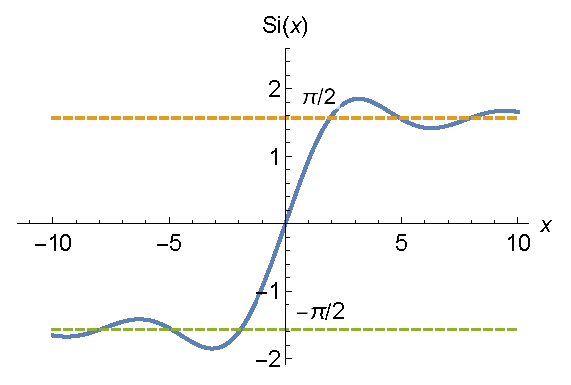
\includegraphics[width=0.3\textwidth]{si.eps}
%     \caption{\footnotesize 正弦积分}
% \end{wrapfigure}
    \begin{equation*}
        \begin{array}{ll}
            \displaystyle{\trm{sinc}(x) = \frac{\sin(x)}{x}} &
            \displaystyle{\trm{Si}(x) = \int_{0}^{x} \trm{sinc}(t) \trm{d}t}  \\
            \displaystyle{\trm{cosc}(x) = \frac{\cos(x)}{x}} &
            \displaystyle{\trm{Ci}(x) = \int_{0}^{x} \trm{cosc}(t) \trm{d}t}  \\
            \displaystyle{\trm{sinhc}(x) = \frac{\sinh(x)}{x}} &
            \displaystyle{\trm{Shi}(x) = \int_{0}^{x} \trm{sinhc}(t) \trm{d}t}  \\
            \displaystyle{\trm{coshc}(x) = \frac{\cos(x)}{x}} &
            \displaystyle{\trm{Chi}(x) = \int_{0}^{x} \trm{coshc}(t) \trm{d}t}  \\
        \end{array}
    \end{equation*}
% \begin{figure}[H]
%    \centering
%    \subfigure[]{
%        \label{fig:a} %% label for first subfigure
%        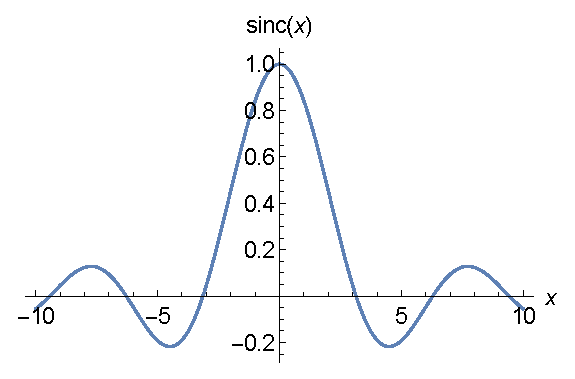
\includegraphics[width=0.32\textwidth]{sinc.eps}
%    }
%    \subfigure[]{
%        \label{fig:b} %% label for secondsubfigure
%        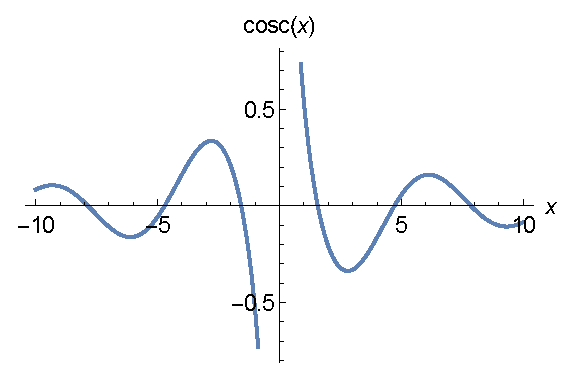
\includegraphics[width=0.32\textwidth]{cosc.eps}
%    }
% \end{figure}
% \begin{figure}[H]
%     \centering
%    \subfigure[]{
%        \label{fig:c} %% label for secondsubfigure
%        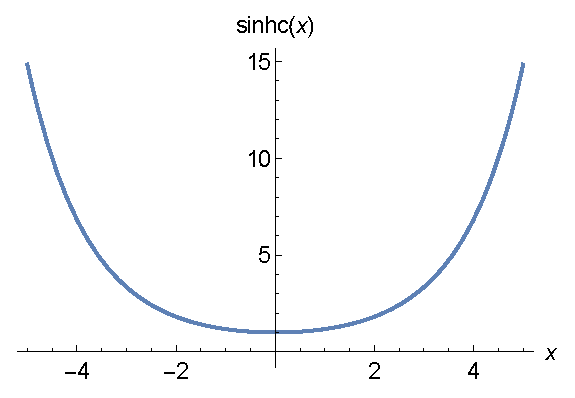
\includegraphics[width=0.32\textwidth]{sinhc.eps}
%    }
%    \subfigure[]{
%        \label{fig:d} %% label for secondsubfigure
%        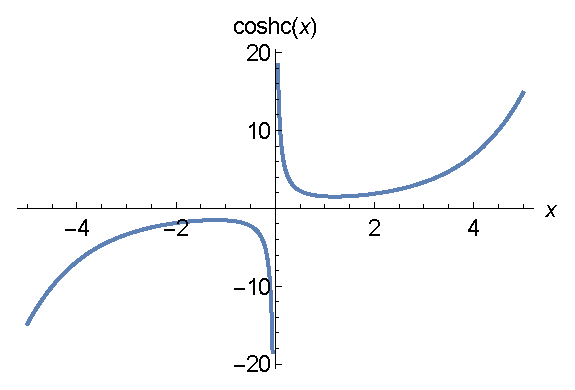
\includegraphics[width=0.32\textwidth]{coshc.eps}
%    }
%    \caption{composited function}
%    \label{figb} %% label for entire figure
% \end{figure}
    \item[(3)] 指数积分(exponentiation integral)
    \[ \trm{Ei}(x) = \int_{0}^{x} \frac{e^{-t}}{t} \trm{d}t \]
    \item[(4)] 对数积分(logarithm integral)
    \[ \trm{li}(x) = \int_{0}^{x} \frac{\ln(t)}{t} \trm{d}t \]
\end{itemize}

\section{柱函数(贝塞尔函数)系}

\subsection{为什么会有这个函数?}

贝塞尔函数是贝塞尔方程的解,贝塞尔方程指的是
\[x^2y″ + xy′ + (x^2-\alpha^2)y = 0\]
这个方程常常伴随着柱坐标系出现,以下列举两种情况.

\begin{itemize}
    \item[(1)] 拉普拉斯方程为\(\nabla^2 u =0\),根据柱坐标系与直角坐标系的关系:
    \[\rho = \sqrt{x^2+y^2} \qquad \theta = \arg(x+iy) \qquad z = z\]
    在三维柱坐标系下展开得到
    \[\frac{1}{\rho}\frac{\partial}{\partial \rho}\left(\rho\frac{\partial u}{\partial \rho}\right) + \frac{1}{\rho^2}\frac{\partial^2 u}{\partial \theta^2} + \frac{\partial^2 u}{\partial z^2} = 0\]
    分离变量,令\(u(\rho,\theta,z)=f(\rho)g(\theta)h(z)\),回代并在等号两边同时乘以\(\displaystyle{\frac{r^2}{f(\rho)g(\theta)h(z)}}\),得到
    \[\frac{\rho}{f(\rho)}\frac{\partial}{\partial \rho}\left(\rho f'(\rho)\right) + \frac{g''(\theta)}{g(\theta)} + \rho^2\frac{h''(z)}{h(z)} = 0\]
    左边是三个单项式相加的形式,其中参数\(\theta\)只与第二个单项式\(\displaystyle{\frac{g''(\theta)}{g(\theta)}}\)有关,然而右边为常数\(0\),这说明\(\displaystyle{\frac{g''(\theta)}{g(\theta)}}\)必须是一个常数,否则当\(\theta\)发生变化后,左边的值就会发生变化,而这种变化是与\(\theta\)无关的参数\(\rho,z\)所无法抵消的. 所以设\(\displaystyle{\frac{g''(\theta)}{g(\theta)}} = -n^2\),回代的同时两边同除\(r^2\),得到
    \[\frac{1}{\rho f(\rho)}\frac{\partial}{\partial \rho}\left(\rho f'(\rho)\right) -\frac{n^2}{r^2} + \frac{h''(z)}{h(z)} = 0\]
    对\(\displaystyle{\frac{h''(z)}{h(z)}}\)使用相同的手法,令其为\(k_z^2\),回代的同时两边再同乘\(f(\rho)\),得到
    \[\frac{1}{\rho}\frac{\partial}{\partial \rho}\left(\rho f'(\rho)\right) + \left(k_z^2-\frac{n^2}{\rho^2}\right)f(\rho) = 0\]
    两边同乘\(r^2\)整理得到
    \[\rho^2f''(\rho)+rf'(\rho)+[(k_z\rho)^2-n^2]f(\rho) = 0\]
    这就得到了贝塞尔方程.
    \item[(2)] 热传导方程为\(\displaystyle{\frac{\partial u}{\partial t} = a^2\nabla^2 u}\),在二维
\end{itemize}

\begin{definition}{贝塞尔函数}
    第一类贝塞尔函数
    \[J_{\alpha}(x) = \sum_{n=0}^{\infty} \frac{(-1)^{n}}{n!\Gamma (n+\alpha +1)}{\left({\frac {x}{2}}\right)}^{2n+\alpha}\]
    第二类贝塞尔函数
    \[Y_{\alpha}(x) = \frac{J_{\alpha}(x)\cos(\alpha\pi)-J_{-\alpha}(x)}{\sin(\alpha\pi)}\]
    汉克尔函数
    \[
        \begin{aligned}
            H_{\alpha }^{(1)}(x) &= J_{\alpha }(x)+iY_{\alpha }(x) \\ 
            H_{\alpha}^{(2)}(x) &= J_{\alpha}(x)-iY_{\alpha}(x) 
        \end{aligned}
    \]
    修正贝塞尔函数
    \[
        \begin{aligned}
            I_{\alpha }(x) &= i^{-\alpha }J_{\alpha }(ix) \\
            K_{\alpha }(x) &= \frac {\pi }{2}{\frac {I_{-\alpha }(x)-I_{\alpha }(x)}{\sin \alpha \pi }} 
        \end{aligned}
    \]
    球贝塞尔函数
    \[
        \begin{aligned}
            j_{n}(x) &= \sqrt{\frac {\pi }{2x}}J_{n+{\frac {1}{2}}}(x) \\
            y_{n}(x) &= \sqrt{\frac {\pi }{2x}}Y_{n+{\frac {1}{2}}}(x)
        \end{aligned}
    \]
    球汉克尔函数
    \[
        \begin{aligned}
            h_{n}^{(1)}(x) &= j_{n}(x)+iy_{n}(x) \\
            h_{n}^{(2)}(x) &= j_{n}(x)-iy_{n}(x)
        \end{aligned}
    \]
\end{definition}

\begin{proposition}{某个算不出来的积分}
    利用修正贝塞尔函数可以得到
    \[\int e^{\cos(x)}\trm{d}x = \int e^{\sin(x)}\trm{d}x = \int e^{\cos(x)}\trm{d}t=I_0(1)x+2\sum_{n=1}^{\infty}I_n(1)\frac{\sin(nx)}{n} + C\]
\end{proposition}

\textit{
    令\(u=x-\dfrac{\pi}{2}\),则根据第二类换元法
    \[\int e^{\sin(x)}\trm{d}x = \int e^{\sin(u+\pi/2)}\trm{d}\left(u+\frac{\pi}{2}\right)=\int e^{\cos(u)}\trm{d}u\]
    接着对\(e^{\cos(x)}\)作三角函数项的傅里叶展开
    \[e^{\cos(x)}=\frac{1}{2}a_0+\sum_{n=1}^{\infty}\left(a_n\cos(nx)+b_n\sin(nx)\right)\]
    代入修正贝塞尔函数\(\displaystyle{I_n(z)=\frac{1}{\pi}\int_{0}^{\pi}e^{z\cos(x)}\cos(nx)\trm{d}x}\)
    \[
        \begin{aligned}
            a_n&=\frac{1}{\pi}\int_{-\pi}^{\pi}e^{\cos(x)}\cos(nx)\trm{d}x=2I_n(1) \\
            b_n&=\frac{1}{\pi}\int_{-\pi}^{\pi}e^{\cos(x)}\sin(nx)\trm{d}x=0
        \end{aligned}
    \]
    于是
    \[e^{\cos(x)}=I_0(1)+2\sum_{n=1}^{\infty}I_n(1)\cos(nx)\]
    逐项积分就是
    \[\int e^{\cos(x)}\trm{d}t=I_0(1)x+2\sum_{n=1}^{\infty}\frac{I_n(1)}{n}\sin(nx) + C\]
}

\section{勒让德多项式(球多项式)}

\subsection{利用正交性导出}

泰勒展开告诉我们,\(\{x^n\}_{n=0}^{\infty}\)是\(C(\mathbb{R})\)的一个完备基底,但是这个基底却不是正交的,甚至在任意一个子集上都不正交,理由很简单,求内积时\(\langle x^n, x^n \rangle\)和\(\langle x^{n-1}, x^{n+1} \rangle\)的被积函数是相同的,而如果正交的话前者应为非零,后者应为零,矛盾. 于是我们自然就会思考将它们正交化,做出一组完备的正交基底.
\begin{reference}
    回顾线性代数的知识,当向量\(\{\vec{\alpha}_k\}_{k=1}^{n}\)线性无关时,它们可以张成\(n\)维线性空间,而该线性空间的一组完备正交基底\(\{\vec{\beta}_k\}_{k=1}^{n}\)可以根据\(\{\vec{\alpha}_k\}_{k=1}^{n}\)利用格拉姆-施密特正交化构造出来:
    \[
        \vec{\beta}_k = 
        \left\{
            \begin{aligned}
                & \vec{\alpha}_k & k=1 \\
                & \vec{\alpha}_k - \sum_{m=0}^{k-1}\frac{\langle \vec{\alpha}_k, \vec{\beta}_m \rangle}{\langle \vec{\beta}_m, \vec{\beta}_m \rangle}\vec{\beta}_{m} & k > 1
            \end{aligned}
        \right.
    \]
\end{reference}

接下来要做的事是选取一个好的函数空间,\(C(\mathbb{R})\)并不是一个好的选择,因为\(\lambda x.1\)在\(\mathbb(R)\)上的积分是无穷. 所以我们选择了\(C([-1,1])\). 遵循格拉姆-施密特正交化方法,在区间\([-1,1]\)上,有:
\begin{align*}
    p_0(x) &= 1 \\
    p_1(x) &= x-\frac{\langle x, 1 \rangle}{\langle 1,1 \rangle} \\
    &= x - \frac{\int_{-1}^{1} x \trm{d}x}{\int_{-1}^{1} 1\trm{d}x} = x \\
    p_2(x) &= x^2 - \frac{\langle x^2, 1 \rangle}{\langle 1,1 \rangle} - \frac{\langle x^2, x \rangle}{\langle x,x \rangle}x \\
    &= x^2 - \frac{\int_{-1}^{1} x^2 \trm{d}x}{\int_{-1}^{1} 1\trm{d}x} - \frac{\int_{-1}^{1} x^3 \trm{d}x}{\int_{-1}^{1} x^2 \trm{d}x}x = x^2-\frac{1}{3} \\
    p_3(x) &= x^3 - \frac{\langle x^3, 1 \rangle}{\langle 1,1 \rangle} - \frac{\langle x^3, x \rangle}{\langle x,x \rangle}x - \frac{\langle x^3, x^2-\frac{1}{3} \rangle}{\langle x^2-\frac{1}{3},x^2-\frac{1}{3} \rangle}(x^2-\frac{1}{3}) \\
    &= x^3 - \frac{\int_{-1}^{1} x^3 \trm{d}x}{\int_{-1}^{1} 1\trm{d}x} - \frac{\int_{-1}^{1} x^4 \trm{d}x}{\int_{-1}^{1} x^2 \trm{d}x}x - \frac{\int_{-1}^{1} x^3(x^2-\frac{1}{3}) \trm{d}x}{\int_{-1}^{1} (x^2-\frac{1}{3})^2 \trm{d}x}(x^2-\frac{1}{3}) = x^3 - \frac{3}{5}x
\end{align*}

我们希望得到的正交基底的性质尽可能模仿\(\{x^n\}_{n=0}^{\infty}\)的性质,后者简单列举两条
\begin{itemize}
    \item [\(\bullet\)] \((\lambda x.x^n)(1) = 1\)
    \item [\(\bullet\)] 在区间\([-1,1]\)上,\(\langle x^n,x^n \rangle = \dfrac{2}{2n+1}\)
\end{itemize}

\section{椭圆函数系}

\section{超几何函数系}

超几何函数最初由高斯定义,在勒奇超越函数的基础上更推进一步. 最终得到的推广的超几何函数是一个包容性非常强的函数,以上提到的大部分特殊函数,包括勒奇超越函数系、贝塞尔函数系和椭圆函数系都是它的特殊情况,因此超几何函数可以非常深刻地揭示以上众多特殊函数的共性.

\begin{definition}{超几何函数}
    上升阶乘(rising factorial)或伯赫哈默尔符号(Pochhammer symbol):
    \[n^{(m)} = \left\{\begin{aligned} &1 & m=0 \\ & \prod_{k=m}^{n+m-1}k = n(n+1)\cdots(n+m-1) & m > 0 \end{aligned}\right.\]
    合流超几何函数(confluent hypergeometric function)或库莫函数(Kummer function)
    \[M(a,b,z) = \sum_{n=0}^{\infty}\frac{a^{(n)}}{b^{(n)}}\frac{z^n}{n!}\]
    超几何函数(hypergeometric function)
    \[_2F_1(a,b;c;z) = \sum_{n=0}^{\infty}\frac{a^{(n)}b^{(n)}}{c^{(n)}}\frac{z^n}{n!}\]
    推广的超几何函数(generalized hypergeometric function)
    \[_pF_q(a_1, a_2, \cdots, a_p; b_1, b_2, \cdots, b_q;z) = \sum_{n=0}^{\infty}\frac{a_1^{(n)}a_2^{(n)}\cdots a_p^{(n)}}{b_1^{(n)}b_2^{(n)}\cdots b_q^{(n)}}\frac{z^n}{n!}\]
\end{definition}

\end{document}

